%%%%%%%%%%%%%%%%%%%%%%%%%%%%%%%%%%%%%%%%%
% The Legrand Orange Book
% LaTeX Template
% Version 3.1 (February 18, 2022)
%
% This template originates from:
% https://www.LaTeXTemplates.com
%
% Authors:
% Vel (vel@latextemplates.com)
% Mathias Legrand (legrand.mathias@gmail.com)
%
% License:
% CC BY-NC-SA 4.0 (https://creativecommons.org/licenses/by-nc-sa/4.0/)
%
% Compiling this template:
% This template uses biber for its bibliography and makeindex for its index.
% When you first open the template, compile it from the command line with the 
% commands below to make sure your LaTeX distribution is configured correctly:
%
% 1) pdflatex main
% 2) makeindex main.idx -s indexstyle.ist
% 3) biber main
% 4) pdflatex main x 2
%
% After this, when you wish to update the bibliography/index use the appropriate
% command above and make sure to compile with pdflatex several times 
% afterwards to propagate your changes to the document.
%
%%%%%%%%%%%%%%%%%%%%%%%%%%%%%%%%%%%%%%%%%

%----------------------------------------------------------------------------------------
%	PACKAGES AND OTHER DOCUMENT CONFIGURATIONS
%----------------------------------------------------------------------------------------

\documentclass[
	12pt, % Default font size, select one of 10pt, 11pt or 12pt
	fleqn, % Left align equations
	a4paper, % Paper size, use either 'a4paper' for A4 size or 'letterpaper' for US letter size
	%oneside, % Uncomment for oneside mode, this doesn't start new chapters and parts on odd pages (adding an empty page if required), this mode is more suitable if the book is to be read on a screen instead of printed
]{LegrandOrangeBook}

% Book information for PDF metadata, remove/comment this block if not required 
\hypersetup{
	pdftitle={Title}, % Title field
	pdfauthor={Author}, % Author field
	pdfsubject={Subject}, % Subject field
	pdfkeywords={Keyword1, Keyword2, ...}, % Keywords
	pdfcreator={LaTeX}, % Content creator field
}

\usepackage{algorithm}
\usepackage{algpseudocode}
\usepackage{wrapfig}
\usepackage{hyperref}
\addbibresource{sample.bib} % Bibliography file

\definecolor{ocre}{RGB}{243, 102, 25} % Define the color used for highlighting throughout the book

\chapterimage{orange1.jpg} % Chapter heading image
\chapterspaceabove{6.5cm} % Default whitespace from the top of the page to the chapter title on chapter pages
\chapterspacebelow{6.75cm} % Default amount of vertical whitespace from the top margin to the start of the text on chapter pages

%----------------------------------------------------------------------------------------

\begin{document}

%----------------------------------------------------------------------------------------
%	TITLE PAGE
%----------------------------------------------------------------------------------------

\titlepage % Output the title page
	{
\includegraphics[width=\paperwidth]{background.pdf}} % Code to output the background image, which should be the same dimensions as the paper to fill the page entirely; leave empty for no background image
	{ % Title(s) and author(s)
		\centering\sffamily % Font styling
		{\Huge\bfseries Math for Computer Science\par} % Book title
		\vspace{16pt} % Vertical whitespace
		{\LARGE Bridging Theory and Practice} % Subtitle
		\vspace{24pt} % Vertical whitespace
		{\huge\bfseries \\ Eric Yang Xingyu\par} % Author name
	}

%----------------------------------------------------------------------------------------
%	COPYRIGHT PAGE
%----------------------------------------------------------------------------------------

\thispagestyle{empty} % Suppress headers and footers on this page

~\vfill % Push the text down to the bottom of the page

\noindent Copyright \copyright\ 2024 Eric Yang Xingyu\\ % Copyright notice

\noindent \textsc{Published by Publisher}\\ % Publisher
This \LaTeX \space template is from 
\noindent \textsc{\href{https://www.latextemplates.com/template/legrand-orange-book}{book-website.com}}\\ % URL

\noindent Licensed under the Creative Commons Attribution-NonCommercial 4.0 License (the ``License''). You may not use this file except in compliance with the License. You may obtain a copy of the License at \url{https://creativecommons.org/licenses/by-nc-sa/4.0}. Unless required by applicable law or agreed to in writing, software distributed under the License is distributed on an \textsc{``as is'' basis, without warranties or conditions of any kind}, either express or implied. See the License for the specific language governing permissions and limitations under the License.\\ % License information, replace this with your own license (if any)

\noindent \textit{First amendment, March 2024} % Printing/edition date

%----------------------------------------------------------------------------------------
%	TABLE OF CONTENTS
%----------------------------------------------------------------------------------------

\pagestyle{empty} % Disable headers and footers for the following pages

\tableofcontents % Output the table of contents

\listoffigures % Output the list of figures, comment or remove this command if not required

\listoftables % Output the list of tables, comment or remove this command if not required

\pagestyle{fancy} % Enable default headers and footers again

\cleardoublepage % Start the following content on a new page

%----------------------------------------------------------------------------------------
%	PART
%----------------------------------------------------------------------------------------

\part{Introductory Topics}

%----------------------------------------------------------------------------------------
%----------------------------------------------------------------------------------------

\chapterimage{chap1.png} % Chapter heading image
\chapterspaceabove{4.25cm} % Whitespace from the top of the page to the chapter title on chapter pages
\chapterspacebelow{7.25cm} % Amount of vertical whitespace from the top margin to the start of the text on chapter pages

%------------------------------------------------

\chapter{Mathematical Proof Strategy}
The first Chapter of this book focus only on the most essential part of mathematics, proofs. Proofs are the very essence of mathematics, 
serving as the definitive tool for establishing the truth within this discipline of absolute certainty. Unlike empirical sciences, where conclusions are 
drawn based on observation and experimentation subject to uncertainties, mathematical proofs provide incontrovertible evidence that a statement is true. 
They are the architects of mathematical theory, constructing a framework of knowledge that is both logical and immutable. Through proofs, we not 
only validate conjectures but also weave a tapestry of interconnected truths, each supported by the unshakable foundation of previously proven results. 
This interconnectedness ensures that mathematical knowledge, once proven, becomes a permanent addition to the collective human understanding, transcending time 
and offering a universal language spoken by all cultures in the language of logic and reason.

%------------------------------------------------
\section{Propositions}
The angles in a triangle add up to 180 degrees; the sum of any two even numbers is even. Statement as such is so common in mathematics, which we call proposition.
	\begin{definition}[Proposition]
		A proposition is a declarative sentence that is either true or false. 
		Propositions are the fundamental building blocks of mathematical reasoning, as they can be clearly judged to be true or false.
	\end{definition}
	Propositions have the following characteristics:
	\begin{enumerate}
		\item \textbf{Definiteness:} Propositions must be clear and unambiguous so that they can be definitively judged to be true or false.
		\item \textbf{Exclusivity:} Propositions admit no middle ground between true and false.
		\item \textbf{Objectivity:} Propositions represent objective facts, not subjective opinions or questions.
	\end{enumerate}

\noindent	Propositions are essential and crucial for proof, this is because
	\begin{itemize}
		\item \textbf{Foundation:} Propositions are the foundation upon which logical reasoning is built.
		\item \textbf{Validity:} Proving the validity of a proposition reinforces the truthfulness of a statement.
		\item \textbf{Interconnectedness:} Propositions are interconnected; proving one can help establish the truth of others.
	\end{itemize}

	In mathematical discourse, the clarity and truth of propositions are paramount. Understanding the nature of propositions (truth, falsity, and reasoning) is essential for constructing and understanding mathematical arguments.	
Commonly, Propositions are categorized by the \textbf{truth value}, which we will discuss
in Boolean Algebra, and we call a proposition true proposition when the statement is factually correct, while false
proposition, vice versa. Most importantly: \textbf{If a proposition is true, it can be proven}.
\section*{Converse, Inverse, and Contrapositive}
In the study of logic, particularly within the context of mathematical reasoning, we come across several important concepts that relate to conditional statements. A conditional statement is typically of the form "If \(P\), then \(Q\)", denoted \(P \rightarrow Q\). Here we define and discuss the converse, inverse, and contrapositive of a conditional statement.

\subsection*{Converse}
The converse of a statement flips the hypothesis and the conclusion. For the statement \(P \rightarrow Q\), the converse is \(Q \rightarrow P\). It is important to note that the truth of a converse is not necessarily the same as the truth of the original statement.

\subsection*{Inverse}
The inverse of a statement negates both the hypothesis and the conclusion. For the statement \(P \rightarrow Q\), the inverse is \(\neg P \rightarrow \neg Q\), where \(\neg\) denotes negation. Similar to the converse, the truth of the inverse is not dependent on the truth of the original statement.

\subsection*{Contrapositive}
The contrapositive of a statement negates and flips the hypothesis and the conclusion. For the statement \(P \rightarrow Q\), the contrapositive is \(\neg Q \rightarrow \neg P\). Unlike the converse and the inverse, the truth of the contrapositive is always the same as the truth of the original statement. This property is often used in mathematical proofs, particularly in \textbf{proofs by contradiction}, which we will discuss in successive sections.

\section{Direct Proof}
	\subsection*{Framework of Direct Proof}
	A direct proof is a fundamental method in mathematics used to establish the truth of a
	given statement, typically a theorem or proposition. It is characterized by a straightforward
	and logical progression from known facts or axioms to the conclusion. The approach
	of a direct proof is to assume that the premises (initial assumptions or known truths)
	are correct and then to use logical reasoning and established mathematical principles to
	demonstrate that the conclusion necessarily follows from these premises. Here's a general
	structure of how a direct proof works:
	\begin{enumerate}
		\item Start with Known Facts or Assumptions: Begin with what is already known or
		assumed to be true. These can be definitions, previously proven theorems, or given
		premises.
		\item Logical Argumentation: Use logical reasoning and mathematical operations to derive
		new information from these known facts. This process often involves applying
		definitions, using the properties of mathematical operations, and invoking previously
		established theorems.
		\item Arrive at the Conclusion: The final step is to show that the statement you set out
		to prove is a logical consequence of the initial assumptions. The conclusion should
		follow naturally and unavoidably from the previous steps.
	\end{enumerate}
	To illustrate:
    \begin{example}
	
		Prove that if \( n \) is an odd integer, then \( n^2 \) is also odd.
	
    \end{example}

    \begin{proof}
		Assume \( n \) is an odd integer. By definition, an odd integer can be written as \( n = 2k + 1 \) where \( k \) is an integer.
		
		Squaring both sides of this equation, we get
		\[ n^2 = (2k + 1)^2 = 4k^2 + 4k + 1 = 2(2k^2 + 2k) + 1. \]
		
		Let \( m = 2k^2 + 2k \), which is an integer since it is a sum of integers. Therefore, we can express \( n^2 \) as
		\[ n^2 = 2m + 1. \]
		
		This is the form of an odd integer. Thus, we have shown that if \( n \) is an odd integer, then \( n^2 \) is also odd.
		\end{proof}
  
		We can see that the idea of direct proof is something everyone can understand, however,
		what is really challenging is to find the specific know facts to assist the proof. Here
		are more exercises on direct proof for reference.
        
		\subsection{Exercises}
		\begin{exercise}
			Prove that if \( n \) is an even integer, then \( n^2 \) is also even.
		\end{exercise}
		Hint: follow the procedure of the example of odd number, using the definition of even integer.
		\begin{proof}
        Assume \( n \) is an even integer. By definition, an even number can be expressed as \( n = 2k \) where \( k \) is an integer.
        
        Squaring both sides of this equation, we get:
        \[ n^2 = (2k)^2 = 4k^2 = 2(2k^2). \]
        
        Since \( 2k^2 \) is an integer (let's call it \( m \)), we can express \( n^2 \) as \( 2m \), which is the definition of an even number.
        
        Hence, if \( n \) is an even integer, then \( n^2 \) is also even.
        \end{proof}
        \begin{exercise}
			Prove that the sum of two even integers is even.
		\end{exercise}
		Hint: Use the definition of an even integer.
        \begin{proof}
        Let \( a \) and \( b \) be even integers. By the definition of even integers, there exist integers \( k \) and \( m \) such that \( a = 2k \) and \( b = 2m \).
        
        The sum of \( a \) and \( b \) is:
        \[ a + b = 2k + 2m = 2(k + m). \]
        
        Let \( n = k + m \), which is an integer since both \( k \) and \( m \) are integers. Hence, \( a + b = 2n \).
        
        Since \( a + b \) is two times an integer, it is even by definition. This concludes the proof.
        \end{proof}
		
		\begin{exercise}\label{ex1.3}
			Prove that for any positive integer \( n \), \( n^3 + 2n \) is divisible by 3.
		\end{exercise}
			Hint: Factorize \( n^3 + 2n \) and use the properties of divisibility.
        \begin{proof}
         Consider the expression \( n^3 + 2n \). This can be factored as:
        \[ n^3 + 2n = n(n^2 + 2) = n(n^2 - 1 + 3) = n(n+1)(n-1)+3n. \]
        
        Notice that \( n^2 + 2 \) can be written as \( (n^2 - 1) + 3 = (n+1)(n-1) + 3 \). The terms \( n + 1 \), $n$, and \( n - 1 \) are three consecutive integers, so one of them must be multiple of 3. Therefore, $n(n+1)(n-1)$ can be denoted by $3m$, where $m$ is a positive integer, and the expression is equivalent to $3(m+n)$. 
        
        Hence, for any positive integer \( n \), \( n^3 + 2n \) is divisible by 3.
        
        \end{proof}
    \begin{remark}
        Considering there are still concepts that we haven't covered in Boolean algebra and number theory, the exercises in this chapter will be more basic than other chapters. What's really important in this chapter is not to finish difficult proof, but grasp the idea of proving.
    \end{remark}

\section{Proof by Cases}
    Sometimes, to draw a specific conclusion, we must make multiple or even infinite assumptions (The latter we will discuss in \textbf{Strong Mathematical induction}). This proof pattern stands alone from direct proof, as when we use this method, the proof itself could still be direct or indirect.
    \subsection*{Framework of Proof by Cases}
        \begin{proof}
        The proof is by cases. We consider each possible case and show that the theorem holds in each case.
        
        \textbf{Case 1:} [Description of Case 1]
        \begin{proof}[Proof of Case 1]
        Present the proof for Case 1 here. Use logical reasoning and mathematical principles to demonstrate that the theorem holds under the assumptions of Case 1.
        \end{proof}
        
        \textbf{Case 2:} [Description of Case 2]
        \begin{proof}[Proof of Case 2]
        Similarly, present the proof for Case 2 here, showing that the theorem is valid in this scenario as well.
        \end{proof}

% Add more cases as necessary

\textit{Final Conclusion:} Since the theorem holds in all possible cases, we conclude that the theorem is proved.
\end{proof}

    Here is an example of proof by cases.
    \begin{example}
        
            Prove that the sum of any three consecutive integers is divisible by 3.
            
    \end{example}

    \begin{proof}
            Let the three consecutive integers be \( n \), \( n+1 \), and \( n+2 \), where \( n \) is an integer. We consider three cases for \( n \), based on the division by 3.
            
            \textbf{Case 1:} \( n \) is of the form \( 3k \) for some integer \( k \).
            
            \textbf{Case 2:} \( n \) is of the form \( 3k + 1 \) for some integer \( k \).
            
            \textbf{Case 3:} \( n \) is of the form \( 3k + 2 \) for some integer \( k \).
            
            In each case, the sum of \( n \), \( n+1 \), and \( n+2 \) can be expressed as:
            
            For Case 1: \( (3k) + (3k + 1) + (3k + 2) = 9k + 3 = 3(3k + 1) \), it is divisible by 3.
            
            For Case 2: \( (3k + 1) + (3k + 2) + (3k + 3) = 9k + 6 = 3(3k + 2) \), it is divisible by 3.
            
            For Case 3: \( (3k + 2) + (3k + 3) + (3k + 4) = 9k + 9 = 3(3k + 3) \), it is divisible by 3.
            
            In each of the three cases, the sum is a multiple of 3. Therefore, we conclude that the sum of any three consecutive integers is divisible by 3.
            \end{proof}
            
\begin{remark}
    As mentioned in direct proof, the idea of proving is always simple and easy to understand. For proof by cases, the toughest part is also finding all the cases needed to prove a certain conclusion.
\end{remark}
\subsection{Exercises}
\begin{exercise}
			Prove that the product of two consecutive integers is always even.
\end{exercise}
		Hint: Express the consecutive integers as \( n \) and \( n + 1 \).
\begin{proof}
Consider two consecutive integers, \( n \) and \( n + 1 \), where \( n \) is an integer. The product of these two integers is \( n(n + 1) \).

We have two cases to consider:

\textbf{Case 1:} If \( n \) is even, then it can be written as \( n = 2k \) for some integer \( k \). The product is then \( n(n + 1) = 2k(2k + 1) \), which is even because it is divisible by 2.

\textbf{Case 2:} If \( n \) is odd, then \( n + 1 \) is even. In this case, \( n + 1 = 2k \) for some integer \( k \). The product is then \( n(n + 1) = n(2k) \), which is even because it is divisible by 2.

In either case, the product of \( n \) and \( n + 1 \) is even. Therefore, the product of two consecutive integers is always even.
\end{proof}
\begin{exercise}
	Prove that if \( n \) is an integer, then \( n(n+1) \) is even.
\end{exercise}
Hint: Consider the cases where n is even and where n is odd separately.
\begin{proof}
We will consider two cases based on the parity of \( n \).

\textbf{Case 1:} \( n \) is even.

Let \( n = 2k \) for some integer \( k \). Then \( n(n+1) = 2k(2k+1) \). Since \( 2k \) is even, the product \( 2k(2k+1) \) is also even because the product of an even number and any other integer is even.

\textbf{Case 2:} \( n \) is odd.

Let \( n = 2k+1 \) for some integer \( k \). Then \( n(n+1) = (2k+1)(2k+2) \). Here \( (2k+2) \) is even, and thus the product \( (2k+1)(2k+2) \) is even because the product of an even number and any other integer is even.

In both cases, whether \( n \) is even or odd, \( n(n+1) \) is even. Hence, we have shown that for any integer \( n \), the product \( n(n+1) \) is always even.
\end{proof}

\begin{exercise}
Prove that for any integer \( n \), \( n^2 + 4 \) cannot be a prime number if \( n > 1 \).
\end{exercise}
Hint: Consider the cases where n is even and where n is odd.
\begin{proof}
Consider two cases based on the parity of \( n \).

\textbf{Case 1:} \( n \) is even.

Let \( n = 2k \) for some integer \( k \). Then \( n^2 + 4 \) becomes \( (2k)^2 + 4 = 4k^2 + 4 = 4(k^2 + 1) \). Since \( k^2 + 1 \) is an integer greater than 1, \( 4(k^2 + 1) \) is not prime because it has factors other than 1 and itself, namely 4 and \( k^2 + 1 \).

\textbf{Case 2:} \( n \) is odd.

Let \( n = 2k + 1 \) for some integer \( k \). Then \( n^2 + 4 \) becomes \( (2k + 1)^2 + 4 = 4k^2 + 4k + 1 + 4 = 4k^2 + 4k + 5 \). This can be factored as \( (2k + 1)(2k + 3) \), which are two consecutive odd numbers. Since both \( 2k + 1 \) and \( 2k + 3 \) are factors greater than 1 but not the expression itself, the product is not prime.
Therefore, in both cases, whether \( n \) is even or odd, \( n^2 + 4 \) is not a prime number.
\end{proof}

\begin{exercise}

Prove that for any integer \( n \), the expression \( n^5 - n \) is divisible by 30.

\end{exercise}
Hint: Consider divisibility of 5 and 6 (2 and 3), and prove by cases accordingly. 
\begin{proof}
To prove that \( n^5 - n \) is divisible by 6, it suffices to show that it is divisible by 2, 3, and 5.

First, observe that \( n^5 - n = n(n^4 - 1) \).

\textbf{Divisibility by 2:} 
\begin{itemize}
  \item If \( n \) is even, then \( n^5 - n \) is clearly even since it is a multiple of \( n \).
  \item If \( n \) is odd, \( n^4 - 1 \) is even because \( n^4 \) is odd and \( n^4 - 1 \) is one less than an odd number, making it even.
\end{itemize}

\textbf{Divisibility by 3:} \\ 
Any integer \( n \) is either a multiple of 3, one more than a multiple of 3, or two more than a multiple of 3. That is, \( n \) can be written as \( 3k \), \( 3k + 1 \), or \( 3k + 2 \) for some integer \( k \).

\begin{itemize}
    \item If \( n = 3k \), then \( n^5 - n = (3k)^5 - 3k \) is clearly a multiple of 3.
    \item If \( n = 3k + 1 \), then \( n^5 - n = (3k + 1)^5 - (3k + 1) \). Expanding \( (3k + 1)^5 \) using the binomial theorem, all terms except the last are multiples of 3, and the last term \( 1^5 \) minus \( 3k + 1 \) leaves \( -3k \), which is a multiple of 3.
    \item If \( n = 3k + 2 \), a similar expansion shows that \( n^5 - n \) is a multiple of 3.
\end{itemize}

Thus, \( n^5 - n \) is divisible by 3.

\textbf{Divisibility by 5:} 
For any integer \( n \), we can express \( n \) in one of the following forms, where \( k \) is an integer:
\begin{enumerate}
    \item \( n = 5k \) (where \( n \) is a multiple of 5)
    \item \( n = 5k + 1 \)
    \item \( n = 5k + 2 \)
    \item \( n = 5k + 3 \)
    \item \( n = 5k + 4 \)
\end{enumerate}

We will prove that \( n^5 - n \) is divisible by 5 for each case. Since we are working modulo 5, we only need to consider the last digit of \( n \) when raised to the fifth power due to the cyclicity of powers modulo 5.

\begin{itemize}
    \item For \( n = 5k \): \( n^5 - n = (5k)^5 - 5k \). Clearly, both terms are divisible by 5.
    \item For \( n = 5k + 1 \): \( n^5 - n = (5k + 1)^5 - (5k + 1) \). When expanded, each term of \( (5k + 1)^5 \) except the last will contain a factor of \( 5k \) and thus be divisible by 5. The last term \( 1^5 = 1 \), and subtracting \( 5k + 1 \) leaves a result which is still divisible by 5.
    \item For \( n = 5k + 2 \): \( n^5 - n = (5k + 2)^5 - (5k + 2) \). Again, each term in the expansion of \( (5k + 2)^5 \), except the last, will be divisible by 5. The last term will be \( 2^5 = 32 \), which is congruent to 2 modulo 5, and subtracting \( (5k + 2) \) leaves a result divisible by 5.
    \item For \( n = 5k + 3 \) and \( n = 5k + 4 \), a similar argument holds as for \( n = 5k + 1 \) and \( n = 5k + 2 \), respectively.
\end{itemize}

In all cases, \( n^5 - n \) is divisible by 5. This completes the proof for Case 3.

Therefore, \( n^5 - n \) is divisible by 2, 3, and 5, and hence by 30.
\end{proof}


%----------------------------------------------------------------------

\section{Indirect Proof}
    An indirect proof is a powerful method in mathematics used to prove a statement by showing that the negation leads to a contradiction or by proving the contrapositive of the statement. We will discuss proof by contradiction and proof by contrapositive separately.

\subsection{Proof by Contradiction}

Proof by contradiction is a critical reasoning technique used extensively in mathematics and logic. Its importance lies in its ability to confirm the truth of a statement by demonstrating that assuming the opposite leads to an illogical or impossible conclusion. This method is particularly valuable because it can sometimes prove assertions that are otherwise difficult to demonstrate directly. It is a cornerstone of mathematical reasoning and is often used to establish fundamental theorems that form the bedrock of mathematical theories. The use of this technique highlights the rigorous nature of mathematical proof and emphasizes the importance of logical consistency within mathematical frameworks.

Here is an abstract template for proof by contradiction:

Suppose, for the sake of contradiction, that the statement we wish to prove is false.

\begin{enumerate}
    \item State the negation of the theorem or proposition you are trying to prove.
    \item Use logical reasoning and established mathematical principles to derive consequences of this assumption.
    \item Show that these consequences lead to a contradiction, something that is known to be false or violates a basic principle of mathematics.
    \item Conclude that since the assumption leads to a contradiction, the negation must be false, and therefore, the original statement is true.
\end{enumerate}

Contradiction could be used to proof many interesting conclusions in mathematics, here is a classical example that prove the length of a diagonal in a square with side length 1 is irrational number.
\begin{example}
    Prove that the length of a diagonal in a square with side length 1 is irrational number
\end{example}
\begin{proof}
    Assuming $\sqrt{2}$ is rational, we can express $x$ as $\frac{p}{q}$ where $p$ and $q$ are integers with no common factors, and we have:
\begin{remark}
        Rational numbers must be able to be expressed in the form of $\frac{p}{q}$, where $p$ and $q$ are both natural numbers with no common factors other than 1.
    \end{remark}
    Therefore, we have $\frac{p^2}{q^2} = 2$. Thus,  $p^2 = 2q^2$. This means that 
\begin{equation}
\left(\frac{p}{q}\right)^2 = 2.
\end{equation}

This leads to:

\begin{equation}
p^2 = 2q^2.
\end{equation}

This implies that $p^2$ is an even number since it is twice some integer. Therefore, $p$ must also be even, as the square of an odd number cannot be even. Let $p = 2r$, then equation (1.2) becomes:

\begin{equation}
(2r)^2 = 2q^2,
\end{equation}
which simplifies to:

\begin{equation}
2r^2 = q^2.
\end{equation}

This indicates that $q^2$ is also even, and hence $q$ must be even. However, this is a contradiction because if both $p$ and $q$ are even, they are not coprime, which violates the initial assumption that $p$ and $q$ have no common factors. Therefore, our initial assumption that $\sqrt{2}$ is rational must be false. Hence, $\sqrt{2}$ is irrational.

Thus, we conclude that the number $\sqrt{2}$ is irrational.
    
\end{proof}
With this example, we can see that this is a very rigorous proving method that could be used to prove propositions that we have to prove indirectly. Do take note that using this method requires you to make clear assumption and find contradiction accurately. 
\subsection*{Exercises}
\begin{exercise}
    Prove that $\sqrt{5}$ is irrational.
\end{exercise}
Hint: Refer to the example. Consider the following lemma:
\noindent If an integer $p$ can be expressed as the product of two integers $a$ and $b$, that is, $p = ab$, then $p$ is not a prime number.
\begin{proof}
    We will prove by contradiction that the square root of 5 is an irrational number. Suppose $\sqrt{5}$ is rational, which means it can be expressed as a fraction $\frac{p}{q}$, where $p$ and $q$ are coprime integers, and $q \neq 0$. 

\begin{enumerate}
    \item We express $\sqrt{5}$ as a fraction in the lowest terms, so we have:
    \[
    \sqrt{5} = \frac{p}{q}
    \]
    where $p$ and $q$ have no common factors other than 1.

    \item Squaring both sides of the equation, we get:
    \[
    5 = \frac{p^2}{q^2}
    \]
    which implies:
    \[
    p^2 = 5q^2
    \]
    
    \item Since $p^2 = 5q^2$, $p^2$ is a multiple of 5, and hence $p$ must also be a multiple of 5, because the square of a number is only a multiple of 5 if the number itself is a multiple of 5. Let $p = 5k$, where $k$ is an integer.
    
    \item Substituting $p = 5k$ into $p^2 = 5q^2$, we get:
    \[
    (5k)^2 = 5q^2
    \]
    which simplifies to:
    \[
    25k^2 = 5q^2
    \]
    Dividing both sides by 5, we find:
    \[
    5k^2 = q^2
    \]
    
    \item This implies that $q^2$, and hence $q$, is also a multiple of 5.
    
    \item Therefore, both $p$ and $q$ are multiples of 5, which contradicts our initial assumption that they have no common factors other than 1. Hence, our initial assumption that $\sqrt{5}$ is rational must be false.
\end{enumerate}

Thus, we conclude that $\sqrt{5}$ cannot be expressed as a fraction, and therefore it is irrational.
\end{proof}

\begin{exercise}
Prove that there is no smallest positive rational number.
\end{exercise}
Hint: Assume that there is a smallest positive rational number and then show that you can find a smaller one, which leads to a contradiction.
\begin{proof}
Assume, for the sake of contradiction, that there exists the smallest positive rational number \( \frac{p}{q} \), where \( p \) and \( q \) are positive integers with no common factors other than 1, and \( q \neq 0 \).

Consider the rational number \( \frac{p}{2q} \). This number is positive since \( p \) and \( q \) are positive. It is also rational because it is the ratio of two integers. Moreover, \( \frac{p}{2q} \) is smaller than \( \frac{p}{q} \).

Since \( q \) is a positive integer and greater than 1 (because there are no smaller positive integers than 1), the inequality holds true. This means we have found a positive rational number smaller than our assumed smallest positive rational number, which is a contradiction.

Therefore, there cannot exist a smallest positive rational number, and our initial assumption is false.
\end{proof}

\begin{exercise}
Prove that if \( n \) is an integer and \( n^2 \) is even, then \( n \) is even.
\end{exercise}

\begin{proof}
Assume for the sake of contradiction that \( n \) is odd. According to the definition of an odd number, \( n \) can be expressed as \( n = 2k + 1 \) for some integer \( k \). We square this expression to get:
\[ n^2 = (2k + 1)^2 = 4k^2 + 4k + 1. \]
This expression can be rewritten as:
\[ n^2 = 2(2k^2 + 2k) + 1. \]
Since \( 2k^2 + 2k \) is an integer, the expression \( 2(2k^2 + 2k) \) is even, and adding 1 to an even number results in an odd number. Thus, \( n^2 \) is odd.

However, this contradicts our initial assumption that \( n^2 \) is even. Therefore, our assumption that \( n \) is odd must be false, and it follows that \( n \) must be even.
\end{proof}

\begin{exercise}
Prove that there are infinitely many prime numbers.
\end{exercise}

hint: Assume that there are only finitely many primes. Consider the product of all these primes plus one and analyze its prime factors to reach a contradiction.


\begin{proof}
Suppose for the sake of contradiction that there are only finitely many prime numbers. Let us list them as \( p_1, p_2, \ldots, p_n \). Consider the number \( P \) defined by the product of all these primes plus one:
\[ P = p_1p_2 \cdots p_n + 1. \]
By construction, \( P \) is greater than any of the listed prime numbers. 

Now, \( P \) must be divisible by some prime number (as every integer greater than 1 has a prime divisor). If \( P \) is divisible by any of the primes \( p_1, p_2, \ldots, p_n \), then there would be a remainder of 1, which is a contradiction because a prime number dividing \( P \) would leave no remainder. Therefore, \( P \) cannot be divided by any of the \( p_i \) without leaving a remainder. 

This implies that \( P \) must have a prime divisor that is not in our list, contradicting the assumption that we have listed all prime numbers. Thus, there must be more prime numbers than those in the list, and since our list was arbitrary, this means there are infinitely many prime numbers.
\end{proof}
\begin{exercise}
Prove that the sum of an irrational number and a rational number is irrational.
\end{exercise}

\begin{proof}
Assume for the sake of contradiction that the sum of an irrational number \( r \) and a rational number \( s \) is rational, and denote this sum as \( t \). Express \( t \) and \( s \) as the quotient of integers, such that \( t = \frac{a}{b} \) and \( s = \frac{c}{d} \), where \( a, b, c, d \) are integers and \( b, d \neq 0 \).

Since \( t \) is the sum of \( r \) and \( s \), we can write \( t = r + s \). Substituting the expressions for \( t \) and \( s \) gives us \( \frac{a}{b} = r + \frac{c}{d} \). Rearranging this equation to isolate \( r \) gives us \( r = \frac{a}{b} - \frac{c}{d} \). Combining the fractions, we find that \( r = \frac{ad - bc}{bd} \).

This expression shows that \( r \) is the quotient of two integers, which means \( r \) is rational. However, this contradicts our original statement that \( r \) is irrational.

Hence, we conclude by contradiction that the sum of an irrational number and a rational number cannot be rational, and therefore it is irrational.
\end{proof}



\subsection{Proof by Contrapositive} \label{contrapos}
Proof by contrapositive is a valid form of mathematical proof that is often used when direct proof or proof by contradiction is not as clear or straightforward. It's based on the logical equivalence between an implication and its contrapositive.

To prove a statement of the form “If \(P\), then \(Q\)” by contrapositive, we prove the equivalent statement “If not \(Q\), then not \(P\)”. It works as follows:

\begin{enumerate}
    \item Assume \(Q\) is false.
    \item Use logical reasoning to show that under this assumption, \(P\) must also be false.
    \item Thus, we have shown that “If not \(Q\), then not \(P\)” is true, which by the equivalence of implication, means “If \(P\), then \(Q\)” is true.
\end{enumerate}

\begin{example}
Suppose \( x \in \mathbb{Z} \). If \( x^2 - 6x + 5 \) is even, then \( x \) is odd.
\end{example}

\begin{proof}
The original proposition is equivalent to that if \( x \) is not odd, then \( x^2 - 6x + 5 \) is odd. 

Thus, when \( x \) is even,  \( x = 2a \) for some integer \( a \). So, $$x^2 - 6x + 5 = (2a)^2 - 6(2a) + 5$$  $$= 4a^2 - 12a + 5 = 4a^2 - 12a + 4 + 1$$ $$= 2(2a^2 - 6a + 2) + 1$$ Therefore \( x^2 - 6x + 5 = 2b + 1 \), where \( b \) is the integer \( 2a^2 - 6a + 2 \). Consequently \( x^2 - 6x + 5 \) is odd. Therefore \( x^2 - 6x + 5 \) is not even.

Hence, for \( x \in \mathbb{Z} \), if \( x^2 - 6x + 5 \) is even, then \( x \) is odd.
\end{proof}
\begin{remark}
    In short, proving by contrapositive is just a way to prove a given proposition in a more approachable way through its logical equivalence.
\end{remark}
\subsection{Exercises}
\begin{exercise}
Prove that for any two integers \( a \) and \( b \), if \( a \cdot b \) is odd, then both \( a \) and \( b \) are odd.
\end{exercise}

\begin{proof}
We will prove this by contrapositive. The contrapositive of the given statement is: If either \( a \) or \( b \) is not odd (that is, at least one of them is even), then \( a \cdot b \) is not odd (that is, \( a \cdot b \) is even).

Assume that at least one of the integers, without loss of generality say \( a \), is even. Then \( a \) can be written as \( a = 2k \) for some integer \( k \). The product \( a \cdot b \) is then \( (2k) \cdot b = 2(k \cdot b) \). Since \( k \cdot b \) is an integer, \( 2(k \cdot b) \) is clearly even. Hence, the product \( a \cdot b \) is even.

Since we have shown that the contrapositive statement is true, the original statement must also be true. Therefore, if \( a \cdot b \) is odd, then both \( a \) and \( b \) must be odd.
\end{proof}
\begin{remark}
    For contrapositive of the original statement, the negation of "both" will be  "either", and the negation for "all" is naturally "not all"  
\end{remark}

\begin{exercise}
Prove that if \( n \) is an integer and \( 3n + 2 \) is even, then \( n \) is even.
\end{exercise}

\begin{proof}
Let us prove the statement by contrapositive. Assume \( n \) is not even, which means \( n \) is odd. By definition, an odd number can be written as \( n = 2k + 1 \) for some integer \( k \). We can then express \( 3n + 2 \) as follows:
\begin{align*}
3n + 2 &= 3(2k + 1) + 2 \\
&= 6k + 3 + 2 \\
&= 6k + 5 \\
&= 2(3k + 2) + 1.
\end{align*}
Since \( 3k + 2 \) is an integer, \( 2(3k + 2) \) is even, and adding 1 to an even number results in an odd number, it follows that \( 3n + 2 \) is odd.

Thus, we have shown that if \( n \) is not even, then \( 3n + 2 \) is not even. By contrapositive, this means that if \( 3n + 2 \) is even, then \( n \) must be even.
\end{proof}

\begin{exercise}
For any integers \( a \) and \( b \), the condition \( a + b \geq 15 \) implies that \( a \geq 8 \) or \( b \geq 8 \).
\end{exercise}
\begin{remark}
    Note that the negation of the conclusion in the original claim requires changing the logical "or" to an "and".
\end{remark}
\begin{proof}
The contrapositive of the given claim states that if both \( a \) and \( b \) are integers less than 8, then their sum \( a + b \) is less than 15.

Assume that \( a \) and \( b \) are such integers with \( a < 8 \) and \( b < 8 \). Being integers, the greatest values they can take are \( a = 7 \) and \( b = 7 \). Summing these maximal values yields \( a + b = 7 + 7 = 14 \), which is less than 15.

Thus, having \( a + b < 15 \) necessarily implies that both \( a \) and \( b \) must be less than 8, which completes the proof by contrapositive. Consequently, if \( a + b \geq 15 \), then it must be that either \( a \geq 8 \) or \( b \geq 8 \).


\end{proof}
%--------------------------------------------------
\section{Mathematical Induction}

Many mathematical problems involve only integers; computers perform operations in terms of integer arithmetic. The natural numbers enable us to solve problems by working one step at a time. After giving a definition of the natural numbers as a subset of the real numbers, we study the principle of mathematical induction. We use this fundamental technique of proof to solve problems such as the following.

\begin{problem}
The Checkerboard Problem. Counting squares of sizes one-by-one through eighty-by-eighty, an ordinary eight-by-eight checkerboard has 204 squares. How can we obtain a formula for the number of squares of all sizes on an \( n \)-by-\( n \) checkerboard?
\end{problem}

\begin{problem}
The Handshake Problem. Consider \( n \) married couples at a party. Suppose that no person shakes hands with his or her spouse, and the \( 2n - 1 \) people other than the host shake hands with different numbers of people. With how many people does the hostess shake hands?
\end{problem}

\begin{problem}
Sums of Consecutive Integers. Which natural numbers are sums of consecutive smaller natural numbers? For example, 30 = 9 + 10 + 11 and 31 = 15 + 16, but 32 has no such representation.
\end{problem}

\begin{problem}
The Coin-Removal Problem. Suppose that \( n \) coins are arranged in a row. We remove heads-up coins, one by one. Each time we remove a coin we must flip the coins still present in the (at most) two positions surrounding it. For which arrangements of heads and tails can we remove all the coins? For example, \( \text{THTHT} \) fails, but \( \text{THHHT} \) succeeds. Using dots to denote gaps due to removed coins, we remove \( \text{THHHT} \) via \( \text{THHT} \), \( \text{.H.T} \), \( \text{..HT} \), \( \text{...H} \), \( \text{....} \).
\end{problem}

It is noticeable that these problems share something in common, which is actually the scale of the problem. Also, these problems provide us some procedures that is usable in other cases, making it possible to expand our confirmatory conclusion from the minimum scale to the infinity, or rather, all cases. 

\subsection{Framework of MI}
The base of MI is what we call \textbf{Principle of Induction}.
\begin{theorem}[Principle of Induction]
For each natural number \( n \), let \( P(n) \) be a mathematical statement. If properties (a) and (b) below hold, then for each \( n \in \mathbb{N} \) the statement \( P(n) \) is true.
\begin{enumerate}
    \item[\textbf{a)}] \( P(1) \) is true.
    \item[\textbf{b)}] For \( k \in \mathbb{N} \), if \( P(k) \) is true, then \( P(k + 1) \) is true.
\end{enumerate}
\end{theorem}

\begin{proof}
Let \( S = \{n \in \mathbb{N} : P(n) \text{ is true}\} \). By definition, \( S \subseteq \mathbb{N} \). On the other hand, (a) and (b) here imply that \( S \) satisfies (a) and (b) of Definition 3.5. Since \( \mathbb{N} \) is the smallest such set, \( \mathbb{N} \subseteq S \). Therefore \( S = \mathbb{N} \), and \( P(n) \) is true for each \( n \in \mathbb{N} \).
\end{proof}
\begin{remark}
    Set may be not yet a concept known to you as we only discuss this topic in later chapters. You may ignore this piece of proof for now if this idea is not known for you at this moment.
\end{remark}

When we proceed to prove something with MI, it follows this pattern:
\begin{proof}
The proof is by mathematical induction.

\textbf{Base Case:} 

First we prove that \( P(n_0) \) holds.

\textbf{Inductive Assumption/hypothesis:}

Then, assume that for \( k \geq n_0 \), \( P(k) \) holds.

\textbf{Inductive Step:} 

Finally, with is assumption, prove \( P(k+1) \) also holds.

By the principle of mathematical induction, \( P(n) \) is true for all integers \( n \geq n_0 \).
\end{proof}

To illustrate, we use the sum of the first nth positive integer as an example.
\begin{example}
Prove, using mathematical induction:
\begin{theorem}
The sum of the first \( n \) positive integers is:
\[
1 + 2 + 3 + \ldots + n = \frac{n(n + 1)}{2}
\]
for all integers \( n \geq 1 \).
\end{theorem}
\end{example}

\begin{proof}
\textbf{Base Case:} For \( n = 1 \), \( 1 = \frac{1(1 + 1)}{2} = 1 \), which is true.

\textbf{Inductive Hypothesis:} Assume the statement is true for \( n = k \), i.e., 
\[
1 + 2 + \ldots + k = \frac{k(k + 1)}{2}
\]

\textbf{Inductive Step:} For \( n = k + 1 \), we have:
\begin{align*}
1 + 2 + \ldots + k + (k + 1) &= \frac{k(k + 1)}{2} + (k + 1) \\
&= \frac{k(k + 1) + 2(k + 1)}{2} \\
&= \frac{(k + 1)(k + 2)}{2}
\end{align*}
which is exactly \( \frac{(k + 1)((k + 1) + 1)}{2} \), and the proof is complete.
\end{proof}

\begin{remark}
    Actually, the example only show part of the MI, as in the real practice, we need to find the statement we would like to prove either by examine or reasonable postulation. Do try to get this idea by completing the problem set for this section.
\end{remark}

\subsection{Strong Mathematical Induction}
Strong mathematical induction is the other method of proving that a statement holds for all natural numbers greater than or equal to some initial value. The main difference between the two methods is that strong mathematical induction allows for the use of the statement for all natural numbers less than the current value $n$ in the inductive step, while mathematical induction only allows for the use of the statement for the previous value $n-1$. This additional flexibility can make strong mathematical induction a more powerful tool for proving certain types of statements.
When we proceed to prove something with MI, it follows this pattern:
\begin{proof}
The proof is by mathematical induction.

\textbf{Base Case:} 

First we prove that \( P(n_0) \) holds.

\textbf{Inductive Assumption/hypothesis:}

Then,  assume that the statement holds for all values $k$ such that $n_0 \leq k < n$

\textbf{Inductive Step:} 

Finally, with is assumption, prove \( P(n) \) also holds.

By the principle of mathematical induction, \( P(n) \) is true for all integers \( n \geq n_0 \).
\end{proof}
Here is an example:
\begin{example}
Prove the following theorem:
    \begin{theorem}
         For all natural numbers $n$, the sum of the first $n$ odd numbers is equal to $n^2$.
    \end{theorem}
\end{example}
\begin{proof}
\textbf{Base Case:}
   - When $n=1$, the sum of the first $n$ odd numbers is $1$. Also, $1^2=1$. Therefore, the statement holds for $n=1$.

\textbf{Inductive Hypothesis:}
   - Assume that $P(k)$ is true for some integer $k\ge 1$. That is, assume that the sum of the first $k$ odd numbers is equal to $k^2$.

\textbf{Inductive Step:}
   - We need to prove that if $P(k)$ is true, then $P(k+1)$ is also true. That is, we need to show that the sum of the first $k+1$ odd numbers is equal to $(k+1)^2$.

   - The sum of the first $k+1$ odd numbers is given by:
     $$1 + 3 + 5 + \cdots + (2k+1) + (2k+3) = \sum_{i=1}^{k+1} (2i-1)$$
     
   - Using the inductive hypothesis, we know that the sum of the first $k$ odd numbers is $k^2$. Therefore, we have:
     $$\sum_{i=1}^{k+1} (2i-1) = k^2 + (2k+1) = (k+1)^2$$
     
   - This shows that if $P(k)$ is true, then $P(k+1)$ is also true.

Therefore, by the principle of mathematical induction, we can conclude that for all natural numbers $n$, the sum of the first $n$ odd numbers is equal to $n^2$.
\end{proof}
\begin{remark}
    Sigma notation is a concise and powerful way to represent summation in mathematics. It is denoted by the Greek letter sigma (\(\Sigma\)). The general form of sigma notation is:

\[\sum_{i=m}^{n} a_i\]

This represents the sum of the terms \(a_i\) for \(i\) ranging from \(m\) to \(n\). Here, \(i\) is the index of summation; \(m\) is the lower limit of summation, where the summation starts; and \(n\) is the upper limit, where the summation ends. Each term \(a_i\) in the series is generated by substituting values of \(i\) from \(m\) to \(n\). For example, the sum of the first \(n\) natural numbers can be expressed as:

\[\sum_{i=1}^{n} i = 1 + 2 + 3 + \cdots + n\]

Sigma notation is particularly useful in dealing with series and sequences in mathematics, allowing complex sums to be written in a more compact and readable form. We will explore its property in detail when we get to know sequence and series later in this book.
\end{remark}
%------------------------------------------------
\subsection{Exercises}
\begin{exercise}
Prove, using mathematical induction, the following theorem.
\begin{theorem}[Sum of the first $n$ positive integers]
    The sum of the squares of the first \( n \) positive integers is:
\[
1^2 + 2^2 + 3^2 + \ldots + n^2 = \frac{n(n + 1)(2n + 1)}{6}
\]
for all integers \( n \geq 1 \).
\end{theorem}
Hint: Follow the same procedure of the example. This is a pure algebraic proof.
\end{exercise}

\begin{proof}
\textbf{Base Case:} For \( n = 1 \), \( 1^2 = \frac{1(1 + 1)(2 \cdot 1 + 1)}{6} = 1 \), which is true.

\textbf{Inductive Hypothesis:} Assume the statement is true for \( n = k \), i.e., 
\[
1^2 + 2^2 + \ldots + k^2 = \frac{k(k + 1)(2k + 1)}{6}
\]

\textbf{Inductive Step:} For \( n = k + 1 \), we have:
\begin{align*}
1^2 + 2^2 + \ldots + k^2 + (k + 1)^2 &= \frac{k(k + 1)(2k + 1)}{6} + (k + 1)^2 \\
&= \frac{k(k + 1)(2k + 1) + 6(k + 1)^2}{6} \\
&= \frac{(k + 1)(k(2k + 1) + 6(k + 1))}{6} \\
&= \frac{(k + 1)(2k^2 + 7k + 6)}{6} \\
&= \frac{(k + 1)(k + 2)(2k + 3)}{6}
\end{align*}
which completes the proof.
\end{proof}

\begin{exercise}
    For \( n \in \mathbb{N} \), prove that
\[
\sum_{i=1}^{n} (2i - 1)^2 = \frac{n(2n-1)(2n+1)}{3}.
\]
\end{exercise}
\begin{proof}
    We aim to prove that for all \( n \in \mathbb{N} \), the following formula holds:
\[
\sum_{i=1}^{n} (2i - 1)^2 = \frac{n(2n-1)(2n+1)}{3}.
\]

\textbf{Base Case:}
Let \( n = 1 \).
\[
\sum_{i=1}^{1} (2i - 1)^2 = (2 \cdot 1 - 1)^2 = 1^2 = 1,
\]
and
\[
\frac{1(2 \cdot 1 - 1)(2 \cdot 1 + 1)}{3} = \frac{1 \cdot 1 \cdot 3}{3} = 1.
\]
Since both sides equal 1, the base case holds.

\textbf{Inductive Hypothesis:}
Assume the statement is true for some positive integer \( k \). That is,
\[
\sum_{i=1}^{k} (2i - 1)^2 = \frac{k(2k-1)(2k+1)}{3}.
\]

\textbf{Inductive Step:}
We must show that the statement holds for \( k+1 \). Consider the sum up to \( k+1 \):
\[
\sum_{i=1}^{k+1} (2i - 1)^2 = \sum_{i=1}^{k} (2i - 1)^2 + (2(k+1) - 1)^2.
\]
Using the inductive hypothesis, we can write this as:
\[
\frac{k(2k-1)(2k+1)}{3} + (2k+1)^2.
\]
Simplifying the right-hand side, we get:
\[
\frac{k(2k-1)(2k+1) + 3(2k+1)^2}{3} = \frac{(2k+1)[k(2k-1) + 3(2k+1)]}{3}.
\]
Expanding the terms inside the brackets gives us:
\[
\frac{(2k+1)(2k^2 - k + 6k + 3)}{3} = \frac{(2k+1)(2k^2 + 5k + 3)}{3}.
\]
This simplifies to:
\[
\frac{(2k+1)(2k+3)(k+1)}{3}.
\]
Notice that \( (2k+3) \) is just \( 2(k+1)+1 \), so our expression is equivalent to:
\[
\frac{(k+1)(2(k+1)-1)(2(k+1)+1)}{3},
\]
which matches the right-hand side of our original equation for \( n = k+1 \).

Therefore, by the principle of mathematical induction, the given formula is true for all \( n \in \mathbb{N} \).
\end{proof}

\begin{exercise}
    prove that for all integers $n \geq 1$:
\[
\frac{1}{1 \cdot 3} + \frac{1}{3 \cdot 5} + \frac{1}{5 \cdot 7} + \dots + \frac{1}{(2n - 1)(2n + 1)} = \frac{n}{2n + 1}
\]
\end{exercise}
\begin{proof}
We will prove this statement by induction.

\textbf{Base Case:}

When $n = 1$, the statement is $$\frac{1}{3} = \frac{1}{2+1},$$ which is true.

\textbf{Inductive Hypothesis:}

Assume that the statement is true for some integer $k$. That is, $$\frac{1}{3} + \frac{1}{5} + \cdots + \frac{1}{2k+1} = \frac{k}{2k+1}.$$

\textbf{Inductive Step:}

We need to show that the statement is also true for $k+1$. That is, we need to show that $$\frac{1}{3} + \frac{1}{5} + \cdots + \frac{1}{2k+1} + \frac{1}{2(k+1)+1} = \frac{k+1}{2(k+1)+1}.$$

Starting with the left-hand side of the equation, we can use the inductive hypothesis to write $$\frac{1}{3} + \frac{1}{5} + \cdots + \frac{1}{2k+1} + \frac{1}{2(k+1)+1} = \frac{k}{2k+1} + \frac{1}{2(k+1)+1}.$$

Combining the two fractions on the left-hand side, we get $$\frac{1}{3} + \frac{1}{5} + \cdots + \frac{1}{2k+1} + \frac{1}{2(k+1)+1} = \frac{k(2(k+1)+1) + 1}{(2k+1)(2(k+1)+1)}.$$

Simplifying the numerator, we get $$\frac{1}{3} + \frac{1}{5} + \cdots + \frac{1}{2k+1} + \frac{1}{2(k+1)+1} = \frac{2k^2 + 3k + 1}{(2k+1)(2(k+1)+1)}.$$

Factoring the numerator, we get $$\frac{1}{3} + \frac{1}{5} + \cdots + \frac{1}{2k+1} + \frac{1}{2(k+1)+1} = \frac{(k+1)(2k+1)}{(2k+1)(2(k+1)+1)}.$$

Canceling the common factor of $(k+1)(2k+1)$, we get $$\frac{1}{3} + \frac{1}{5} + \cdots + \frac{1}{2k+1} + \frac{1}{2(k+1)+1} = \frac{1}{2(k+1)+1},$$ which is the right-hand side of the equation.

Therefore, by the principle of mathematical induction, the statement is true for all integers $n \geq 1$.
\end{proof}

\begin{exercise}
    prove that for a fixed nonnegative integer \( q \) and for all positive integers \( n \), the following equation holds:

\[ \sum_{j=1}^{n} j(j+1)(j+2)\ldots(j+q) = \frac{n(n+1)(n+2)\ldots(n+q)(n+q+1)}{q+2} \]
\end{exercise}
Hint: Find the correlation between the sum of the first $n$ and the first $n+1$ term.
\begin{proof}
\textbf{Base Case:}
For \( n = 1 \), the sum on the left-hand side is simply \( 1 \cdot 2 \cdot 3 \ldots (1+q) \), which is the product of the first \( q+1 \) positive integers after 1. The right-hand side is

\[ \frac{1 \cdot 2 \cdot 3 \ldots (1+q)(1+q+1)}{q+2} \]

which, after cancellation of the similar terms in the numerator and the denominator, also equals the product of the first \( q+1 \) positive integers after 1. Hence, the statement holds for \( n = 1 \).

\textbf{Inductive Hypothesis:}
Assume the statement is true for \( n = k \). That is,

\[ \sum_{j=1}^{k} j(j+1)(j+2)\ldots(j+q) = \frac{k(k+1)(k+2)\ldots(k+q)(k+q+1)}{q+2} \]

\textbf{Inductive Step:}
Now we need to show that the statement holds for \( n = k+1 \). Consider the sum

\[ \sum_{j=1}^{k+1} j(j+1)(j+2)\ldots(j+q) \]

This sum can be split into two parts: the sum up to \( k \) (which we assume is correct by the inductive hypothesis) and the \( (k+1)^{st} \) term. So, we have:

$$\sum_{j=1}^{k+1} j(j+1)(j+2)\ldots(j+q) =$$
$$\left( \sum_{j=1}^{k} j(j+1)(j+2)\ldots(j+q) \right) + (k+1)(k+2)(k+3)\ldots(k+q+1) =$$ 
$$\frac{k(k+1)(k+2)\ldots(k+q)(k+q+1)}{q+2} + (k+1)(k+2)(k+3)\ldots(k+q+1)$$



To simplify the right-hand side, factor out the common term \( (k+1)(k+2)(k+3)\ldots(k+q+1) \) from both parts:

\begin{align*}
&= (k+1)(k+2)(k+3)\ldots(k+q+1) \left( \frac{k}{q+2} + 1 \right) \\
&= (k+1)(k+2)(k+3)\ldots(k+q+1) \left( \frac{k + q + 2}{q+2} \right) \\
&= \frac{(k+1)(k+2)(k+3)\ldots(k+q+1)(k+q+2)}{q+2}
\end{align*}

Which is exactly the right-hand side of the original equation for \( n = k+1 \). Therefore, the inductive step is proven.

\end{proof}

\begin{exercise}
    Prove by Mathematical Induction (MI) that for all Natural Number \( n  \),

\begin{enumerate}
    \item[(a)]
    \[ \sum_{j=0}^{n} (j + 1)2^j = n2^{n+1} + 1. \]
    \item[(b)]
    \[ \sum_{j=0}^{n} (j + 1)3^j = \frac{[2n + 1]3^{n+1} + 1}{4}. \]
    \item[(c)]
    \[ \sum_{j=0}^{n} (j + 1)r^j = \frac{[(r - 1)n + (r - 2)]r^{n+1} + 1}{(r - 1)^2} \quad \text{for all numbers } r \neq 1. \]
\end{enumerate}
\end{exercise}
Hint: Examine the expressions. Do we really need 3 proofs?
\begin{proof}
    We will prove (c) by mathematical induction. This also is also a proof of (a) where \( r = 2 \) and (b) where \( r = 3 \). Here \( a = 0 \) and \( P(n) \) is an equation with a LHS and a RHS.

\textbf{Base Case:} If \( n = 0 \) then LHS \( = (0 + 1)r^0 = 1 \),

and RHS \( = \frac{[(r - 1)0 + (r - 2)]r^{0+1} + 1}{(r - 1)^2} = \frac{(r - 2)r + 1}{(r - 1)^2} = 1 \). \( P(1) \) is True.

\textbf{Inductive Hypothesis:} Assume \( \exists k \in \mathbb{N} \) where \( P(k) \) is True.

\textbf{Inductive Step:} If \( n = k + 1 \) then in the predicate \( P \)

\begin{align*}
\text{LHS} &= \sum_{j=0}^{k+1} (j + 1)r^j = \sum_{j=0}^{k} (j + 1)r^j + (k + 1 + 1)r^{k+1} \\
&= \frac{[(r - 1)k + (r - 2)]r^{k+1} + 1}{(r - 1)^2} + (k + 1)r^{k+1} \quad \text{// by Step 2} \\
&= \frac{[(r - 1)k + (r - 2)]r^{k+1} + 1 + (k + 1)(r - 1)^2 r^{k+1}}{(r - 1)^2} \\
&= \frac{[(r(k + 1) - k + (r + 2)] + (k + 2)r - 2r + 1]r^{k+1} + 1}{(r - 1)^2} \\
&= \frac{[(k + 1) + (k + 2)r - (2k + 4)r]r^{k+1} + 1}{(r - 1)^2} \\
&= \frac{[(k + 1)r + (k + 2)(k + 2)r^2 - (k + 2)2r + (k + 2)3]r^{k+1} + 1}{(r - 1)^2} \\
&= \frac{[(k + 1) + (k + 2)r - (2k + 4)r]r^{k+1} + 1}{(r - 1)^2} \\
&= \frac{[(k + 1)r + r - k - 1 - 2]r^{k+1} + 1}{(r - 1)^2} \\
&= \frac{[(r - 1)(k + 1) + (r - 2)]r^{k+1} + 1}{(r - 1)^2} \\
&= \text{RHS} 
\end{align*}

Therefore, \( \forall n \in \mathbb{N}, \sum_{j=0}^{n} (j + 1)r^j = \frac{[(r - 1)n + (r - 2)]r^{n+1} + 1}{(r - 1)^2} \).

Therefore, when \( r = 2, \forall n \in \mathbb{N}, \sum_{j=0}^{n} (j + 1)2^j = \frac{[(2 - 1)n + (2 - 2)]2^{n+1} + 1}{(2 - 1)^2} = n2^{n+1} + 1 \)

and when \( r = 3, \forall n \in \mathbb{N}, \sum_{j=0}^{n} (j + 1)3^j = \frac{[(3 - 1)n + (3 - 2)]3^{n+1} + 1}{(3 - 1)^2} = \frac{[2n + 1]3^{n+1} + 1}{4} \).
\end{proof}

%------------------------------------------------




%------------------------------------------------

\chapterimage{orange2.jpg}
\chapterspaceabove{6.75cm} 
\chapterspacebelow{7.25cm} 
\chapter{Set, Sequence, Function, and Summation}
\section{Set}
    We begin our formal development with basic notions of set theory. Our most primitive notion is that of a set. This notion is so fundamental that we do not attempt to give a precise definition. We think of a set as a collection of distinct objects with a precise description that provides a way of deciding (in principle) whether a given object is in it.

\begin{definition}[Set]
The objects in a set are its elements or members. When \( x \) is an element of \( A \), we write \( x \in A \) and say ``\( x \) belongs to \( A \)". When \( x \) is not in \( A \), we write \( x \notin A \). If every element of \( A \) belongs to \( B \), then \( A \) is a subset of \( B \), and \( B \) contains \( A \); we write \( A \subseteq B \) or \( B \supseteq A \).
\end{definition}

\begin{remark}
By convention, we use the special characters \( \mathbb{N} \), \( \mathbb{Z} \), \( \mathbb{Q} \), \( \mathbb{R} \) to name the sets of natural numbers, integers, rational numbers, and real numbers, respectively. Each set in this list is contained in the next, so we write \( \mathbb{N} \subseteq \mathbb{Z} \subseteq \mathbb{Q} \subseteq \mathbb{R} \).
\end{remark}

Sets Could be expressed in different ways. For sets with limited and few elements, we simply list all the elements in a pair of bracket, such as $A = \{1, 2, 3, 4, 5\}$. For sets with more elements, we can also define a set by description: $A = \{x: x\in \mathbb{Z^+} \text{ and } x \leq5 \}$. For example:
\begin{example}
    The rational number set could be expressed as:
    $$\mathbb{Q} = \{x: x\in \mathbb{R}, x = \frac{p}{q} \text{ where } p, q \in \mathbb{Z},\text{ but } q \neq 0\}$$
\end{example}

\begin{definition}[Equality of Sets]
Sets \( A \) and \( B \) are equal, written \( A = B \), if they have the same elements. The empty set, written \( \emptyset \), is the unique set with no elements. A proper subset of a set \( A \) is a subset of \( A \) that is not \( A \) itself. The power set of a set \( A \) is the set of all subsets of \( A \).
In other words, the complement of \( A \) includes everything that is not in \( A \).
\end{definition}



\begin{definition}[Basic Set operations]
Intersection, union and exclusion.
 \begin{itemize}
  \item the \textbf{intersection} of \( A \) and \( B \),
  \[ A \cap B = \{x : x \in A \text{ and } x \in B\}; \]
  \item the \textbf{union} of \( A \) and \( B \),
  \[ A \cup B = \{x : x \in A \text{ or } x \in B\}; \]
  \item the \textbf{set difference}, \( A \) but not \( B \),
  \[ A \setminus B = \{x : x \in A \text{ and } x \notin B\}. \]

\end{itemize}

The set \( A \setminus B \) is sometimes called the ``relative complement'' of \( B \) in \( A \).

When \( A \cap B = \emptyset \), sets \( A \) and \( B \) are said to be \textbf{disjoint}.
\end{definition}

\begin{definition}[Complement of Set]
The complement of a set \( A \), often denoted as \( \overline{A} \), $\sim A$ or \( A^c \), is defined with respect to a universal set \( U \), which contains all objects under consideration. The complement \( \overline{A} \) consists of all elements in \( U \) that are not in \( A \). Formally, if we have a universal set \( U \) and a subset \( A \subseteq U \), then the complement of \( A \) is given by:
\[ \overline{A} = \{ x \in U \mid x \notin A \} \]


\end{definition}
\begin{definition}[Intervals]
Intervals. When \( a, b \in \mathbb{R} \) with \( a < b \), the closed interval \( [a, b] \) is the set \( \{x \in \mathbb{R} : a \leq x \leq b\} \). The open interval \( (a, b) \) is the set \( \{x \in \mathbb{R} : a < x < b\} \).
\end{definition}


\section*{Properties of Sets with Proofs}

\subsection*{Commutative Laws}
\textbf{Union:}
\[
A \cup B = B \cup A
\]
\textbf{Proof:} 
The union of sets \( A \) and \( B \) includes all elements that are in \( A \), in \( B \), or in both. Since the notion of "being in" does not depend on the order, \( A \cup B \) and \( B \cup A \) represent the same set.

\noindent\textbf{Intersection:}
$$A \cap B = B \cap A$$


\textbf{Proof:} 
The intersection of sets \( A \) and \( B \) includes all elements that are both in \( A \) and in \( B \). The order of \( A \) and \( B \) does not affect the elements that are shared between them, hence the equality.

\subsection*{Associative Laws}
\textbf{Union:}
\[
(A \cup B) \cup C = A \cup (B \cup C)
\]
\textbf{Proof:} 
When we take the union of sets, we combine their elements. Grouping does not affect the outcome of the union, thus the union operation is associative.

\textbf{Intersection:}
\[
(A \cap B) \cap C = A \cap (B \cap C)
\]
\textbf{Proof:} 
The intersection operation finds common elements. The grouping of sets does not affect the commonality of elements, so the intersection operation is associative.

\subsection*{Distributive Laws}
\textbf{Intersection distributes over union:}
\[
A \cap (B \cup C) = (A \cap B) \cup (A \cap C)
\]
\textbf{Proof:} 
An element in \( A \cap (B \cup C) \) is in \( A \) and either \( B \) or \( C \). This is the same as the element being in both \( A \) and \( B \), or in both \( A \) and \( C \).

\textbf{Union distributes over intersection:}
\[
A \cup (B \cap C) = (A \cup B) \cap (A \cup C)
\]
\textbf{Proof:} 
An element in \( A \cup (B \cap C) \) is in \( A \), in both \( B \) and \( C \), or in all. This is equivalent to the element being in \( A \) or \( B \), and in \( A \) or \( C \).

\subsection*{De Morgan's Laws}
\textbf{Complement of the union:}
\[
\overline{A \cup B} = \overline{A} \cap \overline{B}
\]
\textbf{Proof:} 
An element not in \( A \cup B \) is neither in \( A \) nor in \( B \), which means it is in both \( \overline{A} \) and \( \overline{B} \).

\textbf{Complement of the intersection:}
\[
\overline{A \cap B} = \overline{A} \cup \overline{B}
\]
\textbf{Proof:} 
An element not in \( A \cap B \) is not in both \( A \) and \( B \), which means it is either in \( \overline{A} \) or in \( \overline{B} \).

\subsection*{Properties of Complements}
\textbf{Union with complement:}
\[
A \cup \overline{A} = U
\]
\textbf{Proof:} 
The set \( A \) together with all elements not in \( A \) constitutes the entire universe \( U \).

\textbf{Intersection with complement:}
\[
A \cap \overline{A} = \emptyset
\]
\textbf{Proof:} 
No element can be both in set \( A \) and not in set \( A \) at the same time, hence the intersection is the empty set.

\begin{definition}[Subset]
    If $A$ and $B$ are sets, we say $A$ is a subset of $B$ if every element of $A$ is also an element of $B$. This is denoted as \(A \subseteq B\)  
\end{definition}
\begin{remark}
    Note that for every set, it is a subset to itself.
\end{remark}
\begin{definition}[Proper Subset]
    If \( B \subset A \), then \( B \) is a proper subset of \( A \).
\end{definition}
For instance, consider the set \( A = \{1, 2, 3\} \) and the set \( B = \{1, 2\} \). In this case, \( B \subset A \), because every element of \( B \) is in \( A \), but \( A \) contains an additional element \( 3 \) that is not in \( B \).
\begin{definition}[Empty Set]
    The \textbf{empty set} is a unique set that contains no elements. It is denoted as \( \varnothing \). This set is important in set theory because it serves as the identity element for the union operation and has properties that are fundamental to the construction of other sets. For example, every set, including the empty set itself, contains the empty set as a subset:

\[ \varnothing \subseteq A \]

for any set \( A \). Furthermore, the intersection of any set with the empty set is the empty set itself:

\[ A \cap \varnothing = \varnothing \]

This highlights the empty set's role in set operations.
\end{definition}

\begin{definition}[Power Set]
    If \( A \) is any set, the \textbf{power set} of \( A \),
\[ \mathcal{P}(A) = \{S: S \subseteq A \} \]
// the set of all subsets of \( A \)

For example, if \( A = \{a, b, c\} \) then
\[ \mathcal{P}(A) = \{\varnothing, \{a\}, \{b\}, \{c\}, \{a, b\}, \{a, c\}, \{b, c\}, \{a, b, c\} \}. \]
\end{definition}
\begin{definition}[cardinality]
    The number of elements in a set \( S \) is called the \textbf{cardinality} of \( S \) and denoted by \( |S| \). When this is a finite number, then \( |S| \in \mathbb{N} \), and when \( |S| = n \), we'll say that \( S \) is an \( n \)-set. 
\end{definition}
\begin{definition}[Partition of Sets]
    Each element of \( A \cup B \) is in exactly one of the sets \( A \setminus B \), \( B \setminus A \), and \( A \cap B \). More generally,

subsets \( S_1, S_2, S_3, \ldots, S_k \) of \( T \) form a \textbf{partition} of \( T \) means every element of \( T \) belongs to exactly one of the sets \( S_j \).
\end{definition}
The sets \( S_1 = A \setminus B \), \( S_2 = B \setminus A \) and \( S_3 = A \cap B \) form a partition of \( T = A \cup B \).
 In general, \( S_1 \cup S_2 \cup S_3 \ldots \cup S_k \subseteq T \) because each \( S_j \) is a subset of \( T \).
 \( T \subseteq S_1 \cup S_2 \cup S_3 \ldots \cup S_k \) because each element of \( T \) is in some subset \( S_j \).
 Therefore, \( T = S_1 \cup S_2 \cup S_3 \ldots \cup S_k \).

The subsets in a partition are \textbf{mutually disjoint}; that is, any two are disjoint sets.

 If \( p \neq q \), \( S_p \cap S_q = \emptyset \) because no element of \( T \) belongs to more than one \( S_j \).

When \( S_1, S_2, S_3, \ldots, S_k \) forms a partition of \( T \), then
\[ |T| = |S_1| + |S_2| + |S_3| + \ldots + |S_k|. \]


\begin{theorem}[The Principle of Inclusion-Exclusion]
    For any pair of sets,\[ |A \cup B| = |A| + |B| - |A \cap B|, \]

and when \( A \) and \( B \) are disjoint,

\[ |A \cup B| = |A| + |B|. \quad \text{// since } A \cap B = \emptyset \]

Furthermore, we always have

\[ |A \cup B| = |A \setminus B| + |B \setminus A| + |A \cap B|. \]
\end{theorem}

\begin{definition}[The Cartesian Product]
    \textbf{The Cartesian product} of sets \( A \) and \( B \), named for Ren\'e Descartes (1596--1650), is

\[ A \times B = \{(a, b): a \in A \text{ and } b \in B\}, \]

where \( (a,b) \) denotes an ordered pair of objects; there is a first entry and a second entry in each ordered pair. \emph{Parentheses} indicate that order matters.

% Braces indicate it doesn't.
\end{definition}
\begin{remark}
    \[ \{0, 1\} = \{1, 0\}, \text{ but } (0, 1) \neq (1, 0). \quad \text{-- in sets, order doesn't matter; in ordered pairs it does.} \]
    
\[ \{1, 1\} = \{1\}, \text{ but } (1, 1) \neq (1). \quad \text{-- in sets, repetitions don't matter; in ordered pairs they do.} \]

\end{remark}
\begin{example}
    If \( A = \{1,3,5,7\} \) and \( B = \{2,3,5\} \), then

\[ A \times B = \{(1, 2), (1, 3), (1, 5), (3, 2), (3, 3), (3, 5), (5, 2), (5, 3), (5, 5), (7, 2), (7, 3), (7, 5)\} \]
\[ B \times A = \{(2, 1), (2, 3), (2, 5), (2, 7), (3, 1), (3, 3), (3, 5), (3, 7), (5, 1), (5, 3), (5, 5), (5, 7)\}. \]

% (A × B) ∩ (B × A) = {(3,3), (3,5), (5,3), (5,5)}, so A × B ≠ B × A.
\[ (A \times B) \cap (B \times A) = \{(3,3), (3,5), (5,3), (5,5)\}, \text{ so } A \times B \neq B \times A. \]
\end{example}

\subsection{Exercises}
\begin{exercise}
Indicate whether each statement is true or false:
\begin{enumerate}
    \item[(a)] \(\{4, 0, 3, 0\} = \{4, 4, 0, 3\}\)
    \item[(b)] \(\{4\} \subseteq \{0, 3, 4\}\)
    \item[(c)] \(\{0, 3, 4\} \subseteq \{4\}\)
    \item[(d)] \(\{0, 3, 4\} \subseteq \{0, 3, 4\}\)
    \item[(e)] \(\emptyset \subseteq \{0, 3, 4\}\)
\end{enumerate}

\end{exercise}

\begin{exercise}
What is \(\mathcal{P}(\{0, 3, 4, 7\})\)?
\end{exercise}

\begin{exercise}
Let \( A = \{1, 2, 3, 4\} \) and \( B = \{2, 3, 5, 8\} \). Evaluate each of the following expressions:
\begin{enumerate}
    \item[(a)] \( A \cap B \)
    \item[(b)] \( A \cup B \)
    \item[(c)] \( A \setminus B \)
    \item[(d)] \( A \times B \)
\end{enumerate}
\end{exercise}

\begin{exercise}
     Is \(\{1, 3\}, \{2, 3\}, \{4\}\) a partition of \(\{1, 2, 3, 4\}\)? Justify your answer.
\end{exercise}

\begin{exercise}
    Consider the set \(\{a, b, c, d, e\}\). Construct 3 different partitions of this set.
\end{exercise}
Hint: Each partition satisfies the definition: the subsets are non-empty, they cover the entire original set, and they are mutually exclusive (no element is repeated in the subsets of any given partition).

Partition 1:
\begin{itemize}
    \item \(\{a\}, \{b\}, \{c\}, \{d\}, \{e\}\)
\end{itemize}

Partition 2:
\begin{itemize}
    \item \(\{a, b\}, \{c, d, e\}\)
\end{itemize}

Partition 3:
\begin{itemize}
    \item \(\{a, e\}, \{b, c\}, \{d\}\)
\end{itemize}

\begin{exercise}
    Proof that \( A \cap (B - C) = (A \cap B) - (A \cap C) \)
\end{exercise}
\begin{proof}
     To prove the lemma, we will show that the left-hand side (LHS) is a subset of the right-hand side (RHS) and vice versa.

\textit{Using De Morgan's laws:}
\begin{align*}
    \sim (A \cap C) &= \sim A \cup \sim C \\
    \therefore (A \cap B) \sim (A \cap C) &= (A \cap B) \cap (\sim A \cup \sim C)
\end{align*}

\textit{Distributing the intersection over the union:}
\begin{align*}
    (A \cap B) \cap (\sim A \cup \sim C) &= (A \cap B \cap \sim A) \cup (A \cap B \cap \sim C) \\
    &= \varnothing \cup (A \cap B \cap \sim C) \quad \text{(since \( A \cap \sim A = \varnothing \))} \\
    &= A \cap B \cap \sim C
\end{align*}

\textit{Simplifying further:}
\begin{align*}
    A \cap B \cap \sim C &= A \cap (B \cap \sim C) \\
    &= A \cap (B - C) \quad \text{(since \( B \cap \sim C = B - C \))}
\end{align*}

The original statement is proven, as both the LHS and RHS equal \( A \cap (B - C) \).
\end{proof}
\begin{exercise}
   Prove that  \( (A \cup B) - (A \cap B) = (B - A) \cup (A - B) \).
\end{exercise}
\begin{proof}
    We start by applying De Morgan's laws:
\begin{align*}
    (A \cup B) - (A \cap B) &= (A \cup B) \cap \sim (A \cap B) \\
    \text{By De Morgan's laws:} \quad \sim (A \cap B) &= \sim A \cup \sim B \\
    \therefore (A \cup B) \cap \sim (A \cap B) &= (A \cup B) \cap (\sim A \cup \sim B)
\end{align*}

Next, we distribute the intersection over the union:
\begin{align*}
    (A \cup B) \cap (\sim A \cup \sim B) &= ((A \cup B) \cap \sim A) \cup ((A \cup B) \cap \sim B) \\
    &= (\varnothing \cup (A \cap \sim B)) \cup (\varnothing \cup (B \cap \sim A)) \\
    &= (A \setminus B) \cup (B \setminus A)
\end{align*}

Hence, the original statement is proven.
\end{proof}

\begin{exercise}
    Define the set $S = \{x | x = 12m + 8n, m,n \in \mathbb{Z}\}$, and let $P = \{x | x = 20p + 16q, p,q \in \mathbb{Z}\}$.

Prove that $S = P$.
\end{exercise}
\textbf{Proof:}

Let $x \in S$, then $x = 12m + 8n = 4(3m + 2n) = 20(3m + 2n) + 16(-3m - 2n) \in P$, so $S \subseteq P$;

Now let $x \in P$, then $x = 20p + 16q = 4(5p + 4q) = 12(5p + 4q) + 8(-5p - 4q) \in S$,

so $P \subseteq S$; thus, by definition, $S = P$.
%------------------------------------------------
\section{Function: a perspective of Set Theory}
This section discusses function from a perspective of set. We clarify this by the relation between sets.
\begin{definition}[Function]

Let \( A \) and \( B \) be nonempty sets. A function \( f \) from \( A \) to \( B \) is an assignment of exactly one element of \( B \) to each element of \( A \). We write \( f(a) = b \) if \( b \) is the unique element of \( B \) assigned by the function \( f \) to the element \( a \) of \( A \). If \( f \) is a function from \( A \) to \( B \), we write \( f : A \rightarrow B \).
    
\end{definition}
\begin{remark}
    Mapping and transformation are equivalent to function in some context. If \( f \) is a function from \( A \) to \( B \), we say that \( A \) is the \emph{domain} of \( f \) and \( B \) is the \emph{codomain} of \( f \). If \( f(a) = b \), we say that \( b \) is the \emph{image} of \( a \) and \( a \) is a \emph{preimage} of \( b \). The \emph{range}, or \emph{image}, of \( f \) is the set of all images of elements of \( A \). Also, if \( f \) is a function from \( A \) to \( B \), we say that \( f \) \emph{maps} \( A \) to \( B \).
\end{remark}

When we say that two functions are equal, they share the same domain, codomain, and the mapping from the domain to the same codomain.

Think about this problem:
\begin{problem}
    Is $f(x) = \frac{1}{x}$ equal to $f(x) = x^{-1} $?
\end{problem}
Even someone with limited algebra knowledge could know that, even though $\frac{1} {x}$ could be expressed in the same why, it has a different domain to $x$, as for $x \neq 0$ for the first function, while $x\in \mathbb{R}$ for the latter. Their domain and codomain are different.

This example helps to distinguish codomain and range:
\begin{example}
    Let \( f: \mathbb{Z} \rightarrow \mathbb{Z} \) assign the square of an integer to this integer. Then, \( f(x) = x^2 \), where the domain of \( f \) is the set of all integers, the codomain of \( f \) is the set of all integers, and the range of \( f \) is the set of all integers that are perfect squares, namely, \( \{0, 1, 4, 9, \ldots \} \).
\end{example}

\begin{theorem}[Function Addition and Multiplication]
Let \( f_1 \) and \( f_2 \) be functions from \( A \) to \( \mathbb{R} \). Then \( f_1 + f_2 \) and \( f_1f_2 \) are also functions from \( A \) to \( \mathbb{R} \) defined for all \( x \in A \) by
\begin{align*}
    (f_1 + f_2)(x) &= f_1(x) + f_2(x), \\
    (f_1f_2)(x) &= f_1(x)f_2(x).
\end{align*}
\end{theorem}
\begin{problem}
    Let \( f_1 \) and \( f_2 \) be functions from \( \mathbb{R} \) to \( \mathbb{R} \) such that \( f_1(x) = x^2 \) and \( f_2(x) = -x^2 \). What are the functions \( f_1 + f_2 \) and \( f_1f_2 \)?
\end{problem}

\subsection{Injective, Surjective, and Bijective Function}
We have known that functions are actually reflection from one set to the other set. We will look into several special mapping.

\begin{definition}[Injective Function]
    A function \( f: A \to B \) is called \emph{injective} (or \emph{one-to-one}) if every element of the codomain \( B \) is mapped by at most one element of the domain \( A \). For example, the function \( f(x) = 2x \) from \( \mathbb{R} \) to \( \mathbb{R} \) is injective because each value of \( f(x) \) is produced by exactly one value of \( x \).
\end{definition}

\begin{definition}[Surjective Function]
    A function is \emph{surjective} (or \emph{onto}) if every element of the codomain \( B \) is mapped by at least one element of the domain \( A \). For instance, the function \( g(x) = \sin(x) \) from \( \mathbb{R} \) to \( [-1, 1] \) is surjective because every value in \( [-1, 1] \) is the sine of some real number \( x \).
\end{definition}

\begin{definition}[Bijective Function]
    A function is \emph{bijective} if it is both injective and surjective, which means there is a perfect "pairing" between the sets: every element of \( A \) is paired with a unique element of \( B \), and every element of \( B \) is paired with a unique element of \( A \). An example of a bijective function is the identity function \( i(x) = x \) from \( \mathbb{R} \) to \( \mathbb{R} \).
\end{definition}

\begin{figure}[H]
    \centering
    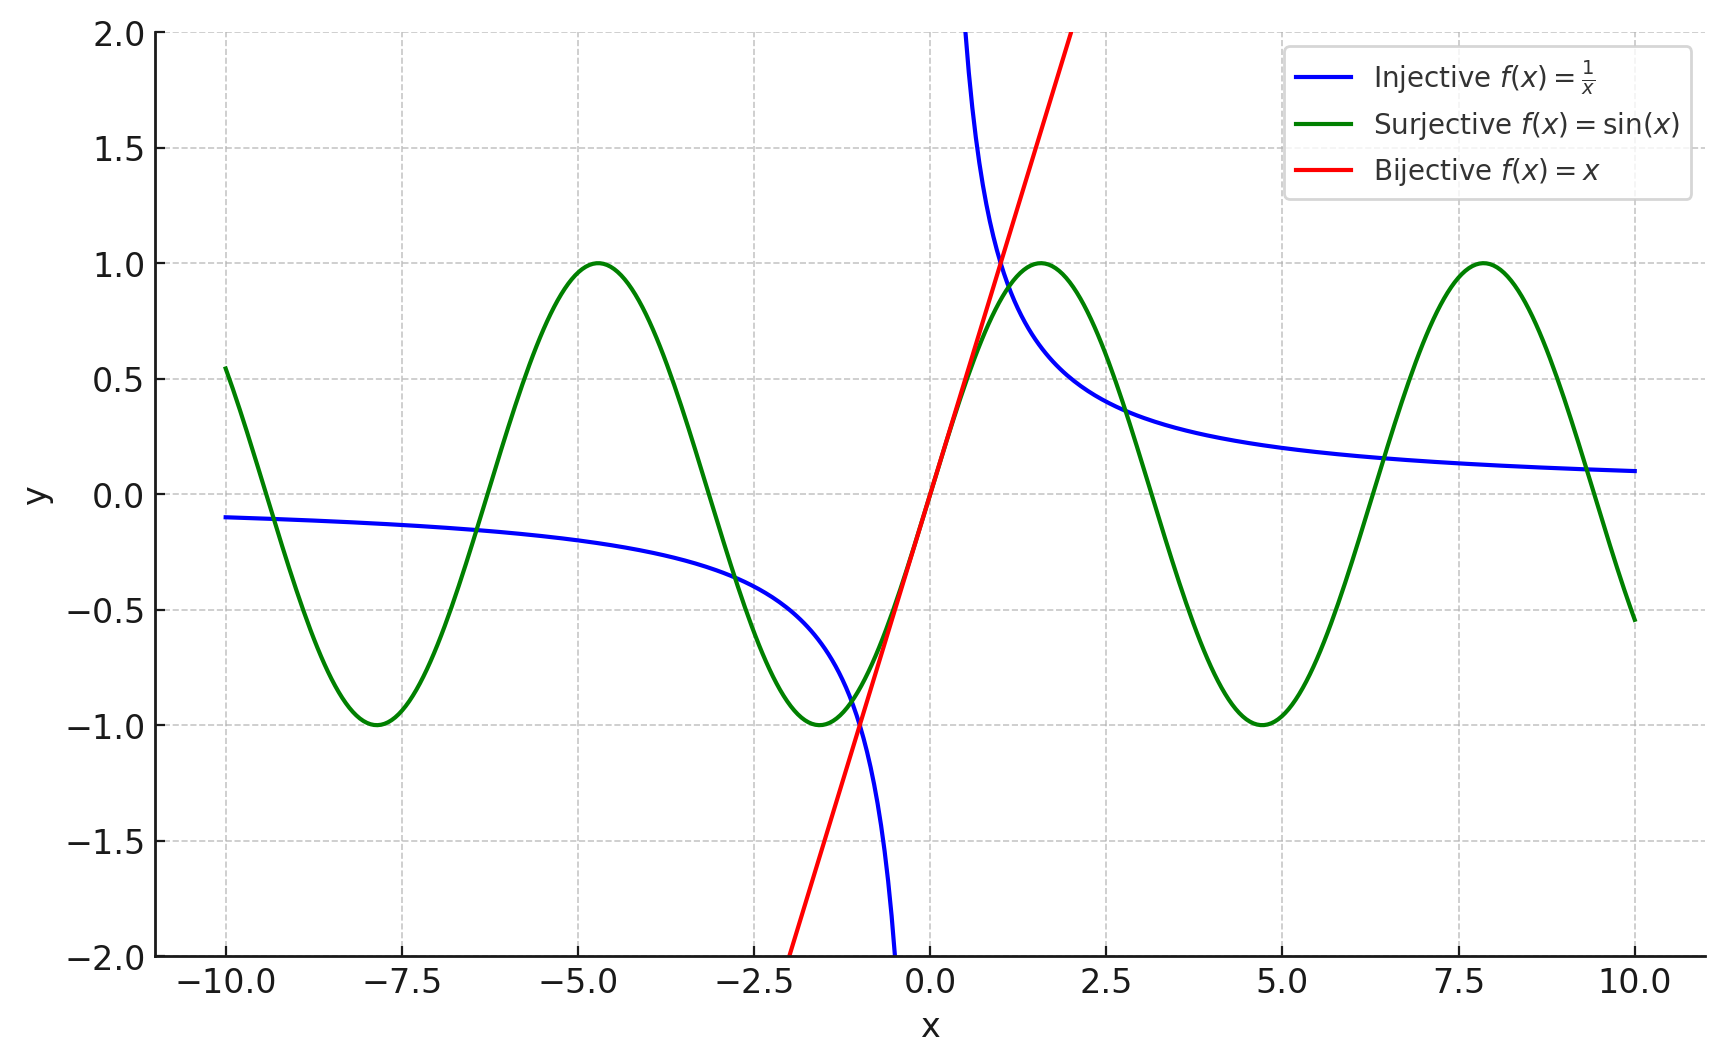
\includegraphics[width=0.75\linewidth]{Images/func.jpg}
    \caption{Examples of Special Mappings}
    \label{fig:fuc}
\end{figure}

Examine the figure \autoref{fig:fuc}, where one example of each type of function is shown. Fundamentally, when we define these functions, only two properties are involve:
\begin{itemize}
    \item A: It the mapping retrievable? (for every value in the image, we can find where it is from without any confusion.
    \item B: Is the mapping is full comparing to the preimage?(Whether every value in the preimage has a mapping to the image)
\end{itemize}
If A is satisfied, we call it injective function.

If B is satisfied, we call it surjective function.

If both A and B are satisfied, we say the function is bijective.

Using $A$, $B$, and $C$ to denote the set of injective, surjective, and bijective function respectively, it is therefore that :

    $$A\cap B = C$$

Which means that if a function is injective and surjective in the same time, it is bijective. 

And these will be all we need to know about function for now, since the rest of the properties will be discussed in single-variable calculus. This section aims only introduce the idea of injectivity, surjectivity, and bijectivity, 

\subsection{Exercises}
\begin{exercise}
    Determine the images of the functions \( f: \mathbb{R} \rightarrow \mathbb{R} \) defined as follows:
    \begin{enumerate}
        \item[a)] \( f(x) = \frac{x^2}{1 + x^2} \).
        \item[b)] \( f(x) = \frac{x}{1 + |x|} \).
    \end{enumerate}
\end{exercise}
\begin{proof}[Solution for a)]
    We analyze the function \( f(x) = \frac{x^2}{1 + x^2} \):
    \begin{itemize}
        \item This function is defined for all \( x \in \mathbb{R} \).
        \item For \( x = 0 \), \( f(0) = 0 \).
        \item For \( x \neq 0 \), \( f(x) \) is always positive.
        \item As \( x \) approaches infinity, \( f(x) \) approaches 1.
    \end{itemize}
    Thus, the image of \( f \) is \( (0, 1] \).
    \end{proof}
    
    \begin{proof}[Solution for b)]
    We analyze the function \( f(x) = \frac{x}{1 + |x|} \):
    \begin{itemize}
        \item This function is defined for all \( x \in \mathbb{R} \).
        \item For \( x > 0 \), as \( x \) increases, \( f(x) \) approaches 1.
        \item For \( x < 0 \), as \( x \) decreases, \( f(x) \) approaches -1.
    \end{itemize}
    Thus, the image of \( f \) is \( (-1, 1) \).
    \end{proof}



%------------------------------------------------
\section{Summation}
Before we move on to the most important part of this chapter, sequence, we use this section to introduce a prerequisite for studying its properties. We introduce the Sigma sign.

In earlier chapters, we have seen exercises such as finding the expression of the sum of the first nth positive integer:
$$1 + 2 + \dots + (n-1) + (n)= \frac{n(n+1)}{2}$$ 
From now on, we will use the sigma notation to deal with the summation of numbers. Such as:
\subsection{Sigma Notation}
\begin{notation}[Sigma Notation]
    \[
\sum_{i=1}^{n} i = \frac{n(n + 1)}{2}
    \]
\end{notation}
Where $i$ is quite similar to iterator, or sometimes we also call counter in programming languages, and $n$ refers to the condition of termination. The expression right after the sigma sign is called \textbf{summand}.

Actually, this is not the only way to express summation, it is also equivalent to:
\[\sum_{1\leq i\leq n} i = \frac{n(n+1)}{2}\]

Also, like what we do for set, we can also write sigma notation using description, such as: 
\[
\sum_{1 \leq k \leq 100} k^2
\]

\( k \) is odd

\subsection{Properties and Techniques of Sigma Notation}
This part of the section shows how we can handle summation expressions.
One of the greatest convenience of sigma notation is that every expression is adjustable, we can change the variable as what we prefer as in the following example.
\begin{example} \label{exp:siginvariance}
 \[
\sum_{1 \leq k \leq n} a_k = \sum_{1 \leq k+1 \leq n} a_{k+1}
\]
\end{example}
This technique has a significant effect to some mathematical proofs.
Another points to keep in mind is that: always make the expression simple in terms of upper and lower boundary.
\begin{example}
    Examine this expression: 
    \[\sum_{k=0}^{n} k(k-1)(k-n)\]
    The sum when k equals to 0, 1, and $n$ is 0. In this case we cannot say it is a good expression, as what we want is the sum it self, while 0 does not matter for us. Therefore, we just fine-tune it to:
    \[\sum_{k=2}^{n-1} k(k-1)(k-n)\]
    This makes it concise and clear.
\end{example}

\subsubsection{Manipulation of Sigma Notation}
For a set \( K \), the following summation properties hold. Let \( c \) be a constant, and \( a_k \), \( b_k \) be sequences indexed by \( K \):

\begin{equation}
    \sum_{k \in K} c a_k = c \sum_{k \in K} a_k \quad \text{(Distributive Law)}
    \label{eq:constant_factor}
\end{equation}

\begin{equation}
    \sum_{k \in K} (a_k + b_k) = \sum_{k \in K} a_k + \sum_{k \in K} b_k \quad \text{(Associative Law)}
    \label{eq:summation_of_sums}
\end{equation}

\begin{equation}
    \sum_{k \in K} a_k = \sum_{p(k) \in K} a_{p(k)} \quad \text{(Commutative Law, as in example \autoref{exp:siginvariance})} 
    \label{eq:permutation_invariance}
\end{equation}
The proof is attached below.

\textbf{Proof of Constant Factor Law:}

Let \( c \) be a constant and \( a_k \) be a sequence indexed by a finite set \( K \). We want to show that \( \sum_{k \in K} c a_k = c \sum_{k \in K} a_k \).

By the definition of summation and the distributive property of multiplication over addition, we have:
\begin{equation}
    \sum_{k \in K} c a_k = c a_1 + c a_2 + \ldots + c a_n = c (a_1 + a_2 + \ldots + a_n) = c \sum_{k \in K} a_k.
\end{equation}
This concludes the proof of the constant factor law.

\textbf{Proof of Summation of Sums Law:}

Let \( a_k \) and \( b_k \) be sequences indexed by a finite set \( K \). We want to show that \( \sum_{k \in K} (a_k + b_k) = \sum_{k \in K} a_k + \sum_{k \in K} b_k \).

By the definition of summation and the associative and commutative properties of addition, we have:
\begin{equation}
    \begin{split}
\sum_{k \in K} (a_k + b_k) &= (a_1 + b_1) + (a_2 + b_2) + \ldots + (a_n + b_n) \\
&= (a_1 + a_2 + \ldots + a_n) + (b_1 + b_2 + \ldots + b_n) \\
&= \sum_{k \in K} a_k + \sum_{k \in K} b_k
\end{split}
\label{eq:sum_of_sums}
\end{equation}
This concludes the proof of the summation of sums law.

\textbf{Proof of Permutation Invariance Law:}

Let \( a_k \) be a sequence indexed by a finite set \( K \). Let \( p: K \to K \) be a bijection, which means \( p \) permutes the indices. We want to show that \( \sum_{k \in K} a_k = \sum_{p(k) \in K} a_{p(k)} \).

By the definition of summation and the fact that addition is commutative (the order does not matter), we have:
\begin{equation}
    \sum_{k \in K} a_k = a_1 + a_2 + \ldots + a_n = a_{p(1)} + a_{p(2)} + \ldots + a_{p(n)} = \sum_{p(k) \in K} a_{p(k)}.
\end{equation}
This concludes the proof of the permutation invariance law.
\subsubsection{Multiple Sums}
Sometimes we use sigma notation with multiple variables, just like what we can do to write loops in programming languages.

    
$$\sum_{1 \leq j, k \leq 3} a_j b_k = a_1b_1 + a_1b_2 + a_1b_3 + a_2b_1 + a_2b_2 + a_2b_3 + a_3b_1 + a_3b_2 + a_3b_3 $$


In the context of summation, we often encounter a situation where a sum is taken over a set of pairs. Specifically, let \( P(j, k) \) be a property involving the indices \( j \) and \( k \), and \( a_{j,k} \) be elements corresponding to these indices. The summation over all pairs \( (j, k) \) satisfying property \( P \) is equivalent to summing over all indices separately:

\[
\sum_{P(j,k)} a_{j,k} = \sum_{j,k} a_{j,k} \cdot P(j,k).
\]

This notation serves as a shorthand for expressing the sum over a subset of indices determined by the property \( P \).
There are also cases where we must use two sigma notation in the same time.

 
\begin{example}[Double Summation]
    When considering a double sum over a set of pairs, we often come across the following identity:

\begin{equation}
\sum_{j}\sum_{k} a_{j,k} [P(j,k)]
\end{equation}

where \( [P(j,k)] \) is an Iverson bracket which equals 1 if the property \( P \) holds for the pair \( (j,k) \) and 0 otherwise.
\end{example}


By interchanging the order of summation, we observe that:

\begin{equation}
\sum_{j}\sum_{k} a_{j,k} [P(j,k)] = \sum_{k}\sum_{j} a_{j,k} [P(j,k)].
\end{equation}

This property allows us to switch the order of summation without changing the result, which can be particularly useful in various mathematical analyses.

Double summation could also be used to simplify a given summation.
Considering the expression at the beginning of this section:
$$\sum_{1 \leq j, k \leq 3} a_j b_k = a_1b_1 + a_1b_2 + a_1b_3 + a_2b_1 + a_2b_2 + a_2b_3 + a_3b_1 + a_3b_2 + a_3b_3 $$

\begin{example}[Converting to Double Summation]
    \[
\sum_{1 \leq i,j,k \leq 3} a_j b_k = \sum_{\substack{i,j,k \\ 1 \leq i,j,k \leq 3}} a_j b_k \left[1 \leq j \leq 3\right] \left[1 \leq k \leq 3\right]
\]
\[
= \sum_j \sum_k a_j b_k \left[1 \leq j \leq 3\right] \left[1 \leq k \leq 3\right]
\]
\[
= \sum_j a_j \left[1 \leq j \leq 3\right] \sum_k b_k \left[1 \leq k \leq 3\right]
\]
\[
= \sum_j a_j \left[1 \leq j \leq 3\right] \left( \sum_k b_k \left[1 \leq k \leq 3\right] \right)
\]
\[
= \left( \sum_j a_j \left[1 \leq j \leq 3\right] \right) \left( \sum_k b_k \left[1 \leq k \leq 3\right] \right)
\]
\[
= \left( \sum_{j=1}^3 a_j \right) \left( \sum_{k=1}^3 b_k \right).
    \]

\end{example}
To explicit:
In the situation where we perform the same range of summation over each variable, the first two lines' triple summation is:
\[
(a_1b_1 + a_1b_2 + a_1b_3) + (a_2b_1 + a_2b_2 + a_2b_3) + (a_3b_1 + a_3b_2 + a_3b_3).
\]
Utilizing the distributive property to combine the summation operations into one involving \( a \), since \( a \) and each \( k \) for \( 1 \leq j \leq 3 \) are independent, yields (as in the third line):
\[
a_1(b_1 + b_2 + b_3) + a_2(b_1 + b_2 + b_3) + a_3(b_1 + b_2 + b_3).
\]

Consider a double sum over two independent indices, if the indices are independent, the summation of the product can be split into the product of two summations. For instance, the sum of products of \(a_j\) and \(b_k\) over \(j\) in \(J\) and \(k\) in \(K\) can be expressed as: \( (a_1 + a_2 + a_3)(b_1 + b_2 + b_3) \). This can be generalized to an expression:

\begin{equation}
\sum_{j \in J} \sum_{k \in K} a_j b_k = \left( \sum_{j \in J} a_j \right) \left( \sum_{k \in K} b_k \right),
\end{equation}
which is known as the \textbf{general distributive law}.
\begin{remark}
    If you are an agile reader, you must have noticed that this expression is a kind of representation of Cartesian sets in algebra. The general distributive law allows the sum over a function of elements from the Cartesian product of two sets to be expressed as the product of sums over each set if the function is separable into independent factors.
\end{remark}
\subsection{Exercises}
\begin{exercise}
    Express the triple sum
\[
\sum_{1 \leq i < j < k \leq 4} a_{ijk}
\]
as a three-fold summation (with three \(\sum\)'s), 

\begin{enumerate}[label=\alph*.]
    \item summing first on \( k \), then \( j \), then \( i \);
    \item summing first on \( i \), then \( j \), then \( k \).
\end{enumerate}
Also write your triple sums out in full without the \(\sum\)-notation, using parentheses to show what is being added together first.
\end{exercise}
\textbf{Solution:}

\textbf{(a)} \[
\sum_{i=1}^{4} \sum_{j=i+1}^{4} \sum_{k=j+1}^{4} a_{ijk} = 
\sum_{i=1}^{2} \sum_{j=i+1}^{3} \sum_{k=j+1}^{4} a_{ijk} = 
((a_{123} + a_{124}) + a_{134}) + a_{234}.
\]

\textbf{(b)} \[
\sum_{k=1}^{4} \sum_{j=1}^{k-1} \sum_{i=1}^{j-1} a_{ijk} = 
\sum_{k=3}^{4} \sum_{j=2}^{k-1} \sum_{i=1}^{j-1} a_{ijk} = 
a_{123} + (a_{124} + a_{134} + a_{234}).
\]

\begin{exercise}
    Demonstrate your understanding of \(\Sigma\)-notation by writing out the sums
\[
\sum_{k=0}^{5} a_k \quad \text{and} \quad \sum_{0\leq k^2 \leq 5} a_{k^2}
\]
in full. (Watch out—the second sum is a bit tricky.)

\end{exercise}
\textbf{Solution:}

The first sum is:
\[
a_0 + a_1 + a_2 + a_3 + a_4 + a_5
\]

The second sum, being tricky, $k \in \{-2, -1, 0, 1, 2\}$, therefore:
\[
a_4 + a_1 + a_0 + a_1 + a_4
\]

\begin{exercise}
    The general rule for summation by parts is equivalent to
\[
\sum_{0 \leq k < n} (a_{k+1} - a_k)b_k = a_nb_n - a_0b_0 - \sum_{0 \leq k < n} a_{k+1}(b_{k+1} - b_k), \quad \text{for } n \geq 0.
\]

Prove this formula by using the distributive, associative, and commutative laws.
\end{exercise}
Hint: Use Associative Law to LHS, try to make the indices of the two sums as similar as possible.
\begin{proof}
    \begin{align*}
        \text{LHS} &= \sum_{0\leq k < n} a_k b_{k+1} - \sum_{0\leq k < n} a_k b_k \\
        &= \sum_{0\leq k < n} a_k b_{k+1} - \sum_{-1\leq k < n-1} a_{k+1} b_{k+1} \\
        &= \sum_{0\leq k < n} a_k b_{k+1} - \sum_{0\leq k < n-1} a_{k+1} b_{k+1} \\
        &= \sum_{k=0}^{n-1} a_k b_{k+1} - \sum_{k=0}^{n-2} a_{k+1} b_{k+1} \\
        &= a_n b_{n-1} - a_0 b_0 + \sum_{k=0}^{n-2} a_k b_k - \sum_{k=0}^{n-2} a_{k+1} b_{k+1} \\
        &= a_n b_{n-1} - a_0 b_0 + \sum_{0\leq k < n-1} a_k (b_k - b_{k+1}) \\
        &= a_n (b_n - b_{n-1}) + a_n b_{n-1} - a_0 b_0 - \sum_{0\leq k < n-1} a_{k+1} (b_{k+1} - b_k) \\
        &= a_n (b_n - b_{n-1} + b_{n-1}) - a_0 b_0 - \sum_{0\leq k < n} a_{k+1} (b_{k+1} - b_k) \\
        &= a_n b_n - a_0 b_0 - \sum_{0\leq k < n} a_{k+1} (b_{k+1} - b_k) \\
        &= \text{RHS}
        \end{align*}
\end{proof}
\begin{exercise}
    Is the following expression correct or not? Give your reason.
    \[
\left( \sum_{i=1}^{n} a_i \right) \left( \sum_{j=1}^{n} \frac{1}{a_j} \right) = \sum_{1 \leq i \leq n} \sum_{1 \leq j \leq n} \frac{a_i}{a_j} = \sum_{1 \leq i \leq n} \sum_{1 \leq i \leq n} \frac{a_i}{a_i} = \sum_{i=1}^{n} 1 = n
\]
\end{exercise}
Consider the expression given by:
\[
\left( \sum_{i=1}^{n} a_i \right) \left( \sum_{j=1}^{n} \frac{1}{a_j} \right)
\]
and its expansion into a double sum:
\[
\sum_{1 \leq i \leq n} \sum_{1 \leq j \leq n} \frac{a_i}{a_j}
\]

It is claimed that this is equal to:
\[
\sum_{1 \leq i \leq n} \sum_{1 \leq i \leq n} \frac{a_i}{a_i} = \sum_{i=1}^{n} 1 = n
\]

However, this claim overlooks the fact that the double sum includes terms where \( i \neq j \), which are not necessarily equal to 1. Only when \( i = j \) does the term \( \frac{a_i}{a_j} \) simplify to 1, contributing to the count of \( n \).

Hence, the proper expansion of the double sum should be written as:
\[
\sum_{i=1}^{n} \sum_{j=1}^{n} \frac{a_i}{a_j} = \sum_{i=1}^{n} 1 + \sum_{\substack{i,j=1 \\ i \neq j}}^{n} \frac{a_i}{a_j}
\]
where the first sum on the right-hand side counts the \( n \) instances where \( i = j \), and the second sum accounts for the \( n(n-1) \) instances where \( i \neq j \).

The claim would only be true if all \( a_i \) are equal, which is a special case, not the general case. In the general case, the expression evaluates to something different than \( n \) due to the presence of terms where \( i \neq j \). 

Therefore, the original statement is incorrect unless the condition that all \( a_i \) are equal is specified.
%------------------------------------------------

\section{Sequence}
If everything so far is not a problem for you, congratulations, because you have known everything you need to know sequence. Sequence is an important concept that will be used throughout your journey of learning math. A Sequence
is defined as:
\begin{definition}
    A sequence is a function \( f: \mathbb{N} \to \mathbb{R} \), where \(\mathbb{N}\) is the set of natural numbers and \(\mathbb{R}\) is the set of real numbers. The value \( f(n) \) 
    is the \( n \)-th term of the sequence, often denoted as \( a_n \). Therefore, a sequence can be represented as \( \{a_n\}_{n=1}^{\infty} \) for an infinite sequence or \( \{a_n\}_{n=1}^{N} \) for a finite sequence of length \( N \).
\end{definition} 

\subsection{Introduction}
Sequences could be either infinite or finite. A \textit{sequence} is defined to be a function \( S \) whose domain \( D \) is a nonempty interval of integers. \( S \) is an \textit{infinite sequence} if \( D \) has the form \( \{a..\} \). % Usually \( a \) is 1 or 0.

\( S \) is a \textit{finite sequence} if \( D \) has the form \( \{a..b\} \) where \( a \leq b \). When \( |D| = n \), we will say that \( S \) is an \( n\text{-sequence} \). We will take the domain of an \( n\text{-sequence} \) to be the set \( \{1..n\} \). % But \( a \) could be 0, and then \( D \) is \( \{0..(n - 1)\} \).

The (natural) ordering of the domain of a sequence \( S \) gives a natural ordering to the ordered pairs in the set \( S \). If \( S \) is a 5-sequence, then
\[ S = \{(1, S(1)), (2, S(2)), (3, S(3)), (4, S(4)), (5, S(5))\} \]

\begin{example}
    Suppose \( D = \{1..10\} \), and we define the function \( S \) on \( D \) by

\[ S(i) = \text{the smallest prime factor of the integer } (1 + i). \]

Then \( D \) is a finite interval of integers, and so \( S \) is the sequence denoted by

\[ S = (2, 3, 2, 5, 2, 7, 2, 3, 2, 11). \]
\end{example}

\begin{definition}[Sum of Sequence]
    If \( S = (S_1, S_2, S_3, \ldots, S_n) \) is a finite sequence of numbers, the corresponding \textit{series} is the sum of the entries in \( S \)
    is:

\[ S_1 + S_2 + S_3 + \ldots + S_n. \]
\end{definition}
\subsection{Special Sequences}
This section introduces common sequences as well as their properties.
\subsubsection{Algorithmic Sequence}
Algorithmic sequences are a fundamental concept in both computer science and mathematics, forming the backbone of algorithm design and analysis. These sequences are typically defined as an ordered set of steps or instructions, aimed at solving a specific problem or accomplishing a particular computation.
\begin{definition}[Arithmetic Sequence]
    An arithmetic sequence of the form
\[
a, a + d, a + 2d, \ldots, a + nd, \ldots
\]
where the initial term \( a \) and the common difference \( d \) are real numbers.
\end{definition}
Usually, the notation $a_n$ is used to express the nth term of a sequence (starting from 0). For the example in the 
definition, we have $a_0 = a$ and $a_n = a_0 + nd$. 
We also have:
$$a_1 = a_0 + d$$
$$a_2 = a_1 + d$$
$$\dots$$
$$a_n = a_0 + nd$$ 
for $n>=1$, $n\in \mathbb{Z}$:
$$a_n = a_{n-1} + d$$
These formula shows the linking between consecutive terms in an arithmetic sequence. We know that the sum
$s$ of the sequence is:
\begin{align*}
    S & =\ a_{0} \ +\ a_1\ \ +\ \dotsc \ +\ a\_n\\
    S & =\ a_{0} \ +\ a_{0} +d\ +\ \dotsc \ +\ a_{n-1} +d
    \end{align*}
The sum is expressed in infinite terms, and it is called \textbf{open form equation}. Accordingly, there are also \textbf{closed form
equations}.
\begin{definition}[Open Form]
    An \textit{open form} or \textit{non-closed form} expression, on the other hand, does not have a finite standard representation and often requires recursive or iterative methods for evaluation. It may involve summations, integrals, or other operations that are not easily simplified into a finite number of operations.
\end{definition}
\begin{definition}[Closed Form]
    A \textit{closed form} expression is a mathematical expression that can be evaluated in a finite number of standard operations. It typically involves constants, variables, and operations from algebra, calculus, and other areas of mathematics that can be computed in a finite number of steps.
    A closed form expression provides a direct way to compute the term of a sequence without the need for recursion.
\end{definition}

Is the open form good for calculating the sum of a sequence? Suppose now I want to know $S_{100}$ (The sum of the first 100th terms),
with the open form, I still have to calculate 99 terms using the definition of this sequence. So is there a way 
to make it possible that we get the sum in one step? Think about closed form. The closed form allows us to calculate
the sum directly. But is it possible to transform an open expression to closed form? If possible, how?

You may already notice that the open form has a property of infinity, and each step is somewhat related.
Isn't it a perfect problem to be solved by mathematical induction? We will leave this proof as a exercise, and here we provide another direct proof
by the symmetry of arithmetic sequence.
\begin{theorem}[Sum of Arithmetic Sequence]
    For  arithmetic sequence \( a_0, a_1, \ldots, a_{n-1} \), where each term can be expressed as \( a_i = a_0 + id \) and \( d \) is the common difference. The sum of the first nth terms is:
    \[ S = \frac{n}{2}[2a_0 + (n-1)d] \] or \[ S = \frac{n}{2}(a_0 + a_{n-1}) \] where \[ a_n = a_0 + nd \]
\end{theorem}
\begin{remark}
    We are trying to find the sum of the first n terms, and the first term is $a_0$, so the last term is
    $a_{n-1}$.
\end{remark}
\begin{proof}
    Consider an arithmetic sequence \( a_0, a_1, \ldots, a_n \), where each term can be expressed as \( a_i = a_0 + id \) and \( d \) is the common difference.
    \item Write the sum of the sequence in order:
\[
S = a_0 + (a_0 + d) + (a_0 + 2d) + \ldots + (a_0 + (n-1)d)
\]

\item Write the sum of the sequence in reverse order:
\[
S = (a_0 + (n-1)d) + (a_0 + (n-2)d) + \ldots + a_0
\]

\item Add these two equations together, every pair of terms within the brackets forms: \[ 2a_0 + (n-1)d \]

\item Since each term appears in a pair, there are \( n \) such pairs.

\item The resulting equation is \( 2S = n[2a_0 + (n-1)d] \).

\item Solving for \( S \) gives us \( S = \frac{n}{2}[2a_0 + (n-1)d] \) or \( S = \frac{n}{2}(a_0 + a_n) \), where \( a_n = a_0 + (n-1)d \).
\end{proof}


\subsubsection{Geometric Sequence}
Geometric sequence is the other important and common sequence that involved in problem-solving of computer
Science. 
A geometric sequence, also known as a geometric progression, is a sequence of numbers where each term after 
the first is found by multiplying the previous term by a fixed, non-zero number called the common ratio. 
Mathematically, a geometric sequence is defined as follows:
\begin{definition}[Geometric Sequence]
    Given the first term \( a_0 \) (also referred to as \( a_1 \) in some texts) and the common ratio \( r \), the \( n \)-th term of a geometric sequence \( a_n \) can be expressed as:
\[
a_n = a_0 \cdot r^n \quad \text{for } n \geq 0
\]
where \( n \) is a non-negative integer representing the position of the term in the sequence.
\end{definition}    

The common ratio \( r \) can be any real number. If \( |r| < 1 \), the terms of the sequence 
will get progressively smaller and approach zero. If \( |r| > 1 \), the terms will grow progressively 
larger. If \( r = 1 \), the sequence is constant, and if \( r = -1 \), the sequence will alternate 
between two values.

We can deduce the sum of a specific geometric sequence by direct proof.
\begin{theorem}[Sum of Geometric Sequence]
    
\end{theorem}

\begin{proof}
    Consider a geometric sequence with the first term \( a_0 \) and the common ratio \( r \) where \( r \neq 1 \). The sequence is given by:
\[ a_0, a_0r, a_0r^2, \ldots, a_0r^{n-1} \]

The sum of the first \( n \) terms of the sequence, denoted by \( S_n \), is:
\[ S_n = a_0 + a_0r + a_0r^2 + \ldots + a_0r^{n-1} \]

To find a formula for \( S_n \), multiply the entire sequence by \( r \):
\[ rS_n = a_0r + a_0r^2 + a_0r^3 + \ldots + a_0r^n \]

Subtract the original sum \( S_n \) from this new sum \( rS_n \) to get a telescoping series:
\[ rS_n - S_n = a_0r^n - a_0 \]

Solving for \( S_n \) gives us:
\[ S_n = \frac{a_0(1 - r^n)}{1 - r} = \]

This is the sum formula for the first \( n \) terms of a geometric sequence when \( r \neq 1 \). If \( r = 1 \), the sequence is constant, and the sum of the first \( n \) terms is simply \( n \) times the first term \( a_0 \).
\end{proof}
%----------------------------------------------------------------------
\subsubsection{characteristic Sequence}
\begin{definition}[Characteristic Sequence]
    Suppose that \( U \) is some given \( n \)-set whose elements have been \textit{indexed} (listed in a certain order) so that \( U = \{x_1, x_2, \ldots, x_n\} \). If \( A \) is a subset of \( U \), the \textit{characteristic sequence} of \( A \) is the function whose domain is \( \{1..n\} \) defined by

\[
X^A_i = X^A(i) = 
\begin{cases} 
1 & \text{if } x_i \in A \\
0 & \text{if } x_i \notin A 
\end{cases}
\]
\end{definition}

\begin{example}
    If \( U \) is the set of the first 10 odd positive integers, \( A \) is the subset of primes in \( U \), and \( B \) is the set of multiples of 3 in \( U \), then
    
    \[
    \begin{aligned}
    &U = \{1, 3, 5, 7, 9, 11, 13, 15, 17, 19\} &&// x_i = 2i - 1. \\
    &A = \{3, 5, 7, 11, 13, 17, 19\} \\
    &B = \{3, 9, 15\} \\
    &X^A = (0, 1, 1, 1, 0, 1, 1, 0, 1, 1) \\
    &X^B = (0, 1, 0, 0, 1, 0, 0, 1, 0, 0).
    \end{aligned}
    \]
    \end{example}

    Characteristic sequences may be used as an implementation model for subsets of any given indexed set \( U \). The set operations may be done on these sequences:
    \[
    X^{A \cap B}_i = X^A_i \times X^B_i;
    \]
    \[
    X^{A \cup B}_i = X^A_i + X^B_i - X^A_i \times X^B_i;
    \]
    \[
    X^{A \setminus B}_i = X^A_i - X^A_i \times X^B_i.
    \]
    
    If \( A \subseteq B \) then
    \[
    X^A_i \leq X^B_i \quad \text{for each index } i,
    \]
    and
    \[
    |A| = \sum_{i=1}^{n} X^A_i.
    \]

%----------------------------------------------------------------------
\subsection{Exercises}
\begin{exercise}
    Find the sum of arithmetic sequence using mathematical induction. Try \textbf{NOT} use the conclusion in this section.
\end{exercise}
Hint: Consider the sum of the first nth positive integer. Try to make assumption by taking it as an arithmetic sequence.
\begin{proof}
    Let \( S(n) \) denote the sum of the first \( n \) terms of an arithmetic sequence with the first term \( a_0 \) and common difference \( d \).
    \begin{itemize}
        \item \textbf{Base Case (\( n = 1 \))}: The sum of the sequence with only the first term is the first term itself, \( S(1) = a_0 \).
        \item \textbf{Inductive Step}: Assume that the sum of the first \( k \) terms \( S(k) \) is given by a certain formula. We want to show that the sum of the first \( k+1 \) terms \( S(k+1) \) can be expressed using the same formula.
        \end{itemize}
        
        For the base case, we can easily see that:
        \[
        S(1) = a_0
        \]
        As $\sum_{1}^{n}i = \frac{n(n+1)}{2}$, which could be taken as an arithmetic sequence with $a_0=1$ and
        $a_n=n$.
        By this, assume that the sum of the first \( k \) terms is:
        \[
        S(k) = \frac{k}{2} [a_0 + a_n]
        \]
        equivalent to
        \[
        S(k) = \frac{k}{2} [2a_0 + (k-1)d]
        \]
        
        To prove the inductive step for \( S(k+1) \), consider:
        \[
        S(k+1) = S(k) + a_0 + kd
        \]
        
        Substituting the inductive hypothesis into the above equation yields:
        \[
        S(k+1) = \frac{k}{2} [2a_0 + (k-1)d] + a_0 + kd
        \]
        
        After simplifying, we aim to show that:
        \[
        S(k+1) = \frac{k+1}{2} [2a_0 + kd]
        \]
        
        This will complete the proof if we can establish that the simplified version of \( S(k+1) \) matches the form of the inductive hypothesis.
\end{proof}
\begin{exercise}
    Prove the sum of geometric sequence  is \( S_n = \frac{a_0(1 - r^n)}{1 - r} = \) using mathematical induction.
\end{exercise}
\begin{proof}
    We want to prove that the sum of the first \( n \) terms of a geometric sequence \( S_n \) with the first term \( a \) and common ratio \( r \) (where \( r \neq 1 \)) is given by:

\[ S_n = \frac{a(1 - r^n)}{1 - r} \]

\textbf{Base Case (n=1):}

The sum of the first term is simply the term itself:

\[ S_1 = a \]

which agrees with the formula.

\textbf{Inductive Step:}

Assume the formula holds for \( n = k \), that is,

\[ S_k = \frac{a(1 - r^k)}{1 - r} \]

We need to prove that it also holds for \( n = k+1 \):

\[ S_{k+1} = \frac{a(1 - r^{k+1})}{1 - r} \]

Starting with the inductive hypothesis for \( S_k \) and adding the \( (k+1) \)-th term \( ar^k \) to both sides, we have:

\[ S_k + ar^k = \frac{a(1 - r^k)}{1 - r} + ar^k \]

Simplifying, we obtain:

\[ S_{k+1} = S_k + ar^k = \frac{a - ar^{k+1}}{1 - r} \]

which is the same as the formula for \( S_{k+1} \), thus completing the proof.
\end{proof}
\begin{exercise}
    Given a sequence \( \{a_n\} \) and a series \( S_n = an^2 + bn + c (a \neq 0) \).

\begin{enumerate}
    \item Find the general term \( a_n \);
    \item Is the sequence \( \{a_n\} \) an arithmetic sequence?
\end{enumerate}
\end{exercise}
Hint: How can we get the value of a term from the sum of a sequence?
\textbf{Solution:}

\begin{enumerate}
    \item For \( n \geq 2 \), \( a_n = S_n - S_{n-1} = (an^2 + bn + c) - [a(n-1)^2 + b(n-1) + c] \) \\
    \( = (b+a) + (n-1) \cdot 2a \),
    
    Therefore, for \( n=1 \), \( a_1 = (b+a) + (1-1) \cdot 2a = b + a + c - S_1 \), \\
    and the general term is
    \[
    a_n = 
    \begin{cases}
        a + b + c & (n=1) \\
        (b+a) + (n-1) \cdot 2a & (n \geq 2)
    \end{cases}
    \]

    \item Since \( c = 0 \), \( a_n \) can be simplified to \( a_n = a + b \), which is constant and equals \( 2a \) when \( n \geq 2 \). This implies \( \{a_n\} \) is an arithmetic sequence with common difference \( 2a \), provided \( a, b \) are constants and \( a \neq 0 \).
    
    Note: From \( S_n \) we can deduce \( a_n = S_n - S_{n-1} \) when \( n \geq 2 \). Since \( a_1 = S_1 \), the sequence \( a_n = S_n - S_{n-1} \) (for \( n \geq 2 \)) and \( a_1 \) is the first term. The sequence \( \{a_n\} \) is an arithmetic sequence.
    
    Therefore, the general term \( a_n \) can be expressed as:
    \[
    a_n = 
    \begin{cases}
        S_1 & (n=1) \\
        S_n - S_{n-1} & (n \geq 2)
    \end{cases}
    \]
    
    Given the series \( \{a_n\} \) with \( S_n = an^2 + bm + c (a \neq 0) \), the sequence \( \{a_n\} \) is an arithmetic sequence with common difference \( 2a \) when \( c = 0 \).
\end{enumerate}

\begin{exercise}
    Given constants $a$, $b$, $c$, consider the sum $S_n = 1^2 + 2^2 + 3^2 + \ldots + n(n+1)^2 = \frac{n(n+1)}{12}(an^2 + bn + c)$, where $an^2 + bn + c \neq 0$.
\end{exercise}
\begin{proof}
    For $n=1$, we have $\frac{1}{6}(a+b+c)$, thus $a_1 = 4 = \frac{1}{6}(a+b+c)$.
For $n=2$, we have $\frac{22}{2} = 11 = \frac{1}{2}(4a+b+c)$, thus $a_2 = 22 = 9a + 3b + c$.
For $n=3$, $a_3 = 70 = 9a + 3b + c$.\\

From these equations, we find that:
\begin{align*}
    a + b + c &= 24 \\
    4a + b + c &= 44 \\
    9a + 3b + c &= 70
\end{align*}

Solving the system, we get $a=3$, $b=11$, $c=10$.
For \(n = 1, 2, 3\), the sum can be expressed as:
\[
1 \cdot 2^2 + 2 \cdot 3^2 + \ldots + n(n+1)^2 = \frac{n(n+1)}{12}(3n^2 + 11n + 10),
\]
thus, \(S_n = 1 \cdot 2^2 + 2 \cdot 3^2 + \ldots + n(n+1)^2\).

For a general term \(k\), \(S_k = \frac{k(k+1)}{12}(3k^2 + 11k + 10)\). Therefore,
\[
S_{k+1} = S_k + (k+1)(k+2)^2
\]
\[
= \frac{k(k+1)}{12}(3k^2 + 11k + 10) + (k+1)(k+2)^2
\]
\[
= \frac{k(k+1)}{12}((k+2)(3k+5) + (k+1)(k+2)^2)
\]
\[
= \frac{(k+1)(k+2)}{12}(3k^2 + 5k + 12k + 24)
\]
\[
= \frac{(k+1)(k+2)}{12}(3(k+1)^2 + 11(k+1) + 10).
\]

Hence, by induction, we can show that for \(n = k+1\) the sum is valid.

Finally, with \(a = 3\), \(b = 11\), \(c = 10\), we confirm that the given sequence is indeed a second-order arithmetic sequence.
\end{proof}

\begin{exercise}
    Evaluate:
    \begin{enumerate}
        \item $S = \sum_{1}^{n} \frac{N}{2^n}$
        \\
        \item $S = \sum_{1}^{n} \frac{3n-2}{5^{n-1}}$  
    \end{enumerate}
\end{exercise}

\textbf{Solution:}

(1) Given the series \( S_n = \frac{1}{2} + \frac{2}{4} + \frac{3}{8} + \cdots + \frac{n}{2^n} \), we can write:

\[
S_n - \frac{1}{2}S_n = \frac{1}{2} + \frac{1}{4} + \frac{1}{8} + \cdots + \frac{1}{2^n} - \frac{n}{2^{n+1}}
\]

This simplifies to:

\[
\frac{1}{2}S_n = \frac{1}{2} \left(1 - \left(\frac{1}{2}\right)^n\right) = \frac{1}{2} - \frac{1}{2^{n+1}} = \frac{1}{2} - \frac{n}{2^{n+1}} + \frac{n}{2^{n+1}}
\]

Hence, the series sum is:

\[
S_n = 2 - \frac{1}{2^{n-1}} - \frac{n}{2^n} = 2 - \frac{n+2}{2^n}
\]

(2) Considering the series \( S_n = 1 + \frac{4}{5} + \frac{7}{25} + \cdots + \frac{3n-2}{5^{n-1}} \), we proceed similarly:

\[
\left(1 - \frac{1}{5}\right)S_n = 1 + \frac{3}{5} + \frac{3}{25} + \cdots + \frac{3}{5^{n-1}} - \frac{3n-2}{5^n}
\]

The terms form a geometric series, so we get:

\[
S_n = 1 + \frac{3}{5} \left(1 + \frac{1}{5} + \frac{1}{25} + \cdots + \frac{1}{5^{n-2}}\right) - \frac{3n-2}{5^n}
\]

Applying the formula for the sum of a geometric series, we find:

\[
S_n = 1 + \frac{3}{5} \left(\frac{1 - \left(\frac{1}{5}\right)^{n-1}}{1 - \frac{1}{5}}\right) - \frac{3n-2}{5^n}
\]

Simplifying, we obtain:

\[
S_n = 1 + \frac{3}{5} \left(\frac{5^n - 5}{4 \cdot 5^{n-1}}\right) - \frac{3n-2}{5^n}
\]

Further simplification gives us:

\[
S_n = \frac{35}{16} - \frac{12n+7}{16 \cdot 5^{n-1}}
\]
%------------------------------------------------

\chapterimage{chap2.png} % Chapter heading image
\chapterspaceabove{5.75cm} % Whitespace from the top of the page to the chapter title on chapter pages
\chapterspacebelow{10cm} % Amount of vertical whitespace from the top margin to the start of the text on chapter pages
\chapter{Algorithm and Number}

Computer Science is most commonly known as an engineering subject, while the unanimous pursuit of all engineering subjects are solving problems. This chapter delves in to methods to solve problems, which is also known as \textbf{algorithm}. In the world of Computer Science, everything is proceeded in a methodical manner, and the very dependency of this is algorithm. Meanwhile, we will introduce pseudocode, one of the most important tools for algorithm analysis, as well as the representation of number in Computer Science.

%------------------------------------------------

\section{Numbers}
Every reader could be quite surprised when seeing the title for this section. Yes, numbers, we have known what is number since the very beginning when we get to learn math as toddlers. In this section, we will explain the system of number, not only will we figure out how numbers and their operations are defined, but how they are categorized.
\subsection{Typology of Numbers}
This part recalls the type of numbers we've learned since primary school and their set notations.
\label{sec:number}
\begin{enumerate}
  \item \textbf{Natural Numbers}
  \begin{itemize}
    \item Definition: Natural numbers are the set of positive integers used for counting and ordering, which do not include zero or negative numbers.
    \item Set Notation:
    \[
    \mathbb{N} = \{1, 2, 3, \ldots\}
    \]
  \end{itemize}

  \item \textbf{Integers}
  \begin{itemize}
    \item Definition: Integers are all the whole numbers including positive natural numbers, their negatives, and zero.
    \item Set Notation:
    \[
    \mathbb{Z} = \{\ldots, -3, -2, -1, 0, 1, 2, 3, \ldots\}
    \]
  \end{itemize}

  \item \textbf{Rational Numbers}
  \begin{itemize}
    \item Definition: Rational numbers are numbers that can be expressed as the quotient of two integers, a fraction \( \frac{a}{b} \), where \( a \) and \( b \) are integers and \( b \neq 0 \). The set includes all integers and fractions.
    \item Set Notation:
    \[
    \mathbb{Q} = \left\{\frac{a}{b} \mid a, b \in \mathbb{Z}, b \neq 0\right\}
    \]
  \end{itemize}

  \item \textbf{Irrational Numbers}
  \begin{itemize}
    \item Definition: Irrational numbers are real numbers that cannot be expressed as a ratio of two integers. The decimal expansion of irrational numbers is non-terminating and non-repeating. Examples include \(\pi\) and \(\sqrt{2}\).
    \item Set Notation:
    \[
    \mathbb{I} = \{x \in \mathbb{R} \mid x \notin \mathbb{Q}\}
    \]
    (Note: \(\mathbb{I}\) is used here for illustrative purposes and is not a standard symbol.)
  \end{itemize}

  \item \textbf{Real Numbers}
  \begin{itemize}
    \item Definition: The real numbers include both rational and irrational numbers, encompassing all points on an infinitely extended number line. The set of real numbers is continuous and is composed of all limits of sequences of rational numbers.
    \item Set Notation:
    \[
    \mathbb{R} = \{x \mid x \text{ is a limit of a sequence of rational numbers}\}
    \]
  \end{itemize}

  \item \textbf{Prime Numbers}
\begin{itemize}
  \item Definition: A prime number is a natural number greater than 1 that has no positive divisors other than 1 and itself. In other words, \( p \) is prime if \( p > 1 \) and if \( p \) is divisible only by 1 and \( p \).
  \item Set Notation:
  \[
  \mathbb{P} = \{p \in \mathbb{N} \mid p > 1 \text{ and } p \text{ has no divisors other than } 1 \text{ and } p\}
  \]
  \item Examples: The first few prime numbers are:
  \[
  2, 3, 5, 7, 11, 13, 17, \ldots
  \]
\end{itemize}
The following Venn diagram shows the relationship between different number sets.
\begin{figure}[H]
    \centering
    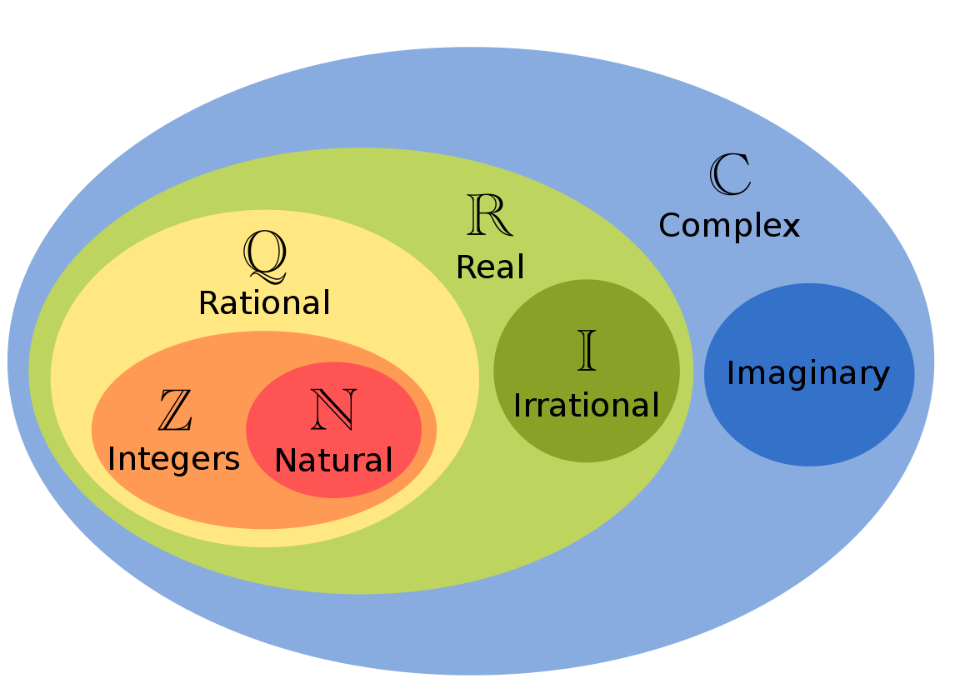
\includegraphics[width=0.5\linewidth]{venn.png}
    \caption{Venn Diagram of Number Sets}
    \label{venn}
\end{figure}

\begin{remark}
    Complex number is currently not a something necessary, as our discussion so far only falls in the real number set.
\end{remark}

\subsection{The Real Number System}
Considering the real numbers are the only system involved so far this book, here, we provide a new mathematical perspective that is different what we were taught, to understand the real number system. We will introduce three axioms that real number holds.
\begin{definition}[Field Axioms]\label{axi:field}
A set \( S \) with operations \( + \) and \( \cdot \) and distinguished elements 0 and 1 with \( 0 \neq 1 \) is a \emph{field} if the following properties hold for all \( x, y, z \in S \):

\begin{itemize}
  \item[A0:] \( x + y \in S \) \hfill Closure
  \item[A1:] \( (x + y) + z = x + (y + z) \) \hfill Associativity
  \item[A2:] \( x + y = y + x \) \hfill Commutativity
  \item[A3:] \( x + 0 = x \) \hfill Identity
  \item[A4:] given \( x \), there is a \( w \in S \) such that \( x + w = 0 \) \hfill Inverse
  \item[M0:] \( x \cdot y \in S \) \hfill Closure
  \item[M1:] \( (x \cdot y) \cdot z = x \cdot (y \cdot z) \) \hfill Associativity
  \item[M2:] \( x \cdot y = y \cdot x \) \hfill Commutativity
  \item[M3:] \( x \cdot 1 = x \) \hfill Identity
  \item[M4:] for \( x \neq 0 \), there is a \( w \in S \) such that \( x \cdot w = 1 \) \hfill Inverse
  \item[DL:] \( x \cdot (y + z) = x \cdot y + x \cdot z \) \hfill Distributive Law
\end{itemize}

\end{definition}
The operations \( + \) and \( \cdot \) are called addition and multiplication. The elements 0 and 1 are the additive identity element and the multiplicative identity element, respectively.   


It follows from these axioms that the additive inverse and multiplicative inverse (of a nonzero \( x \)) are unique. The additive inverse of \( x \) is the \textbf{negative} of \( x \), written as \( -x \). To define subtraction of \( y \) from \( x \), we let \( x - y = x + (-y) \). The multiplicative inverse of \( x \) is the \textbf{reciprocal} of \( x \), written as \( x^{-1} \). \textbf{The element 0 has no reciprocal}. To define division of \( x \) by \( y \) when \( y \neq 0 \), we let \( \frac{x}{y} = x \cdot (y^{-1}) \). We write \( x \cdot y \) as \( xy \) and \( x \cdot x \) as \( x^2 \). We use parentheses where helpful to clarify the order of operations.

\begin{definition}[Order Axioms]\label{axi:order}
     A positive set in a field \( F \) is a set \( P \subset F \) such that for \( x, y \in F \),

\begin{itemize}
  \item[P1:] \( x, y \in P \) implies \( x + y \in P \) \hfill Closure under Addition
  \item[P2:] \( x, y \in P \) implies \( xy \in P \) \hfill Closure under Multiplication
  \item[P3:] \( x \in F \) implies exactly one of \( x = 0 \), \( x \in P \), \( -x \in P \) \hfill Trichotomy
\end{itemize}

An ordered field is a field with a positive set \( P \). In an ordered field, we define \( x < y \) to mean \( y - x \in P \). The relations \( \leq, >, \) and \( \geq \) have analogous definitions in terms of \( P \).

Note that \( P = \{ x \in F : x > 0\} \). Another phrasing of trichotomy is that each ordered pair \( (x, y) \) satisfies exactly one of \( x < y \), \( x = y \), \( x > y \).
If \( S \subseteq F \), then \( \beta \in F \) is an \textbf{upper bound} for \( S \) if \( x \leq \beta \) for all \( x \in S \).
\end{definition}
\begin{definition}[Completeness Theorem]
     An ordered field \( F \) is complete if every nonempty subset of \( F \) that has an upper bound in \( F \) has a least upper bound in \( F \).
\end{definition}

    This theorem ensures the square roots of positive real numbers.

\end{enumerate}

Axiom \autoref{axi:field} and \autoref{axi:order} imply many familiar property of arithmetic:

\begin{proposition}[Arithmetic in $\mathbb{N}$, $\mathbb{Z}$, $\mathbb{Q}$]
Each of $\mathbb{N}$, $\mathbb{Z}$, and $\mathbb{Q}$ is closed under addition and multiplication, $\mathbb{Z}$ and $\mathbb{Q}$ are closed under subtraction, and the set of nonzero numbers in $\mathbb{Q}$ is closed under division.
\end{proposition}

The next four propositions state properties of an ordered field $F$. All statements apply for each choice of $x, y, z, u, v \in F$.

\begin{proposition}
Elementary consequences of the field axioms.
\begin{align*}
    \text{a)} &\quad x + z = y + z \text{ implies } x = y \\
    \text{b)} &\quad x \cdot 0 = 0 \\
    \text{c)} &\quad (-x)y = -(xy) \\
    \text{d)} &\quad -x = (-1)x \\
    \text{e)} &\quad (-x)(-y) = xy \\
    \text{f)} &\quad xz = yz \text{ and } z \neq 0 \text{ imply } x = y \\
    \text{g)} &\quad xy = 0 \text{ implies } x = 0 \text{ or } y = 0
\end{align*}
\end{proposition}

\begin{proposition}[Properties of an ordered field.]
\begin{align*}
    \text{O1:} &\quad x \leq x && \text{Reflexive Property} \\
    \text{O2:} &\quad x < y \text{ and } y < x \text{ imply } x = y && \text{Antisymmetric Property} \\
    \text{O3:} &\quad x < y \text{ and } y < z \text{ imply } x < z && \text{Transitive Property} \\
    \text{O4:} &\quad \text{At least one of } x < y \text{ and } y < x \text{ holds} && \text{Total Ordering Property}
\end{align*}
\end{proposition}

\begin{proposition}[More properties of an ordered field.]
\begin{align*}
    \text{F1:} &\quad x \leq y \text{ implies } x + z \leq y + z && \text{Additive Order Law} \\
    \text{F2:} &\quad x < y \text{ and } 0 < z \text{ imply } xz < yz && \text{Multiplicative Order Law} \\
    \text{F3:} &\quad x < y \text{ and } w < v \text{ imply } x + w < y + v && \text{Addition of Inequalities} \\
    \text{F4:} &\quad 0 \leq x \text{ and } 0 \leq w \text{ imply } xw \leq xw && \text{Multiplication of Inequalities}
\end{align*}
\end{proposition}

\begin{proposition}[Still more properties of an ordered field.]
\begin{align*}
    \text{(a)} &\quad x < y \text{ implies } -y < -x \\
    \text{(b)} &\quad x \leq y \text{ and } z \leq 0 \text{ imply } yz \leq xz \\
    \text{(c)} &\quad 0 \leq x \text{ and } 0 \leq y \text{ imply } 0 \leq xy \\
    \text{(d)} &\quad 0 \leq x^2 \\
    \text{(e)} &\quad 0 < 1 \\
    \text{(f)} &\quad 0 < x \text{ implies } 0 < x^{-1} \\
    \text{(g)} &\quad 0 < x < y \text{ implies } 0 < y^{-1} < x^{-1}
\end{align*}
\end{proposition}

\subsection{Floor, Ceiling, and Remainder}
This Section discusses more form numbers that may not be as familiar as real numbers. We first introduce 
\textbf{Integer Function}:
\begin{definition}[Floor and Ceiling]
    If \( x \) is any real number, we write
\[
\lfloor x \rfloor = \text{the greatest integer less than or equal to \( x \) (the floor of \( x \))}
\]
\[
\lceil x \rceil = \text{the least integer greater than or equal to \( x \) (the ceiling of \( x \))}
\]
\end{definition}
Note that the $x$ could be not just a variable, but a mathematical expression.
\begin{example}
    \[
\lfloor \sqrt{2} \rfloor = 1, \quad \lceil \sqrt{2} \rceil = 2, \quad \left\lceil \frac{1}{2} \right\rceil = 0, \quad \left\lfloor -\frac{1}{2} \right\rfloor = 0, \quad \left\lceil -\frac{1}{2} \right\rceil = -1 \ (\text{not zero!});
\]
\end{example}

\subsubsection{Properties of Integer Function}
We will look into the properties of integer function with its graph. 
    \begin{figure}[H]
        \centering
        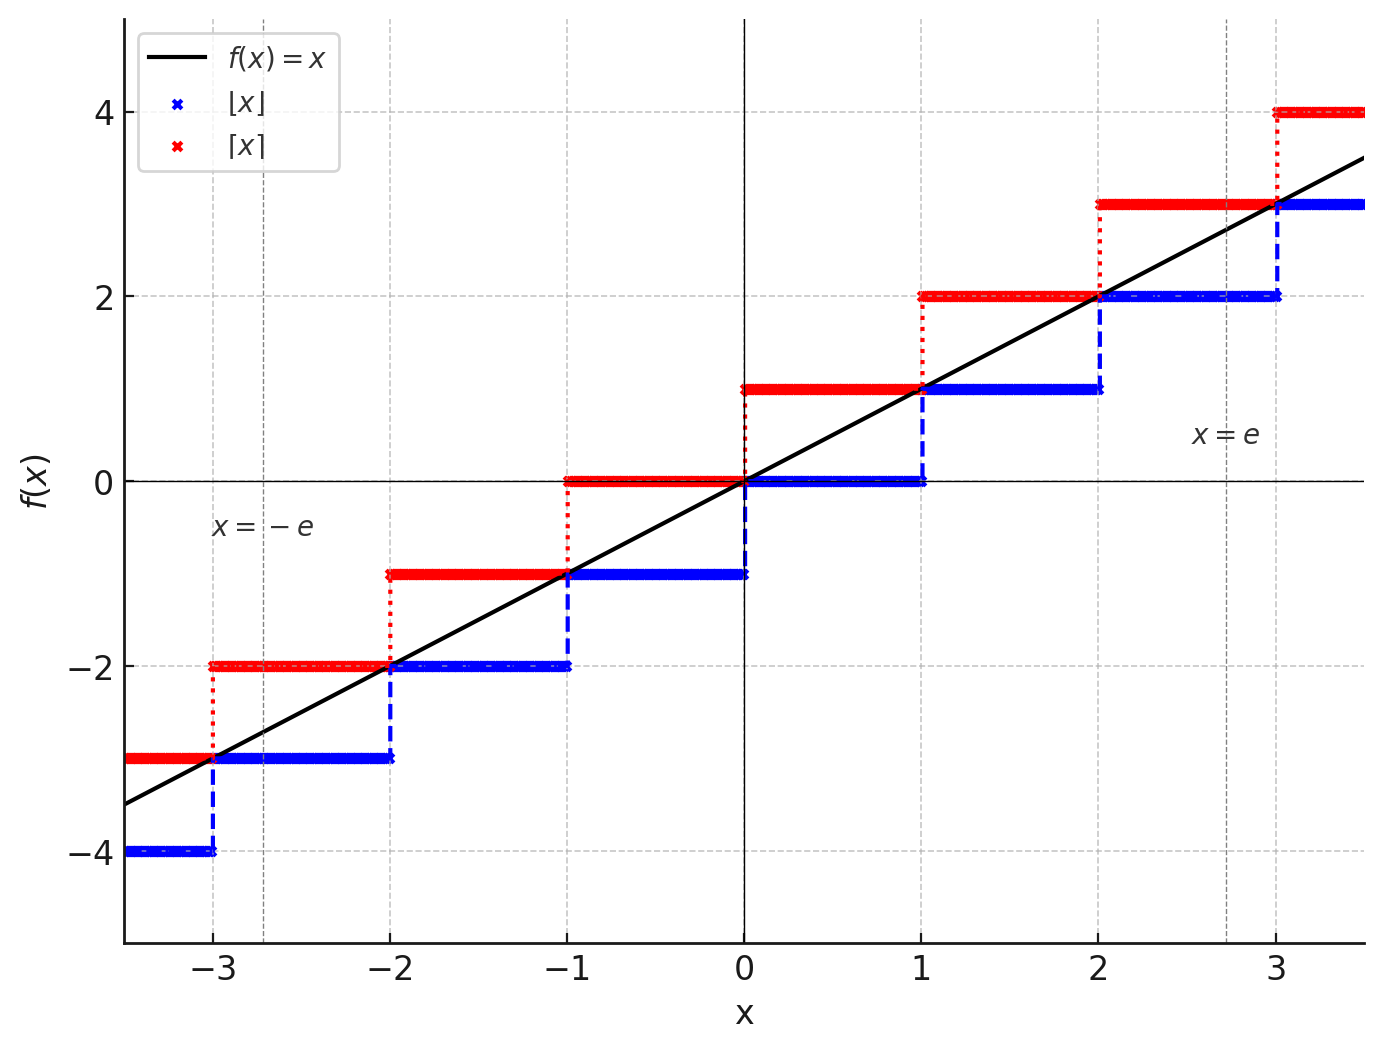
\includegraphics[width = 0.75\linewidth]{intfunc.png}
        \caption{Visualization of $\lceil x \rceil \text{ and } \lfloor x \rfloor$}
    \end{figure}

\begin{theorem}[Properties of Integer Function]
    Keep in mind the following important properties of integer function, which is 
    often used in algorithm analysis or other mathematical proof.
    \begin{enumerate}
        \item $\lfloor x \rfloor \leq x \leq \lceil x \rceil$
        \item  $\forall x\in \mathbb{Z} \text{, } \lceil x \rceil = \lfloor x \rfloor$
        \item $x \notin \mathbb{Z} \iff  \lceil x \rceil =  \lfloor x \rfloor+ 1  $
        \item $\lfloor -x \rfloor = -\lceil x \rceil $; $\lceil-x \rceil = - \lfloor x \rfloor$
        \item $x - 1 < \lfloor x \rfloor \leq x \leq \lceil x \rceil < x + 1$
    \end{enumerate}
\end{theorem}
The proofs to these conclusions are quite basic, and is therefore not provided here.

\subsubsection{Remainder and Integer Function}
We introduce a new operation that we have learned before in this section with its notation.
\begin{notation}[modulo operator]
    The modulo operation, denoted as \( a \bmod n \), finds the remainder when one integer \( a \) is divided by another integer \( n \). 
    If \( a \) divided by \( n \) gives a quotient \( q \) with remainder \( r \), then \( a = nq + r \), and \( r \) would be the result of \( a \bmod n \).
\end{notation}

Moving back to the integer function, we have:
\begin{theorem}
    $$\forall x, y \in \mathbb{R}, x \bmod y = x - y\left\lfloor \frac{x}{y} \right\rfloor, \quad \text{if } y \neq 0; \quad x \bmod 0 = x$$
\end{theorem}
Below is the proof to the first conclusion, where the properties of integer function are applied.
\begin{proof}
    By the Division Algorithm, for any integer \( x \) and any positive integer \( y \), there exist unique integers \( q \) and \( r \) such that \( x = qy + r \) and \( 0 \leq r < |y| \), where \( q \) is the quotient and \( r \) is the remainder. The floor function \( \left\lfloor \frac{x}{y} \right\rfloor \) yields the largest integer less than or equal to \( \frac{x}{y} \), which by definition is the quotient \( q \). Thus, we have:
\[
\left\lfloor \frac{x}{y} \right\rfloor = q
\]
and therefore:
\[
y\left\lfloor \frac{x}{y} \right\rfloor = yq
\]
Subtracting this from \( x \) gives:
\[
x - y\left\lfloor \frac{x}{y} \right\rfloor = x - yq = r
\]
The uniqueness of the quotient and remainder in the Division Algorithm ensures that this value of \( r \) is the remainder from the modulus operation. Therefore, we have:
\[
x \mod y = x - y\left\lfloor \frac{x}{y} \right\rfloor
\]
which is the remainder when \( x \) is divided by \( y \), completing the proof.

\end{proof}
Also, from definition, by dividing $y$ on both sides of the equation:
$$0\leq \frac{x}{y} - \lfloor\frac{x}{y}\rfloor = \frac{x \bmod y}{y} < 1$$
Among which, $x \bmod y <y$. 
\begin{proof}
    
        By the definition of the modulo operation, \( x \mod y \) can be written as \( x - y\left\lfloor \frac{x}{y} \right\rfloor \). Since \( \left\lfloor \frac{x}{y} \right\rfloor \) is the greatest integer less than or equal to \( \frac{x}{y} \), we have:
        \[
        x - y\left\lfloor \frac{x}{y} \right\rfloor \geq x - y \cdot \frac{x}{y} = x - x = 0.
        \]
        Furthermore, because \( \left \lfloor \frac{x}{y} \right\rfloor \) is less than \( \frac{x}{y} \), it follows that:
        \[
        x - y\left\lfloor \frac{x}{y} \right\rfloor < x - y \cdot \left(\frac{x}{y} - 1\right) = y.
        \]
        Hence, \( 0 \leq x \mod y < y \).

\end{proof}
And we have:
\begin{corollary}
    By above-mentioned conclusions:
    \begin{itemize}
        \item[a)] If $y > 0, \text{ then } 0 \leq x \bmod y < y$.
        \item[b)] If $y < 0, \text{ then}  0 \geq x \bmod y > y$.
        \item[c)]  $x - (x \bmod y) \text{ is an integral multiple of } y$.
    \end{itemize}
\end{corollary}
We call $x \bmod y$ the remainder when $x$ is divided by $y$. We call $\lfloor \frac{x}{y} \rfloor$ the quotient.
We have \( x \bmod y = 0 \) if and only if \( x \) is a multiple of \( y \), that is, if and only if \( x \) is divisible by \( y \). The notation \( y \mid x \), read ``\( y \) divides \( x \)'', means that \( y \) is a positive integer and \( x \bmod y = 0 \).
\subsection{exercises}
\begin{exercise}
    
        Let \( F \) be a field consisting of exactly three elements \( 0, 1, x \). Prove that \( x + x = 1 \) and that \( x \cdot x = 1 \). Obtain the addition and multiplication tables for \( F \).
        
\end{exercise}
    Hint: Think on the property of filed: inverse of addition and multiplication.
    \begin{proof}
        Since \( F \) is a field, it has the properties of both a group under addition and a group under multiplication (excluding \( 0 \) for the latter).
        
        \textbf{Part 1: Proof that \( x + x = 1 \)}
        \begin{enumerate}
            \item In a group, every element has an additive inverse. In \( F \), the additive inverse of \( 0 \) is \( 0 \) itself, since \( 0 + 0 = 0 \).
            \item The additive inverse of \( 1 \) cannot be \( 1 \) itself because \( 1 + 1 = 1 \) would imply \( 1 = 0 \), which is a contradiction. Therefore, \( 1 \)'s additive inverse must be some other element of \( F \), which can only be \( x \). Hence, \( 1 + x = 0 \).
            \item The element \( x \) must also have an additive inverse in \( F \), which cannot be \( 0 \) (as \( 0 \)'s inverse is \( 0 \)) and cannot be \( 1 \) (as \( 1 \)'s inverse is \( x \)). The only option left is \( x \) itself. Thus, \( x + x = 0 \).
            \item Given \( x + x = 0 \) and \( 1 + x = 0 \), by the cancellation law, it must be that \( x = 1 \). However, this contradicts the assumption that \( x \) is distinct from \( 1 \). Therefore, our assumption that \( x + x = 0 \) is incorrect.
            \item The only remaining possibility is \( x + x = 1 \).
        \end{enumerate}
        
        \textbf{Part 2: Proof that \( x \cdot x = 1 \)}
        \begin{enumerate}
            \item Similarly, in a multiplicative group (excluding \( 0 \)), every non-zero element has a multiplicative inverse. For \( 1 \), the multiplicative inverse is \( 1 \) itself since \( 1 \cdot 1 = 1 \).
            \item The element \( x \) must have a multiplicative inverse. It cannot be \( 0 \) since \( 0 \) is not invertible, and it cannot be \( 1 \) since \( 1 \) is already serving as its own inverse.
            \item The only remaining option for the multiplicative inverse of \( x \) is \( x \) itself. Hence, \( x \cdot x = 1 \).
        \end{enumerate}

        Now we construct the addition and multiplication tables for \( F \):

        \noindent
        \begin{minipage}{.5\textwidth}
        \centering
        \textbf{Addition Table:}
        \[
        \begin{array}{c|ccc}
        + & 0 & 1 & x \\
        \hline
        0 & 0 & 1 & x \\
        1 & 1 & x & 0 \\
        x & x & 0 & 1 \\
        \end{array}
        \]
        \end{minipage}%
        \begin{minipage}{.5\textwidth}
        \centering
        \textbf{Multiplication Table:}
        \[
        \begin{array}{c|ccc}
        \times & 0 & 1 & x \\
        \hline
        0 & 0 & 0 & 0 \\
        1 & 0 & 1 & x \\
        x & 0 & x & 1 \\
        \end{array}
        \]
        \end{minipage}
        \end{proof}
\begin{problem}
    Is there a field with exactly four elements? Is there a field with exactly six elements?
\end{problem}


\begin{exercise}
    Let \( n \) be an integer, and let \( x \) be a real number. Prove that:
\begin{enumerate}
    \item[a)] \( \lfloor x \rfloor < n \) if and only if \( x < n \);
    \item[b)] \( n \leq \lfloor x \rfloor \) if and only if \( n \leq x \);
    \item[c)] \( \lfloor x \rfloor \leq n \) if and only if \( x \leq n \);
    \item[d)] \( n < \lfloor x \rfloor \) if and only if \( n < x \);
    \item[e)] \( \lfloor x \rfloor = n \) if and only if \( x - 1 < n \leq x \) and if and only if \( n \leq x < n + 1 \);
    \item[f)] \( \lfloor x \rfloor = n \) if and only if \( x \leq n < x + 1 \) and if and only if \( n - 1 < x \leq n \).
\end{enumerate}
\end{exercise}
\begin{proof}
    \textbf{Part (a):} By definition, \( \lfloor x \rfloor \) is the greatest integer less than or equal to \( x \). Therefore, \( \lfloor x \rfloor < n \) means that \( x \) is less than \( n \) but not equal to it since \( \lfloor x \rfloor \) cannot be greater than \( x \).
    
    \textbf{Part (b):} If \( n \leq \lfloor x \rfloor \), then \( n \) must also be less than or equal to \( x \) because \( \lfloor x \rfloor \) is the greatest integer less than or equal to \( x \).
    
    \textbf{Part (c):} The statement \( \lfloor x \rfloor \leq n \) indicates that the largest integer less than or equal to \( x \) is also less than or equal to \( n \), which directly implies \( x \leq n \).
    
    \textbf{Part (d):} If \( n < \lfloor x \rfloor \), then \( n \) is strictly less than the integer part of \( x \), which means that \( n \) is also strictly less than \( x \).
    
    \textbf{Part (e):} For \( \lfloor x \rfloor = n \) to be true, \( x \) must be greater than \( n - 1 \) but not reach \( n + 1 \), hence the inequality \( x - 1 < n \leq x \) and \( n \leq x < n + 1 \).
    
    \textbf{Part (f):} Similarly, \( \lfloor x \rfloor = n \) if \( x \) has not reached \( n + 1 \) yet, which is the same as saying \( x \leq n < x + 1 \), and also if \( x \) is greater than \( n - 1 \) and less than or equal to \( n \), hence \( n - 1 < x \leq n \).
    \end{proof}

        \begin{exercise}
            Using the previous exercise, prove that \( \lfloor -x \rfloor = -\lceil x \rceil \).
            \end{exercise}
            
            \begin{proof}
                From the previous exercise, we have the following properties of the floor function for a real number \( x \) and an integer \( n \):
                \begin{enumerate}
                    \item \( x - 1 < \lfloor x \rfloor \leq x \);
                    \item \( n \leq x \) if and only if \( n \leq \lfloor x \rfloor \).
                \end{enumerate}
                Using these properties, we want to show that \( \lfloor -x \rfloor = -\lceil x \rceil \).
                
                Consider the number \( -x \). Applying property 1, we get:
                \[ -x - 1 < \lfloor -x \rfloor \leq -x \]
                Adding 1 to all parts of the inequality, we obtain:
                \[ -x < \lfloor -x \rfloor + 1 \leq -x + 1 \]
                Since \( \lceil x \rceil \) is the smallest integer greater than or equal to \( x \), \( \lfloor -x \rfloor + 1 \) is the smallest integer greater than \( -x \), which is \( -\lfloor x \rfloor \). Thus:
                \[ \lfloor -x \rfloor = -\lfloor x \rfloor - 1 = -\lceil x \rceil \]
                This completes the proof.
            \end{proof}
%------------------------------------------------------------






\section{Algorithm and Algorithm Analysis}
	This Section discusses what is algorithm, and more importantly, how algorithms
	are assessed.

    \subsection{Algorithm}
    \subsubsection{What is an Algorithm?}
    \begin{definition}[Algorithm] \label{def:algo}
        An algorithm is a well-defined, step-by-step procedure or sequence of instructions designed to solve a specific class of problems:
        \begin{itemize}
            \item Each step in an algorithm must be clear and unambiguous. 
            \item Algorithms must be solvable, meaning they should be able to produce a correct solution for any valid input within a finite amount of time.
            \item An algorithm must terminate, i.e., it should have a defined end, at which point the goal has been achieved and the final output is produced.
        \end{itemize} 
    \end{definition}
    Here is an example of multiplication algorithm for better understanding of the concept.
    \begin{example}[Russian Peasant Multiplication]
        To find the product of integers \( M \) and \( N \), both larger than one:

        \begin{enumerate}
            \item Start two columns on a page, one labeled ``A'' and the other ``B''; and put the value of \( M \) under A and the value of \( N \) under B.
            
            \item Repeat
            \begin{itemize}
                \item[(a)] calculate a new A-value by multiplying the old A-value by 2; and
                \item[(b)] calculate a new B-value by dividing the old B-value by 2 and reducing the result by a half if necessary to obtain an integer;
            \end{itemize}
            Until the B-value equals one.
            
            \item Go down the columns crossing out the A-value whenever the B-value is even.
            
            \item Add up the remaining A-values and ``return'' the sum.
        \end{enumerate}
    \end{example}
    To show how it works, assume $A=73$ and $B=41$.

\begin{table}[H]
\centering
\begin{tabular}{c|c}
\hline
A & B \\
\hline
73 & 41 \\
146 & 20 (20\(\frac{1}{2}\) is reduced to 20) \\
292 & 10 \\
584 & 5 \\
1168 & 2 (2\(\frac{1}{2}\) is reduced to 2) \\
2336 & 1 \\
\hline
\end{tabular}
\caption{Execution of RPM}
\end{table}

Sum of the remaining A-values: $2336+584+73=2993$.

Let's review this algorithm referring to definition \autoref{def:algo}. 
\begin{enumerate}
    \item Clarity and Accuracy: All the instructions are clear and manipulable, nothing is ambiguous.
    
    \item Solvability: It is no doubt that for any two real numbers, we can find their product.
    
    \item Termination: For which ever numbers, we can always solve the problem in limited steps, as the terminate condition is when $B=1$, while B is divided by 2 (integer division) repetitively. 
\end{enumerate}

Hence, the RPM is a good example of algorithm, and with this, we could tell whether
something else is an algorithm or not.
\subsubsection{Pseudocode}
Pseudocode is a simplified, half-code, half-natural language script used by software developers and algorithm designers to outline the structure of a program or algorithm. It's not executable code, but rather a high-level representation of the algorithm's logic. The purpose of pseudo-code is to express the design of an algorithm in a form that can be easily translated into actual programming languages. It is written in a way that is understandable to people who do not necessarily know the syntax of programming languages. Pseudo-code allows the designer to focus on the core logic of the algorithm without getting bogged down with the syntactic details of a particular programming language. It often uses control structures like if-then-else, while, for, and others that are common to many high-level languages.
Understanding pseudocode is quite easy as it quite close to natural languages.

Here's the RPM transcribed in pseudocode:
\begin{algorithm}[H]
	\caption{Russian Peasant Multiplication}\label{alg:rpm}
	\begin{algorithmic}[1]
	\Procedure{RPM}{$A, B$}
		\State $product \gets 0$
		\While{$B > 0$}
			\If{$B$ is odd}
				\State $product \gets product + A$
			\EndIf
			\State $A \gets A \times 2$
			\State $B \gets B \div 2$
		\EndWhile
		\State \textbf{return} $product$
	\EndProcedure
	\end{algorithmic}
	\end{algorithm}

    To explicit:
    \begin{itemize}
        \item \textbf{procedure RPM(A, B)}: Defines a procedure or function named `RPM` taking two parameters `A` and `B`.
        \item \textbf{product $\leftarrow$ 0}: The assignment operator `$\leftarrow$` is used to assign the value on the right (0 here) to the variable on the left (`product`).
        \item \textbf{while B $>$ 0 do}: Begins a `while` loop that continues as long as the condition `B $>$ 0` is true. The `do` indicates that the following block of code will execute if the condition is met.
        \item \textbf{if B is odd then}: A conditional statement that checks if `B` is odd. If it is, the subsequent statement is executed.
        \item \textbf{product $\leftarrow$ product + A}: An assignment operation that adds `A` to `product` and assigns the sum back to `product`.
        \item \textbf{end if}: Marks the end of the `if` statement.
        \item \textbf{A $\leftarrow$ A $\times$ 2}: Multiplies the value of `A` by 2 and then assigns the result back to `A`.
        \item \textbf{B $\leftarrow$ B $\div$ 2}: Divides the value of `B` by 2 (integer division) and assigns the result back to `B`.
        \item \textbf{end while}: Marks the end of the `while` loop.
        \item \textbf{return product}: The `return` statement indicates the output or result of the procedure, which here is the value of the variable `product`.
        \item \textbf{end procedure}: Marks the end of the `RPM` procedure.
    \end{itemize}
	All later algorithms in this book will be presented using pseudocode.
%------------------------------------------------

\subsection{Algorithm Analysis}

\par Now let's take a look at this algorithm from another aspects. Is this a good or a bad algorithm. People assess algorithms by examine its \textbf{complexity}, which could be either \textbf{space complexity} or \textbf{time complexity}. The former refers to the the relationship between the input and the space needed to execute the algorithm, the latter, similarly, refers to the time needed. Many tools are available to quantify complexity, for both space and time complexity, \textbf{the big O notation} is the most common measurement. 
\begin{definition}[The Big O Notation]\label{Big O}
    Big O notation is used to classify algorithms according to how their running time or space requirements grow as the input size grows. The notation describes an upper limit on the time an algorithm could possibly take to complete, given the size of the input. For a function \( f(n) \), where n is the scale of input for the algorithm, the Big O notation is formally defined as follows with $c$ as a positive constant:
    $$O(f(n)) = \{ g(n) : \text{Where } c \text{ and } n_0 
	\text{ such that } 0 \leq g(n) \leq c \cdot f(n) \text{ for all } n \geq n_0 \}$$
\end{definition}

The following table provides common time complexities using Big O notation:

\begin{table}[ht]
\centering
\begin{tabular}{@{}cc@{}}
\toprule
\( f(n) \) & Description \\ \midrule
1 & Constant \\
\( \log n \) & Logarithmic \\
n & Linear \\
\( n \log n \) & Linearithmic \\
\( n^2 \) & Quadratic \\
\( n^3 \) & Cubic \\
\( 2^n \) & Exponential \\ 
\(n!\) & Factorial \\
\bottomrule
\end{tabular}
\caption{Common time complexities in Big O notation}
\end{table}
We can visualize it using function graph
\begin{figure}[H]
    \centering
    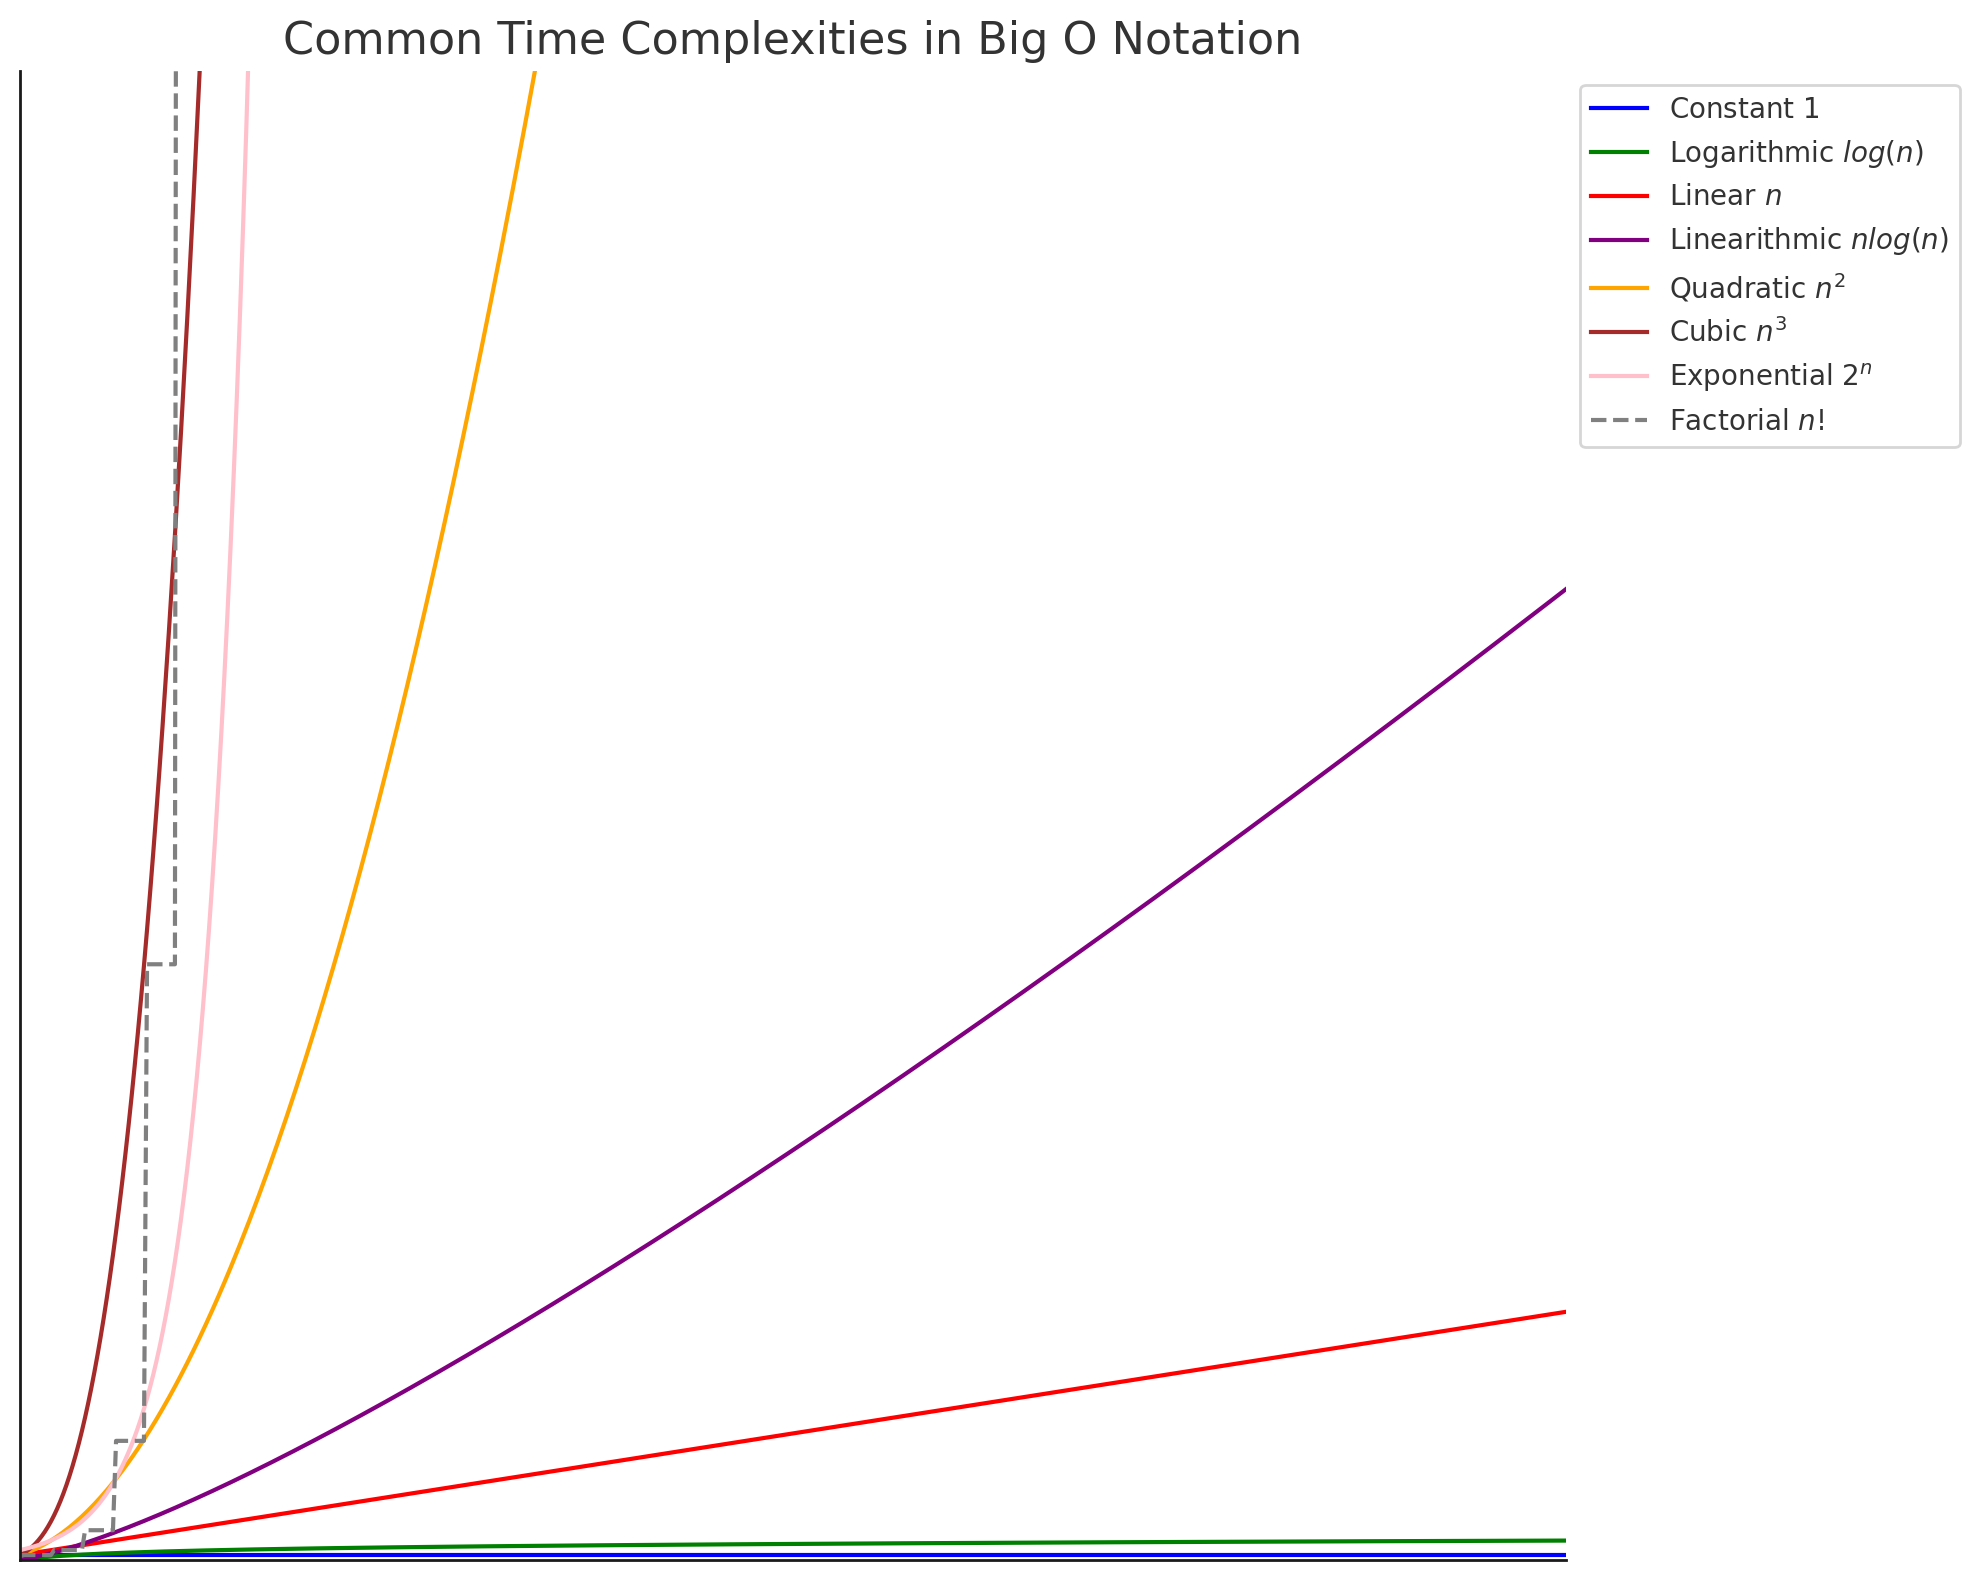
\includegraphics[width=0.8\linewidth]{Images/time complexity.png}
    \caption{Time Complexity Visualization}
    
\end{figure}
So which space and time complexity does this algorithm fall in? 
\subsubsection{Time Complexity}
To analyze the time complexity, we usually focus on the termination condition or the number of iteration for the algorithm. For the real number $B$ in RPM, each time it is divided by 2 until $B = 1$. Therefore, the total number of iteration will be $\log_2 B$, which is categorized in \( O(\log n) \).
\begin{remark}
    Actually, the time complexity of an algorithm could be shown by strict proof using MI. Here is the proof on the time complexity of RPM.
    \begin{proof}
        We will use mathematical induction to prove that the number of steps in the algorithm is proportional to \( \log_2(B) \).

\noindent \textbf{Base Case:}\\
When \( B = 1 \), the algorithm requires only one step. This is consistent with \( \log_2(1) = 0 \), which satisfies our complexity class \( O(\log n) \).

\noindent \textbf{Inductive Hypothesis:}\\
Assume that for a positive integer \( k \), when \( B = k \), the algorithm operates within \( \log_2(k) \) steps.

\noindent \textbf{Inductive Step:}\\
Consider \( B = 2k \). In the first step of the algorithm, \( B \) is halved to \( k \), and \( S \) is doubled. From this point, based on our inductive hypothesis, reaching \( B = 1 \) requires \( \log_2(k) \) steps.

Hence, for \( A = 2k \), the total number of steps is \( \log_2(k) + 1 \). Using the properties of logarithms, we have:
\begin{align*}
\log_2(k) + 1 &= \log_2(k) + \log_2(2) \\
&= \log_2(2k)
\end{align*}

Therefore, for any \( A = 2k \), the total number of steps is also \( \log_2(2k) \), proving that for any positive integer \( A \), the time complexity of the Russian Peasant Multiplication is \( O(\log A) \).
    \end{proof}
\end{remark}
%------------------------------------------------
\subsubsection{Space Complexity}
The space complexity of the Russian Peasant Multiplication algorithm is determined by the amount of memory required to store the operands and the intermediate results. Initially, only two numbers need to be stored: the multiplicands. As the algorithm proceeds, we need additional space to keep track of the current product. Since the algorithm does not use any complex data structures and only requires a fixed number of variables, the space complexity is \( O(1) \), indicating constant space usage. It does not depend on the size of the input operands, as the memory required does not increase with larger numbers.
%------------------------------------------------
\subsection{Exercises}
\begin{exercise}
    A non-recursive Square and Multiply Algorithm to calculate \( b^n \).

\textbf{Precondition:} \( n \) is a positive integer and \( b \) is of any type that can be multiplied.

\textbf{Postcondition:} the value returned is equal \( (b)^n \).

\begin{enumerate}
    \item Show that the algorithm terminates. Let \( a_k \) denote the value of \( a \) after the \( k \)th iteration of the while-loop, and let \( s = \lfloor \lg(n) \rfloor \). Prove by Mathematical Induction on \( k \) that For any nonnegative integer \( k \), after \( k \) iterations of the while-loop:
    $$2^{s-k} \le a_k < 2^{s-k+1}$$
    \item  Proof of correctness. Use Mathematical Induction on \( k \) to prove For any nonnegative integer \( k \), after \( k \) iterations of the while-loop:
\[ (\text{square})^a \times \text{product} = (b)^n \]
\end{enumerate}
\end{exercise}
\begin{algorithm}
    \caption{Square and Multiply Algorithm}
    \begin{algorithmic}[1]
    \State $product \gets 1$
    \State $square \gets b$
    \State $a \gets n$
    \While{$a > 1$}
        \If{$a \mod 2 \neq 0$} \Comment{If $a$ is odd}
            \State $product \gets product \times square$
        \EndIf
        \State $square \gets square \times square$
        \State $a \gets \lfloor a / 2 \rfloor$ \Comment{Integer division}
    \EndWhile
    \State \Return $product \times square$
    \end{algorithmic}
\end{algorithm}
\begin{proof}[1]
    \textit{Base Case} \(k=0\):
For \(k = 0\), \(a_0 = n\), which is the initial value of \(a\). Since \(s = \left\lfloor \lg(n) \right\rfloor\), it is the greatest integer less than or equal to \(\lg(n)\), therefore \(2^s \leq n < 2^{s+1}\). So, for \(k = 0\), the predicate holds because:
\[
\frac{2^s}{2^0} \leq a_0 = n < 2 \times \frac{2^s}{2^0}
\]

\textit{Inductive Step}:
Assume \(P(k)\) holds for some nonnegative integer \(k\). That is:
\[
\frac{2^s}{2^k} \leq a_k < 2 \times \frac{2^s}{2^k}
\]
We need to show \(P(k+1)\) holds. During each iteration, \(a\) is halved (integer division by 2), which gives us:
\[
a_{k+1} = \left\lfloor \frac{a_k}{2} \right\rfloor
\]

Since \(a_k\) is an integer, \(\left\lfloor \frac{a_k}{2} \right\rfloor\) will either be \(\frac{a_k}{2}\) or \(\frac{a_k - 1}{2}\), depending on whether \(a_k\) is even or odd. Thus, we have:
\[
\frac{2^s}{2^{k+1}} \leq \left\lfloor \frac{a_k}{2} \right\rfloor < 2 \times \frac{2^s}{2^{k+1}}
\]

Since \(a_k < 2 \times \frac{2^s}{2^k}\), dividing by 2 gives \(\frac{a_k}{2} < \frac{2^s}{2^k}\), and therefore:
\[
a_{k+1} < 2 \times \frac{2^s}{2^{k+1}}
\]

Similarly, \(\frac{2^s}{2^k} \leq a_k\) implies \(\frac{2^s}{2^{k+1}} \leq \frac{a_k}{2}\), so we have:
\[
\frac{2^s}{2^{k+1}} \leq a_{k+1}
\]
This completes the inductive step and thus, by induction, \(P(k)\) holds for all nonnegative integers \(k\).
\end{proof}
\begin{proof}[2]
    We need to prove that after \(k\) iterations of the while-loop, the invariant holds:
\[
(\text{square})^a \times \text{product} = b^n
\]

\textit{Base Case} \(k=0\):
Initially, \(\text{product} = 1\), \(\text{square} = b\), and \(a = n\). So,
\[
(\text{square})^a \times \text{product} = b^n
\]
is trivially true.

\textit{Inductive Step}:
Assume the invariant holds after \(k\) iterations, i.e.,
\[
(\text{square}_k)^{a_k} \times \text{product}_k = b^n
\]
Now, consider the \(k+1\)th iteration. There are two cases:

\textit{Case 1} (\(a_k\) is odd):
The product is updated by multiplying it with \(\text{square}_k\), and we have:
\[
\text{product}_{k+1} = \text{product}_k \times \text{square}_k
\]
Since \(a_k\) is odd, we can write \(a_k = 2m + 1\) for some integer \(m\), and after the iteration, \(a\) becomes \(a_{k+1} = m\). The invariant becomes:
\[
(\text{square}_k)^{2m+1} \times \text{product}_k = (\text{square}_k)^m \times \text{product}_{k+1} = b^n
\]

\textit{Case 2} (\(a_k\) is even):
The product remains the same, and \(a_k\) can be written as \(2m\), so the invariant remains:
\[
(\text{square}_k)^{2m} \times \text{product}_k = (\text{square}_k)^m \times \text{product}_k = b^n
\]
since \(\text{square}_{k+1} = (\text{square}_k)^2\) and \(a_{k+1} = m\).

In both cases, after the iteration, \(\text{square}\) is squared, so we get:
\[
\text{square}_{k+1} = (\text{square}_k)^2
\]
and therefore, the invariant still holds as:
\[
(\text{square}_{k+1})^{a_{k+1}} \times \text{product}_{k+1} = b^n
\]

Thus, by mathematical induction, the invariant holds true for every iteration of the loop, proving the correctness of the algorithm.
\end{proof}
%------------------------------------------------


%------------------------------------------------

\chapterimage{orange2.jpg}
\chapterspaceabove{6.75cm} 
\chapterspacebelow{7.25cm} 
\chapter{Inequality}
throughout our mathematical journey, equalities are always the very basics of most conclusion, and that is also which we start to learn math for. However, inequalities are not such a know thing as equalities.
Inequalities have many tricky characteristics so that we have to take with care, or things could go wrong. This chapter covers the fundamentals of inequality as a crucial tool for problem-solving in Computer Science.

\section{Inequality basics}
We all know about inequalities, and the first thing to clarify is the relationship between sizes. How to determine the size relationship between certain numbers? Since the basis for comparing "numbers" with each other corresponds to one, it is stipulated on the number line that the points increase from left to right, and therefore the numbers they represent increase in turn. Listed in ascending order, that is:

Let \( a, b \) be two real numbers, and the points on the number line are denoted as \( A, B \) respectively. If \( A \) is to the right of \( B \), we say \( a > b \); if \( A \) is to the left of \( B \), we say \( a < b \); if \( A \) coincides with \( B \), we say \( a = b \).

Thus, for any two real numbers, one and only one of the following three situations must hold:

\[
a > b; \quad a = b; \quad a < b.
\]

The above relationship is also known as the one-dimensional coordinate law.

\[
\begin{aligned}
a > b &\Leftrightarrow a - b > 0 \\
a < b &\Leftrightarrow a - b < 0 \\
a = b &\Leftrightarrow a - b = 0
\end{aligned}
\]

Where the symbol “\( \Leftrightarrow \)” (double arrow), read as "if and only if," means that the truth of two propositions depends on each other. That is to say, if one proposition is true, then the other proposition is also true; conversely, if one proposition is false, then the other proposition is also false.

Based on the derivation of inequalities, in most cases, the above principles are sufficient. The following mathematical laws involve the geometric and algebraic meanings of the sizes of real numbers and the relationship between them. They are the basis for comparing the sizes of two real numbers and for proving inequalities by comparison. Let's review some basic properties of inequalities that are the foundation for our further study.

\begin{itemize}
    \item Symmetry: \( a > b \) if and only if \( b < a \).
    \item Transitivity: If \( a > b \) and \( b > c \), then \( a > c \).
    \item Addition (Subtraction): If \( a > b \), then \( a + c > b + c \).
    \item Multiplication (Division): If \( a > b \) and \( c > 0 \), then \( ac > bc \); if \( a > b \) and \( c < 0 \), then \( ac < bc \).
    \item Exponentiation: If \( a > b \), then \( a^n > b^n \), where \( n \) is a positive integer, and \( n \geq 2 \).
    \item Root Extraction (Power Root): If \( a > b > 0 \), then \( \sqrt[n]{a} > \sqrt[n]{b} \), where \( n \) is a positive integer, and \( n \geq 2 \).
    \item If \( a > b \) and \( c > d \), then \( a + c > b + d \).
    \item If \( a > b > 0 \) and \( c > d > 0 \), then \( ac > bd \).
\end{itemize}
\subsection{Exercises}
\begin{exercise}
    Explain the following statement.
    \begin{enumerate}
        \item If \( a > b \), then \( \frac{a}{c} > \frac{b}{c} \);
        \item If \( ac < bc \), then \( a < b \);
        \item If \( a < b \), then \( \frac{1}{a} > \frac{1}{b} \);
        \item If \( ac^2 > bc^2 \), then \( a > b \);
        \item If \( a > b \), then \( a^n > b^n \).
    \end{enumerate}
\end{exercise}

\textbf{Solution:}

\begin{enumerate}
    \item If \( c > 0 \), multiplying both sides of \( a > b \) by the positive number \( \frac{1}{c} \) preserves the inequality, hence \( \frac{a}{c} > \frac{b}{c} \). If \( c < 0 \), the direction of the inequality would be reversed, which is not given in the condition, hence we assume \( c > 0 \).
    \item Dividing both sides of \( ac < bc \) by \( c \) (assuming \( c \neq 0 \)), we get \( a < b \) because division by a positive number preserves the inequality, and division by a negative number reverses it.
    \item Taking the reciprocal of both sides of \( a < b \) reverses the inequality because \( a \) and \( b \) are on opposite sides of the fraction line, hence \( \frac{1}{a} > \frac{1}{b} \) (assuming \( a, b > 0 \) to avoid division by zero).
    \item Dividing both sides of \( ac^2 > bc^2 \) by \( c^2 \) (assuming \( c \neq 0 \)) preserves the inequality, hence \( a > b \) because \( c^2 \) is positive regardless of whether \( c \) is positive or negative.
    \item Raising both sides of \( a > b \) to a power \( n \) (assuming \( n \) is a positive integer) preserves the inequality because both \( a \) and \( b \) are raised to the same power, hence \( a^n > b^n \).
\end{enumerate}
\begin{exercise}
    Given the inequality \( a > b > 0 \), \( c < d < 0 \), \( f < 0 \), show that:
\[
\frac{f}{a - c} > \frac{f}{b - d}.
\]
\end{exercise}
\begin{proof}
    Since \( a > b > 0 \) and \( c < d < 0 \), then \( a - c > b - d \) because subtracting a smaller negative number is the same as adding a larger positive number. Given that \( f < 0 \), when dividing by a larger positive number, the result is smaller because a negative number divided by a positive number yields a negative result, and the further away the divisor is from zero, the smaller the quotient.

Therefore:
\[
\frac{f}{a - c} > \frac{f}{b - d}.
\]
\end{proof}

\section{Solving Quadratic Inequality}
Recall that, when we solve Quadratic equations, we use discriminant to solve equations, which is also applicable to inequalities.
For a quadratic inequality of the form $ax^2 + bx + c > 0$ or $ax^2 + bx + c < 0$ (where $a > 0$), the solution set can be determined by the discriminant $\Delta = b^2 - 4ac$:
\begin{enumerate}
    \item If $\Delta > 0$, the quadratic equation $ax^2 + bx + c = 0$ has two distinct real roots $x_1$ and $x_2$, and $x_1 < x_2$. The solution set for $y = ax^2 + bx + c$ being greater than zero (when $y = 0$) is for values of $x$ either less than $x_1$ or greater than $x_2$, and the solution set for $ax^2 + bx + c < 0$ is $\{ x \mid x_1 < x < x_2 \}$.
    \item If $\Delta = 0$, then $ax^2 + bx + c = 0$ has one real root, specifically $x_1 = x_2 = -\frac{b}{2a}$. The solution set for $y = ax^2 + bx + c$ being greater than zero is all $x$ except $x \neq -\frac{b}{2a}$, and there is no solution set where $ax^2 + bx + c < 0$.
    \item If $\Delta < 0$, then $ax^2 + bx + c = 0$ has no real roots, and the parabola $y = ax^2 + bx + c$ does not intersect the x-axis. The solution set for $ax^2 + bx + c > 0$ is all real numbers, and there is no solution set where $ax^2 + bx + c < 0$.
\end{enumerate}
\begin{figure}[ht!]
    \centering
    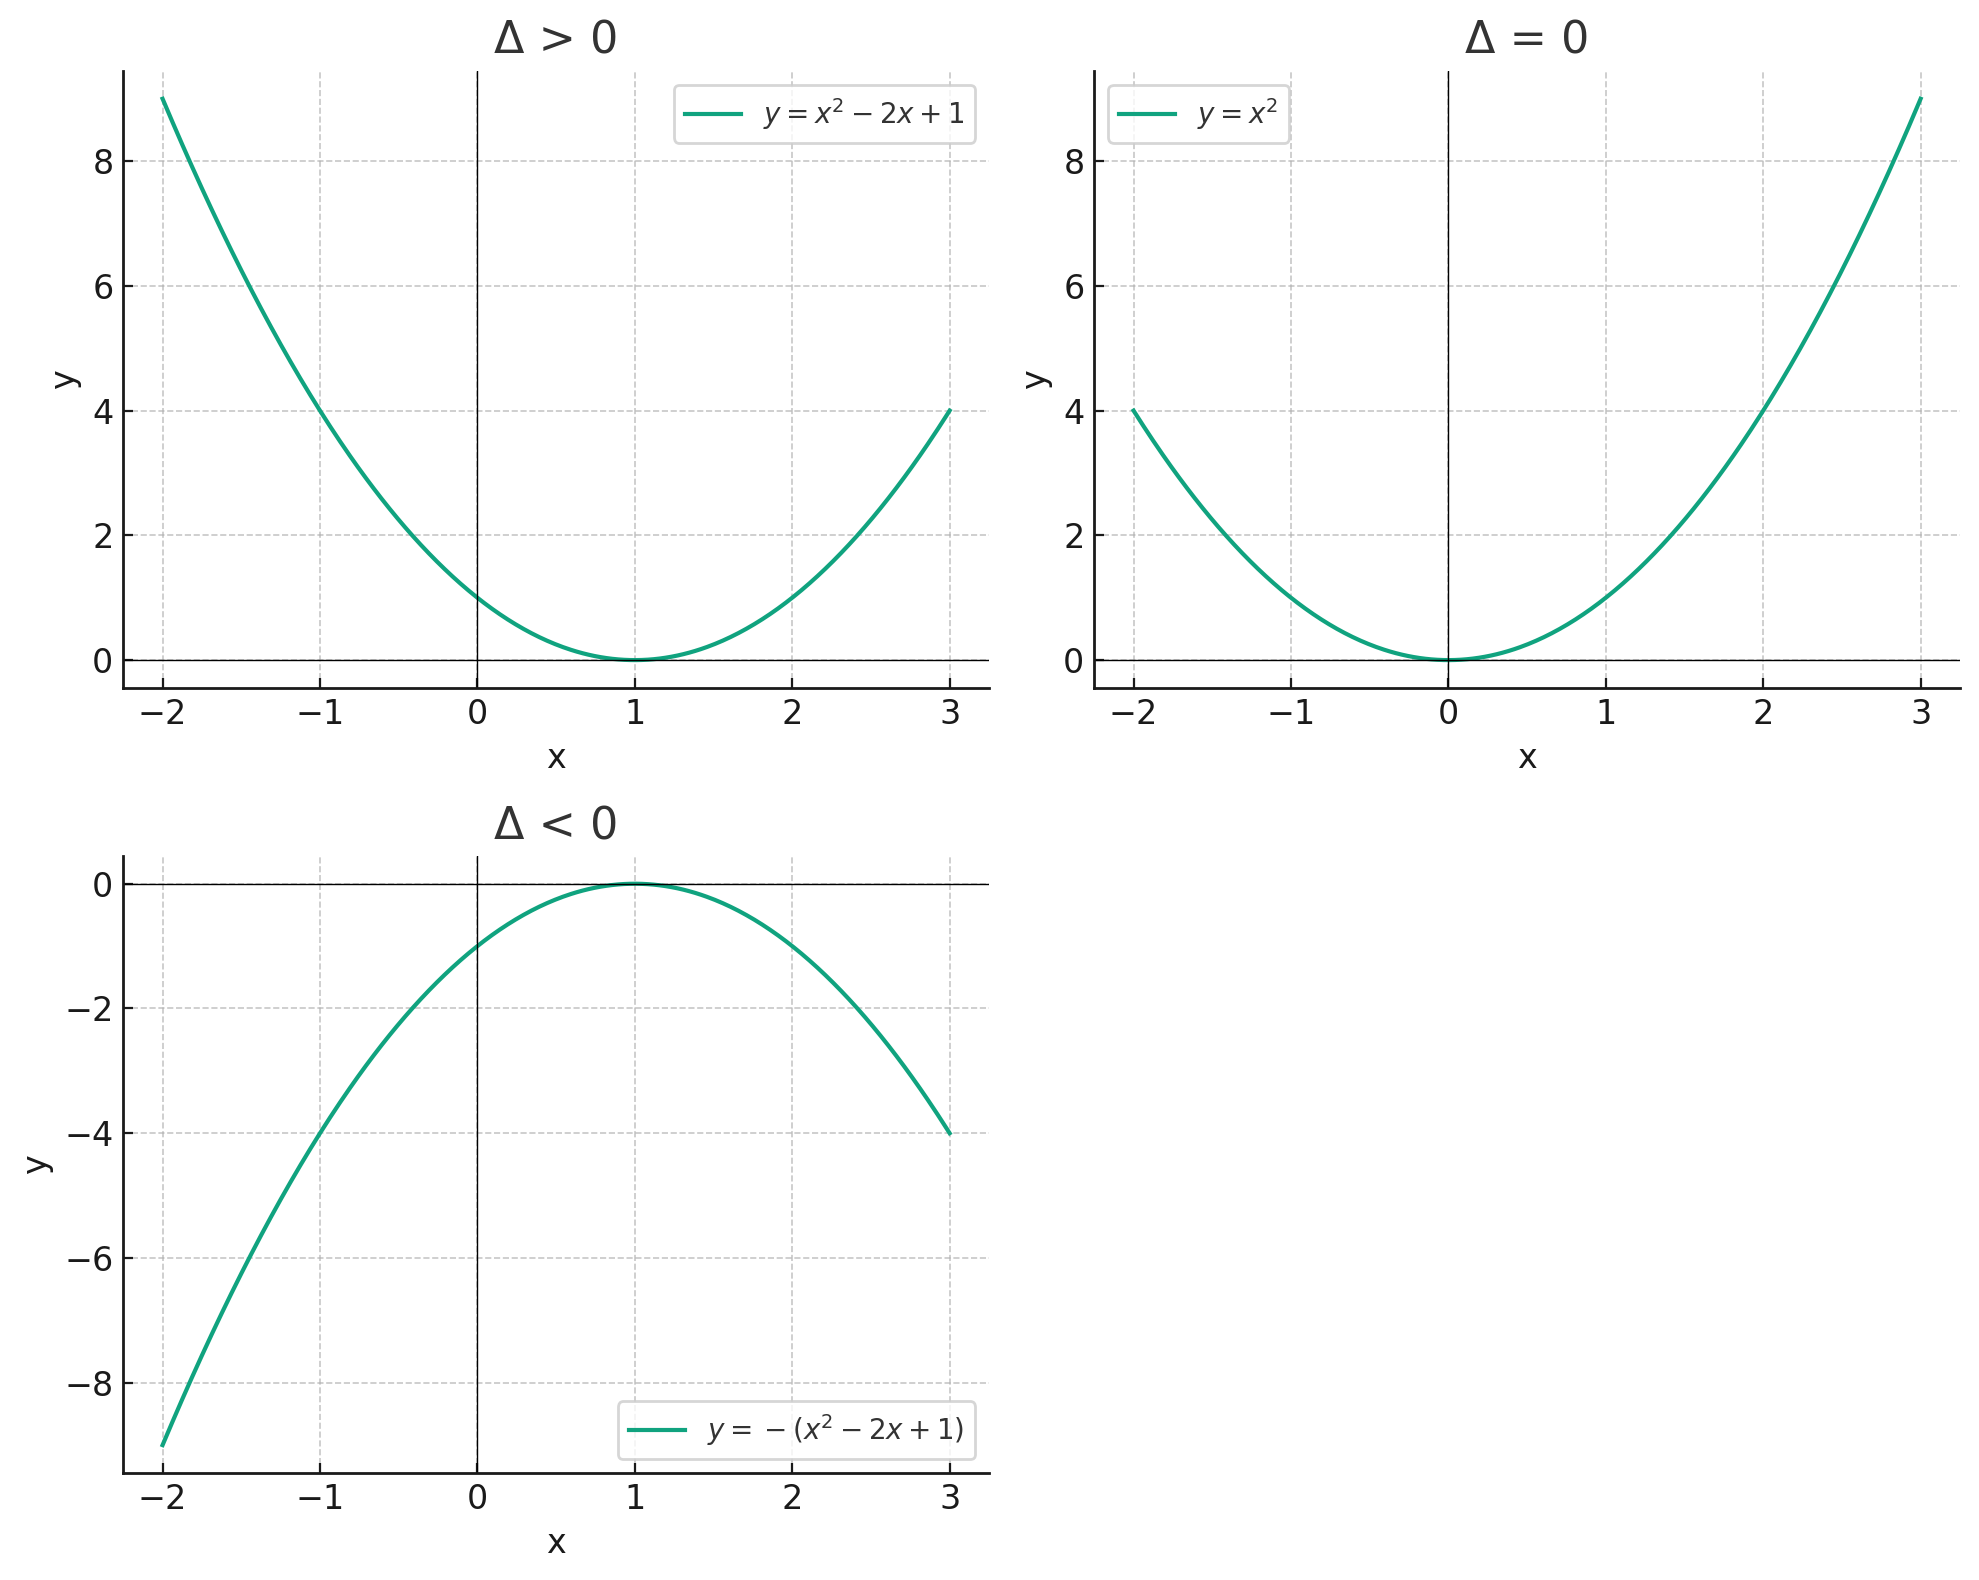
\includegraphics[width=0.8\textwidth]{quadratic.png}
    \caption{Quadratic function graphs based on the discriminant.}
\end{figure}
\begin{example}
    Solve the following quadratic inequalities:

\begin{enumerate}
    \item \(4x^2 + 6x + 2 < 0\);
    \item \(4x^2 + 4x + 1 < 0\);
    \item \(-3x^2 + x - 6 < 0\).
\end{enumerate}
\end{example}
\textbf{Solution:}

\begin{enumerate}
    \item The discriminant \(\Delta = 6^2 - 4 \times 4 \times 2 = 4 > 0\), so the quadratic equation \(4x^2 + 6x + 2 = 0\) has two real roots \(x_1 = -1\), \(x_2 = -\frac{1}{2}\).
    Hence, the solution set for the inequality is \(x \in \left(-\infty, -1\right) \cup \left(-\frac{1}{2}, \infty\right)\).

    \item The discriminant \(\Delta = 4^2 - 4 \times 4 \times 1 = 0\), so the quadratic equation \(4x^2 + 4x + 1 = 0\) has one real double root. Therefore, the inequality has no solution set.

    \item The discriminant \(\Delta = 1^2 - 4 \times (-3) \times (-6) = -71 < 0\), so the quadratic equation \(-3x^2 + x - 6 = 0\) has no real roots.
    Therefore, the solution set for the inequality \(3x^2 - x + 6 > 0\) is all real numbers, and thus the solution set for the given inequality is also all real numbers.
\end{enumerate}

\section{important Inequalities}
In this part, we explore two fundamental inequalities in mathematics: the Triangle Inequality and the Arithmetic-Geometric Mean (AGM) Inequality. Each section provides a comprehensive overview, including detailed proofs and corollaries.
\subsection{The Triangle Inequality}
The Triangle Inequality is a fundamental relation in geometry and analysis, asserting that the sum of the lengths of any two sides of a triangle must be greater than or equal to the length of the remaining side.
    \begin{definition}[Triangular Inequality] \label{triangularineq}
        For any real numbers \( a \) and \( b \), the Triangle Inequality is given by:
        \[ |a + b| \leq |a| + |b| \]
    \end{definition}
    \begin{proof}
        The proof of the Triangle Inequality considers the sign of \( a \) and \( b \):
    \begin{itemize}
     \item \textbf{Case 1:} If \( a \) and \( b \) have the same sign, the inequality follows directly.
        \item \textbf{Case 2:} If \( a \) and \( b \) have opposite signs, assume \( a > 0 \) and \( b < 0      \). Then, \( |a + b| \leq a - b = |a| + |b| \).
    \end{itemize}
    Thus, the Triangle Inequality is proven.
    \end{proof}
    \begin{remark}
        This important inequality will also be seen in other chapters.
    \end{remark}
We also have the following conclusion by preliminary algebra:
$$
\begin{aligned}
    |a{+}b|{\leqslant}|a|+|b|& \Leftrightarrow|a{+}b|^2{\leqslant}(|a|{+}|b|)^2  \\
    &\Leftrightarrow(a+b)^2\leqslant|a|^2+2|a||b|+|b|^2 \\
    &\Leftrightarrow a^2+2ab+b^2\leqslant a^2+2|a|\mid b|+b^2 \\
    &\Leftrightarrow ab{\leqslant}|a|\left|b\right| \\
    &\Leftrightarrow ab\leqslant\lvert ab\rvert.
    \end{aligned}
$$
The quality holds only when $ab \geq 0$.
\subsubsection*{Geometric Explanation of Triangular Inequality}
    Consider $a$ and $b$ are random numbers on a number axis:
    \begin{itemize}
        \item If $ab \geq 0$, then they are both in the same half-axis (both positive or negative). In this case, the distance between $a$ and $-b$
        is the sum of the distance from both points to the origin of the number axis.
        \item  Now consider $ab < 0$, either of them is positive, and the other is negative. In this case, the distance between $a$ and $-b$ is shorter than the sum of 
        the distance from both points to the origin of the number axis.
        \begin{figure}[H]
            \centering
            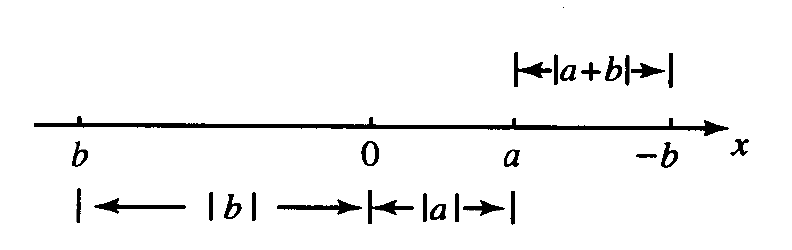
\includegraphics[width = 0.6\textwidth]{triangleablt0.png}
            \caption{Triangular Inequality: $ab < 0$}
        \end{figure}
    \end{itemize}

We also have:
    \begin{theorem}
        For $a, b, c\in \mathbb{R}$, $|a-c|\leq |a-b| + |b-c|$.
    \end{theorem}
    \begin{figure}[H]
        \centering
        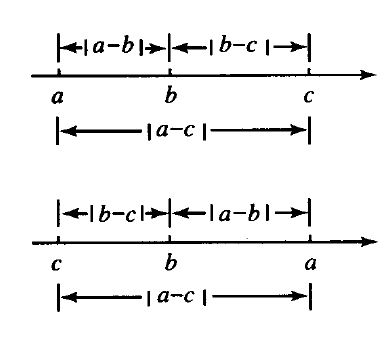
\includegraphics[width = 0.5\textwidth]{triangle2.png}
    \end{figure}
    \begin{proof}
        Since $a-c$, $a-b$, $b-c$ follows the relationship of triangular inequality. We have:
        $$(a-b)(b-c) \geq 0$$
        
        meaning that $b$ is between $a$ and $c$, which could be proven by sketching.
    \end{proof}

    \begin{corollary} \label{trian}
        $||a| - |b|| \leq |a + b|$
    \end{corollary}
    \begin{proof}
        \[ |a| = |(a+b) - b| \leq |a+b| + |-b| = |a+b| + |b|. \]
Therefore,
\[ |a| - |b| \leq |a+b|, \]
and similarly it can be proven that
\[ |b| - |a| \leq |a+b|. \]
Hence,
\[ ||a - b|| \leq |a+b|. \]
    \end{proof}

    \begin{corollary}
        $|a| - |b| \leq |a + b|$
        
    \end{corollary}
    \begin{proof}
        By corollary \autoref{trian}:
        \[ ||a| - |b|| \leq |a + (-b)|, \]
therefore,
\[ ||a| - |-b|| \leq |a - b|. \]
    \end{proof}
%---------------------------------------------------------------------------
    \subsection{The Arithmetic-Geometric Mean Inequality}
    The AGM Inequality(also known as AM-GM inequality) states that for any set of non-negative real numbers, the arithmetic mean is always greater than or equal to the geometric mean.
    \begin{definition}[AGM Inequality] \label{AGM}
        For non-negative real numbers \( a_1, a_2, \ldots, a_n \), the AGM Inequality is:
        \[ \frac{a_1 + a_2 + \cdots + a_n}{n} \geq \sqrt[n]{a_1 \cdot a_2 \cdots a_n} \]
    \end{definition}
    Many methods are available to prove this important conclusion. Below is the proof by MI.
    \begin{proof}
        We prove that for any non-negative real numbers \(x_1, \ldots, x_n\), the following inequality holds:

\[
\alpha^n \geq x_1 x_2 \cdots x_n
\]

where \( \alpha \) is the arithmetic mean of the numbers, with equality if and only if all the numbers are equal.
\begin{remark}
    This is because, the inequality is equivalent to AGM:
    $$\frac{a_{1} +a_{2} +\dotsc +a_{n}}{n} \geq \sqrt[n]{a_{1} \cdot a_{2} \dotsc a_{n}} \Longleftrightarrow \left(\frac{a_{1} +a_{2} +\dotsc +a_{n}}{n}\right)^{n} \geq a_{1} \cdot a_{2} \dotsc a_{n}$$

\end{remark}
\textbf{Induction Basis:}
For \(n = 1\), the statement is trivially true, as the arithmetic mean of a single number is the number itself.

\noindent \textbf{Induction Hypothesis:}
Assume that the AM-GM inequality holds for \(n\) non-negative real numbers.

\noindent \textbf{Induction Step:}
Consider \(n+1\) non-negative real numbers \(x_1, \ldots, x_{n+1}\). Their arithmetic mean \( \alpha \) satisfies:

\[
\alpha = \frac{x_1 + \cdots + x_n + x_{n+1}}{n+1}
\]

If all the \(x_i\) are equal to \( \alpha \), then we have equality in the AM-GM statement, and we are done. In the case where some are not equal to \( \alpha \), there must exist at least one number greater and one smaller than \( \alpha \). Without loss of generality, we can reorder our \(x_i\) to ensure that \(x_n > \alpha > x_{n+1}\), which gives us:
\begin{equation}
    (x_n - \alpha)(\alpha - x_{n+1}) > 0 \label{agm1}
\end{equation}


Define a new number \( y \) with:

\[
y = x_n + x_{n+1} - \alpha \geq x_n - \alpha > 0
\]
Since all numbers from $x_1$ to $y$  are non-negative.

$$\begin{aligned}&(n+1)\alpha=x_1+\cdots+x_{n-1}+x_n+x_{n+1}\\&n\alpha=x_1+\cdots+x_{n-1}+\underbrace{x_n+x_{n+1}-\alpha}_{=y},\end{aligned}$$

This shows that $\alpha$ is also a geometric mean of the n-sequence $x_{1},\ldots,x_{n-1},y$. 

By the induction hypothesis:
$$\alpha^{n+1}=\alpha^n\cdot\alpha\geq x_1x_2\cdots x_{n-1}y\cdot\alpha.$$

From equation \autoref{agm1}, we have:
$$(\underbrace{x_n+x_{n+1}-\alpha}_{=y})\alpha-x_nx_{n+1}=(x_n-\alpha)(\alpha-x_{n+1})>0,$$

Hence:
$$y\cdot \alpha > x_n x_{n+1}$$
By substituting we have:
$$\alpha^{n+1}>x_1x_2\cdots x_{n-1}x_nx_{n+1}$$
This completes the proof.
\end{proof}

\subsubsection*{Geometric representation}
We can use function graphs to visualize the relationship implied in the AGM inequality. On the left and right-hand-side of the inequality sign, there are two functions with $n$ variables.
For simplicity, we use $n=2$ to show its visualization.
We obtain this interactive graph by Mathematica. This simple model involves three variables only. $\displaystyle x_{1}$ and $\displaystyle x_{2}$ are the values to be used to calculate AM and GM. 
We take one of the input value as preimage on the x-axis, and the AM or GM as the image on y-axis. The scroll on the top indicates the value of $\displaystyle x_{2}$. When $\displaystyle x_{2} =0$, the 
graph is shown below. It can be seen that the AGM inequality holds, and only when $\displaystyle x_{2} =x_{1} =0$, there is an intersection$\displaystyle \ ( 0,0) .$

\begin{figure}[H]
    \centering
    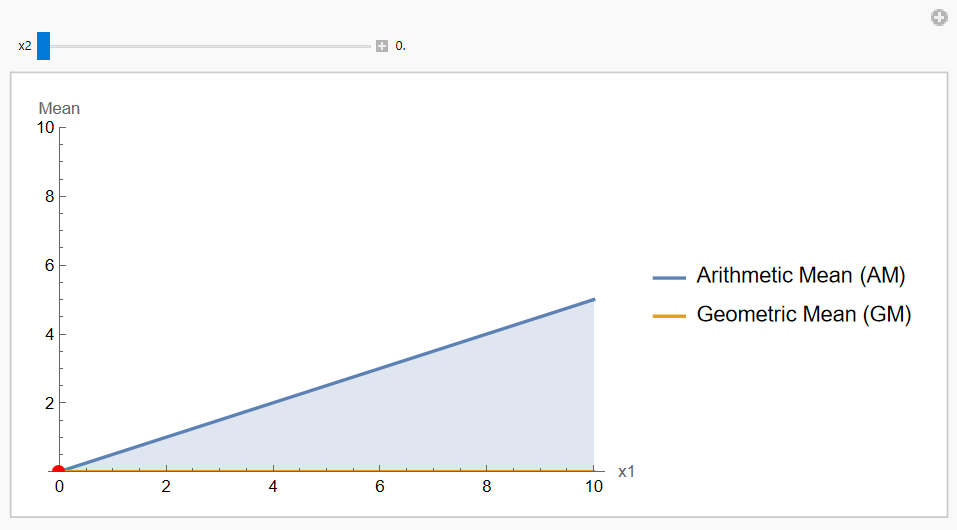
\includegraphics[width=0.8\textwidth]{agmx=0.png}
    \caption{AGM when $x_2 = 0$}
\end{figure}

As we increase the $\displaystyle x_{2}$ value, the GM curve rise up, and the intersection moves on the right direction, remaining on the AM curve. Below is the visualization for $\displaystyle x_{2} =5$. 
There is no any overlap between graphs except the intersection $\displaystyle ( 5,5)$. 

\begin{figure}[H]
    \centering
    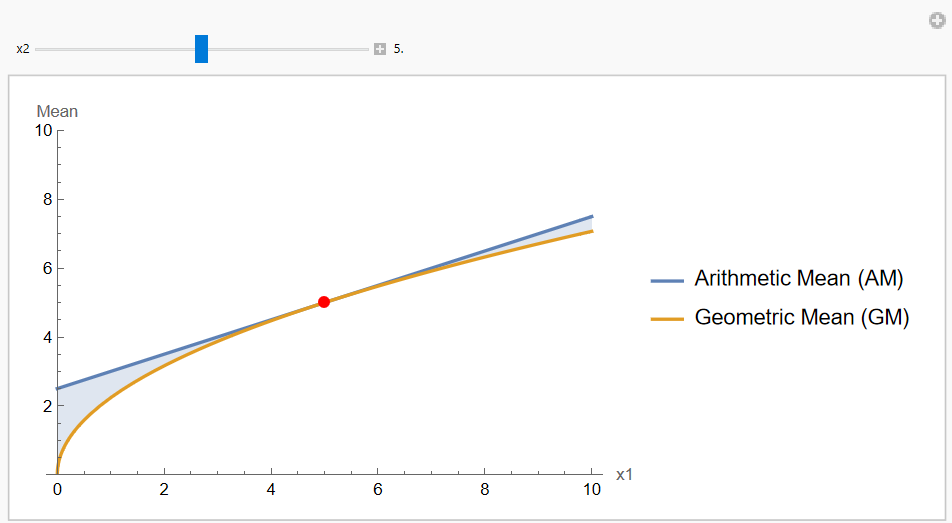
\includegraphics[width=0.8\textwidth]{agmx=5.png}
    \caption{AGM when $x_2 = 5$}
\end{figure}

\begin{problem}
    Where will the intersection go if we have $x_2 = 10$ for this model?
\end{problem}

Now, I think everything is clear, but only things so far. From now on, we will extend the understanding of function graph to a new
dimension, in the 3 dimension space. Functions in the 3D space is extremely important for multi-variable calculus, and learning linear 
algebra also requires us to abstract numbers in more than 3 dimension, but goes up to n dimension space. But don't worry, the discussion
here only involve simple concepts. 

We have three variables: $x_1, x_2, y$, where $y$ is the value of AM or GM from $x_1$ and $x_2$. Coincidently, we have three coordinate
axis in a 3D space. In the three-dimensional coordinate system, we assign two preimages $x_1$, $x_2$ to $x$ and $y$ axis, and the mean
to the $z$ axis. In this way we can get two function graphs, or surface, in the real sense, in the coordinate, which look like in the 
figure below.
\begin{figure}[H]
    \centering
    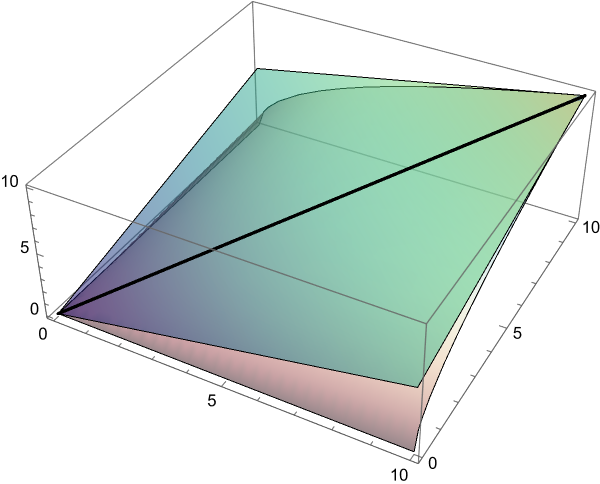
\includegraphics[width=0.6\textwidth]{agm3D.png}
    \caption{AGM 3D Visualization}
\end{figure}

The plane in blue represents the set of all possible arithmetic mean derived from all combinations of $x_1 \text{ and }x_2$ with $x_1,x_2\in [0,10]$, and the other 
surface, almost below the AM plane, is exactly the geometric mean curve that has a similar definition to the former. This is quite different from the functions
we have known, since they are only a line or a curve in the Cartesian coordinate, yet in the 3D coordinate, function could be surface. We will explore more
about multi-variable functions in the future. 

It is noticeable that the two surfaces are actually independent. They intersect in a line that go across the space. That specific line is actually a set of all the
ordered pairs $(x_1,x_2)$ where $x_1 = x_2$. We can actually relate it to the graph in the Cartesian coordinate. If we change the view point to the front of the
curves shaped in the 3D space, we see something like this picture.
\begin{figure}[H]
    \centering
    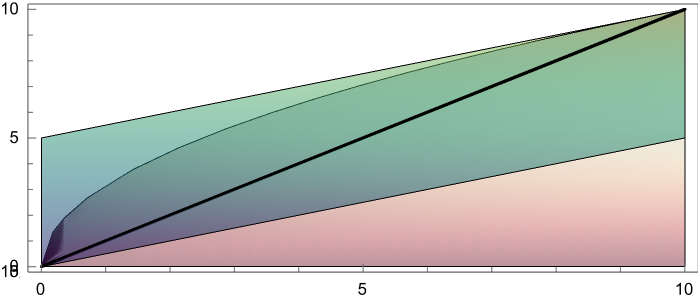
\includegraphics[width=0.6\textwidth]{agm3dsect.png}
    \caption{AGM 3D Visualization (Front)}
\end{figure}
Isn't this quite similar to the 2D graph? Actually, the first image is exactly a horizontal cross-section of the 3D function graph, and the intersection in the 2D 
graph changes as the position of intersection line changes. These explain AGM inequality's geometric meaning.

\subsection*{Conclusions of AGM inequality}
AGM inequality has brought us to these conclusions:
    \begin{corollary}[Mean Inequality Corollary]
If $x, y > 0$, then
\[\frac{2xy}{x+y} \leq \sqrt{xy} \leq \frac{x+y}{2}.\]
Equality holds in each inequality only when $x = y$.
\end{corollary}

\begin{proof}
Proposition \ref{AGM} yields $\sqrt{xy} \leq \frac{x+y}{2}$. We obtain the other inequality from this by multiplying both sides by the positive number $\frac{2\sqrt{xy}}{x+y}$, leading to:
\[\sqrt{xy} \cdot \frac{2\sqrt{xy}}{x+y} \leq \frac{x+y}{2} \cdot \frac{2\sqrt{xy}}{x+y},\]
which simplifies to:
\[\frac{2xy}{x+y} \leq \sqrt{xy}.\]
Thus, we have shown that $\frac{2xy}{x+y} \leq \sqrt{xy} \leq \frac{x+y}{2}$, with equality if and only if $x = y$.
\end{proof}
The expression $\frac{2xy}{x+y}$ is the harmonic mean of $x$ and $y$. It arises in the study of average rates. For example, consider traveling a distance $d$ at rate $r_1$ in time $t_1$ and making the return trip at rate $r_2$ in time $t_2$. The harmonic mean gives us the average rate $r$ for the full trip.

Assuming we travel the same distance $d$ for both trips, we have:
\begin{align*}
r_1t_1 &= d \\
r_2t_2 &= d
\end{align*}

The average rate $r$ for the full trip is computed as follows:
\begin{align*}
r &= \frac{2d}{t_1 + t_2} = \frac{2d}{\frac{d}{r_1} + \frac{d}{r_2}} = \frac{2d}{\frac{r_1r_2(t_1 + t_2)}{r_1r_2}} =\frac{2r_1r_2}{r_1 + r_2}\\
\end{align*}

The other important corollary of AGM inequality is:
\begin{corollary}
    $a^2+b^2 \geq 2ab$
\end{corollary}
\begin{proof}
    $a^2 + b^2 \geq 2ab \iff a^2 + b^2 - 2ab \geq 0 \iff (a - b)^2 \geq 0.$
\end{proof}


\subsection{Exercises}
\begin{exercise}
    Prove that for any triangle with sides \(a\), \(b\), and \(c\), the following inequality holds:
\[ \frac{a}{b + c} + \frac{b}{a + c} + \frac{c}{a + b} > 1 \]
\end{exercise}
\begin{proof}

Given a triangle with sides \(a\), \(b\), and \(c\), we know that for any triangle, the sum of the lengths of any two sides is greater than the length of the third side. Therefore, \(a < b + c\), \(b < a + c\), and \(c < a + b\).

Now, consider the inequality \(\frac{a}{b + c} > \frac{a}{a + b + c}\). This is true because \(b + c > a\) implies that the denominator of the left-hand side is smaller than that of the right-hand side while keeping the numerator constant.

Similarly, we can show that \(\frac{b}{a + c} > \frac{b}{a + b + c}\) and \(\frac{c}{a + b} > \frac{c}{a + b + c}\).

Adding these three inequalities, we get:
\[ \frac{a}{b + c} + \frac{b}{a + c} + \frac{c}{a + b} > \frac{a + b + c}{a + b + c} \]

Simplifying the right-hand side, we obtain:
\[ \frac{a}{b + c} + \frac{b}{a + c} + \frac{c}{a + b} > 1 \]

Thus, the inequality is proven. 

\end{proof}

\begin{exercise}
    Given $\varepsilon > 0$, if $|x - a| < \frac{\varepsilon}{4}$ and $|y - b| < \frac{\varepsilon}{6}$, prove that:

\[
|2x + 3y - 2a - 3b| < \varepsilon.
\]
\end{exercise}
Hint: Rearrange it in a form that is good for using triangle inequality.
\begin{proof}
    \begin{align*}
        |2x + 3y - 2a - 3b| &= |2(x - a) + 3(y - b)| \\
        &\leq |2(x - a)| + |3(y - b)| \\
        &= 2|x - a| + 3|y - b| \\
        &< 2 \times \frac{\varepsilon}{4} + 3 \times \frac{\varepsilon}{6} \\
        &= \varepsilon.
        \end{align*}
\end{proof}

\begin{exercise}
    Prove for any real numbers \( a, b, c, d \) that:
\[ |a - b| + |b - c| + |c - d| + |d - a| \geq |a - c| + |b - d| \]

\end{exercise}

\begin{proof}
    \begin{enumerate}
    \item \textbf{Application of the Triangle Inequality:}
    The triangle inequality states that for any real numbers \( x, y, z \):
    \[ |x - y| \leq |x - z| + |z - y| \]
    We can apply this inequality to certain terms in our original problem. For example, consider \( |a - c| \) and \( |b - d| \).

    \item \textbf{Separate Applications of the Triangle Inequality:}
    For \( |a - c| \), we have:
    \[ |a - c| \leq |a - b| + |b - c| \]
    For \( |b - d| \), we have:
    \[ |b - d| \leq |b - c| + |c - d| \]

    \item \textbf{Combining Inequalities:}
    Adding the above two inequalities, we get:
    \[ |a - c| + |b - d| \leq |a - b| + 2|b - c| + |c - d| \]

    \item \textbf{Simplification and Rearrangement:}
    Notice that \( 2|b - c| \) appears on the right side of the inequality. However, since \( |b - c| \) is non-negative, we can remove one \( |b - c| \) and the inequality still holds. Hence, we have:
    \[ |a - c| + |b - d| \leq |a - b| + |b - c| + |c - d| \]
    This is the reverse of the inequality in our original problem, so we can conclude:
    \[ |a - b| + |b - c| + |c - d| + |d - a| \geq |a - c| + |b - d| \]

    \item \textbf{Conclusion:}
    Therefore, the original inequality is proved.
\end{enumerate}
\end{proof}
\begin{exercise}
    Prove that for any real numbers \( x, y, z \), the following inequality holds:
\[ |x + y + z| \leq |x| + |y| + |z| \]

\end{exercise}
\begin{proof}
    We will use the triangle inequality which states that for any real numbers \( a \) and \( b \):
\[ |a + b| \leq |a| + |b| \]

First, apply the triangle inequality to \( x \) and \( y \):
\[ |x + y| \leq |x| + |y| \]

Now, let \( a = x + y \) and \( b = z \), and apply the triangle inequality again:
\[ |(x + y) + z| \leq |x + y| + |z| \]

Substitute the first inequality into the second one:
\[ |x + y + z| \leq |x| + |y| + |z| \]

This completes the proof.
\end{proof}
\begin{exercise}
    Prove that for any sequence of real numbers \( x_1, x_2, \ldots, x_n \), the following inequality holds:
\[ \left|x_1 + x_2 + \ldots + x_n\right| \leq \left|x_1\right| + \left|x_2\right| + \ldots + \left|x_n\right| \]
\end{exercise}
\begin{proof}
    We will prove this by induction on the number of terms \( n \).

\textit{Base case} (\( n = 1 \)):
For a single real number \( x_1 \), the inequality trivially holds as:
\[ \left|x_1\right| = \left|x_1\right| \]

\textit{Inductive step}:
Assume the inequality holds for some \( n = k \), i.e.,
\[ \left|x_1 + x_2 + \ldots + x_k\right| \leq \left|x_1\right| + \left|x_2\right| + \ldots + \left|x_k\right| \]
Now, consider the case when \( n = k + 1 \). By the triangle inequality, we have:
\[ \left|x_1 + x_2 + \ldots + x_k + x_{k+1}\right| \leq \left|x_1 + x_2 + \ldots + x_k\right| + \left|x_{k+1}\right| \]

Using the induction hypothesis, we can then write:
\[ \left|x_1 + x_2 + \ldots + x_k + x_{k+1}\right| \leq \left(\left|x_1\right| + \left|x_2\right| + \ldots + \left|x_k\right|\right) + \left|x_{k+1}\right| \]
\[ \left|x_1 + x_2 + \ldots + x_k + x_{k+1}\right| \leq \left|x_1\right| + \left|x_2\right| + \ldots + \left|x_k\right| + \left|x_{k+1}\right| \]

This completes the inductive step and thus, by the principle of mathematical induction, the inequality holds for all positive integers \( n \).
\end{proof}

\begin{exercise}
    Let \(a\), \(b\), \(c\) be positive real numbers. Prove the inequality:
\[ (a+b+c)(a^2+b^2+c^2) > 9abc. \]
\end{exercise}
\begin{proof}
    By the Arithmetic Mean-Geometric Mean Inequality (AM-GM Inequality), we have:
\[ \frac{a^2+b^2+c^2}{3} \geq \sqrt[3]{a^2b^2c^2}, \]
\[ \frac{a+b+c}{3} \geq \sqrt[3]{abc}. \]

Cubing both sides of the inequalities, we get:
\[ (a^2+b^2+c^2)^3 \geq 27a^2b^2c^2, \]
\[ (a+b+c)^3 \geq 27abc. \]

Multiplying the resulting inequalities, we obtain:
\[ (a^2+b^2+c^2)^3(a+b+c)^3 \geq (27a^2b^2c^2)(27abc). \]

Taking the cube root of both sides, we arrive at:
\[ (a^2+b^2+c^2)(a+b+c) \geq 9abc. \]

Note that the inequality is strict when \(a\), \(b\), \(c\) are positive real numbers, thus:
\[ (a^2+b^2+c^2)(a+b+c) > 9abc. \]
\end{proof}

\begin{exercise}
    Given non-negative real numbers \( a, b, c \) such that \( a + b + c = 1 \), we want to prove that:
\[ a^2 + b^2 + c^2 \geq \frac{1}{3}. \]
\end{exercise}
\begin{proof}
    We will use the Arithmetic Mean-Geometric Mean Inequality (AM-GM Inequality) which states that for any non-negative real numbers \( x, y, z \), the following holds:
\[ \frac{x + y + z}{3} \geq \sqrt[3]{xyz}. \]

Applying this to \( a, b, c \), we have:
\[ \frac{a + b + c}{3} \geq \sqrt[3]{abc} \Rightarrow \frac{1}{3} \geq \sqrt[3]{abc}. \]

Cubing both sides of the inequality yields:
\[ \frac{1}{27} \geq abc. \]

Now, by AM-GM applied to \( a^2, b^2, c^2 \), we get:
\[ \frac{a^2 + b^2 + c^2}{3} \geq \sqrt[3]{a^2b^2c^2}. \]

Since \( a^2b^2c^2 \) is the square of \( abc \), it follows that:
\[ \frac{a^2 + b^2 + c^2}{3} \geq (abc)^{\frac{2}{3}}. \]

Given \( \frac{1}{27} \geq abc \), we have:
\[ (abc)^{\frac{2}{3}} \leq \left(\frac{1}{27}\right)^{\frac{2}{3}} = \frac{1}{9}. \]

Therefore, we can conclude that:
\[ \frac{a^2 + b^2 + c^2}{3} \geq \frac{1}{9}. \]

Multiplying through by 3, we obtain the desired inequality:
\[ a^2 + b^2 + c^2 \geq \frac{1}{3}. \]

Hence, we have proved that \( a^2 + b^2 + c^2 \geq \frac{1}{3} \) as required.
\end{proof}

\begin{exercise}
    Consider the function
    \[
    f(x, y, z) = \frac{x}{y} + \frac{y}{z} + \frac{z}{x}
    \]
    for all positive real numbers \( x, y, \) and \( z \). Find the minimal value of the function.
    \end{exercise}
    
    \begin{proof}
    For \( (x, y, z) \) positive real numbers, we have
    \[
    f(x, y, z) = \frac{x}{y} + \frac{y}{z} + \frac{z}{x}
    \]
    can be rewritten as
    \[
    f(x, y, z) = 6 \cdot \left( \frac{1}{6} \cdot \frac{x}{y} + \frac{1}{6} \cdot \frac{y}{z} + \frac{1}{6} \cdot \frac{z}{x} + \frac{1}{6} \cdot \frac{x}{y} + \frac{1}{6} \cdot \frac{y}{z} + \frac{1}{6} \cdot \frac{z}{x} \right)
    \]
    Setting \( x_1 = \frac{x}{y}, x_2 = x_3 = \frac{1}{2} \cdot \frac{y}{z}, x_4 = x_5 = x_6 = \frac{1}{3} \cdot \frac{z}{x} \), and applying the AM-GM inequality for \( n = 6 \), we get
    \[
    f(x, y, z) \geq 6 \cdot \sqrt[6]{x_1 \cdot x_2 \cdot x_3 \cdot x_4 \cdot x_5 \cdot x_6} = 6 \cdot \sqrt[6]{\frac{1}{2 \cdot 2 \cdot 3 \cdot 3 \cdot 3} \cdot \frac{x}{y} \cdot \frac{y}{z} \cdot \frac{z}{x}}
    \]
    which simplifies to
    \[
    f(x, y, z) \geq 6 \cdot \sqrt[6]{\frac{1}{2^2 \cdot 3^3}} = 2^{2/3} \cdot 3^{1/2}
    \]
    Further, we know that the two sides are equal exactly when all the terms of the mean are equal. Thus,
    \[
    f(x, y, z) = 2^{2/3} \cdot 3^{1/2}
    \]
    when
    \[
    \frac{x}{y} = \frac{1}{2} \cdot \frac{y}{z} = \frac{1}{3} \cdot \frac{z}{x}
    \]
    All the points \( (x, y, z) \), satisfying these conditions lie on a half-line starting at the origin and are given by,
    \[
    (x, y, z) = \left( t, \frac{3}{2}\sqrt{3}t, \frac{3}{2}\sqrt{3}t \right)
    \]
    with \( t > 0 \).
    \end{proof}
    
%------------------------------------------------
\subsection{Cauchy-Schwarz Inequality}

%------------------------------------------------
\subsection{Rearrangement Inequality}

\subsection{Bernoulli's Inequality}
%------------------------------------------------
\subsection{Exercises}

%------------------------------------------------
\chapterimage{orange2.jpg}
\chapterspaceabove{6.75cm} 
\chapterspacebelow{7.25cm} 
\chapter{Complex Number}
In \autoref{sec:number}, we introduced the categorization of numbers. This chapter will unveil the
most special subset of number that we have known, which is complex number. Complex number is a powerful
mathematical tool for Computer Science, especially for some machine learning algorithms and computer graphics.

In the 18th century, some mathematicians are confused by the roots of equations, especially  high-ordered equation.
In some cases, they have to get the square root of a negative number, which is non-existent in the real number filed.
In this context, mathematicians extend their knowledge to complex number. For equations such as $x^2 = -1$,
we can easily find out that the root is $\sqrt{-1}$, which is not defined for all real numbers. Mathematicians
define $\sqrt{-1}$ as \textbf{Imaginary Number}, denoted by $i$.
\begin{definition}[imaginary Number]
    The equation $x^2 = -1$ is used to define imaginary number $i$, which gives $i^2 = -1$. The two roots are $i$
    and $-i$ respectively.
\end{definition}

Formally, a compex number is defined as:
\begin{definition}
    A complex number is an expression of the form \(a + bi\), where \(a\) and \(b\) are real numbers.
The set of all complex numbers is denoted by \(\mathbb{C}\). That is,
\[
\mathbb{C} = \{ a + bi : a, b \in \mathbb{R} \}
\]
The letter \(z\) is often used to denote a complex number.
\begin{itemize}
    \item If \( a = 0 \), then \( z = bi \) is said to be an imaginary number.
    \item If \( b = 0 \), then \( z = a \) is a real number.
\end{itemize}
The real numbers and the imaginary numbers are subsets of \( \mathbb{C} \)
\end{definition}

\begin{definition} [Real and Imaginary Part]
    For a complex number \( z = a + bi \), we define
\[
\text{Re}(z) = a \quad \text{and} \quad \text{Im}(z) = b
\]
where \(\text{Re}(z)\) is called the \textit{real part} of \(z\), and \(\text{Im}(z)\) is called the \textit{imaginary part} of \(z\).

\textbf{Note:} Both \(\text{Re}(z)\) and \(\text{Im}(z)\) are real numbers. That is, \(\text{Re}: \mathbb{C} \rightarrow \mathbb{R}\) and \(\text{Im}: \mathbb{C} \rightarrow \mathbb{R}\).
\end{definition}    
Sometimes we need to represent or simplify a given number to complex number. refer to the following examples
\begin{example}
    \textbf{a} Represent \(\sqrt{-5}\) as an imaginary number. \quad
    \textbf{b} Simplify \(2\sqrt{-9} + 4i\).
\end{example}
\textbf{Solution}

\textbf{a} \(\sqrt{-5} = \sqrt{5} \times (-1)\) \\
\phantom{\textbf{a}} \(= \sqrt{5} \times \sqrt{-1}\) \\
\phantom{\textbf{a}} \(= i\sqrt{5}\)

\textbf{b} \(2\sqrt{-9} + 4i = 2\sqrt{9} \times (-1) + 4i\) \\
\phantom{\textbf{b}} \(= 2 \times 3 \times i + 4i\) \\
\phantom{\textbf{b}} \(= 6i + 4i\) \\
\phantom{\textbf{b}} \(= 10i\)
\section{Algebra of Complex Number} 
This section discusses operations of complex number and some of its algebraic properties.
For rationals, we have \begin{itemize}
    \item \textbf{Commutative Law of Addition}
    \[ a + b = b + a \]
    
    \item \textbf{Commutative Law of Multiplication}
    \[ ab = ba \]
    
    \item \textbf{Associative Law of Addition}
    \[ a + (b + c) = (a + b) + c \]
    
    \item \textbf{Associative Law of Multiplication}
    \[ a(bc) = (ab)c \]
    
    \item \textbf{Distributive Law}
    \[ (a + b)c = ac + bc, \]
\end{itemize}

for any rationals \( a \), \( b \), and \( c \).

These basic rules are still available for complex number.

\begin{definition}[Addition and Subtraction of Complex Number]
    The operations of addition and subtraction of complex numbers are given by
\[
(a + bi) \pm (c + di) = (a \pm c) + (b \pm d)i,
\]
\end{definition}

\begin{definition}[Multiplication of Complex Number]
    The multiplication of two complex numbers is defined by
\[
(a + bi)(c + di) = (ac - bd) + (bc + ad)i.
\]
where $i^2=-1$.
\end{definition}

Now let's consider division of complex number. If we write it as a fraction, we have two complex number with real and imaginary parts, which is quite tricky to handle.
In this case we can use the technique to deal with fraction with root denominator, rationalization, to cancel the imaginary part in the denominator, as $i^2=-1$.
\begin{definition}[Division of Complex Number]
    The division of complex numbers is given by
\[
\frac{a + bi}{c + di} := \frac{ac + bd}{c^2 + d^2} + \frac{bc - ad}{c^2 + d^2}i \quad (\text{if } c^2 + d^2 \neq 0).
\]
\end{definition}

\begin{example}
    Find the quotient
\[
\frac{(6 + 2i) - (1 + 3i)}{(-1 + i) - 2}.
\]
\end{example}
\textbf{Solution.}
\begin{align*}
\frac{(6 + 2i) - (1 + 3i)}{(-1 + i) - 2} &= \frac{5 - i}{-3 + i} = \frac{5 - i}{-3 + i} \cdot \frac{(-3 - i)}{(-3 - i)} \\
&= \frac{-15 - 1 - 5i + 3i}{9 + 1} \\
&= \frac{-16 - 2i}{10} \\
&= \frac{-8}{5} - \frac{1}{5}i. 
\end{align*}

\subsection{Exercises}
\begin{exercise}
    Verify the commutative, associative, and distributive laws for complex numbers.
\end{exercise}

\begin{exercise}
    Notice that \(0\) and \(1\) retain their “identity” properties as complex numbers; that is, \(0 + z = z\) and \(1 \cdot z = z\) when \(z\) is complex.
    \begin{enumerate}[label=(\alph*)]
        \item Verify that complex subtraction is the inverse of complex addition (that is, \(z_3 = z_2 - z_1\) if and only if \(z_3 + z_1 = z_2\)).
        \item Verify that complex division, as given in the text, is the inverse of complex multiplication (that is, if \(z_2 \neq 0\), then \(z_3 = z_1 / z_2\) if and only if \(z_3z_2 = z_1\)).
    \end{enumerate}
    \end{exercise}

\begin{exercise}
    Prove that if $z_1z_2=0$, then $z_1=0$ or $z_2=0$.
\end{exercise}

\begin{exercise}
    Show that \(\Re(i z) = -\Im z\) for every complex number \(z\).
\end{exercise}
Hint: Prove using $z=a+bi$ directly.

\begin{exercise}
    Let $\displaystyle k$ be an integer. show that

\begin{equation*}
i^{4k} =1,\ i^{4k+1} =i,\ i^{4k+2} =-1,\ i^{4k+3} =-i
\end{equation*}
and thus evalueate
\begin{equation*}
3i^{11} +6i^{3} +\frac{8}{i^{20}} +i^{-1}
\end{equation*}
\end{exercise}
\begin{proof}
    We know that \( i^2 = -1 \). Therefore, we can express powers of \( i \) in terms of powers of \( -1 \):
\begin{align*}
i^{4k} &= (i^2)^{2k} = (-1)^{2k} = 1, \\
i^{4k+1} &= i^{4k} \cdot i = 1 \cdot i = i, \\
i^{4k+2} &= i^{4k} \cdot i^2 = 1 \cdot (-1) = -1, \\
i^{4k+3} &= i^{4k+2} \cdot i = (-1) \cdot i = -i.
\end{align*}
Now we can evaluate the given expression:

\[
3i^{11} + 6i^3 + \frac{8}{i^{20}} + i^{-1} = 3i^{4(2)+3} + 6i^{4(0)+3} + \frac{8}{i^{4(5)}} + i^{-1}
\]
\[
= 3(-i) + 6(-i) + \frac{8}{1} + \frac{1}{i}
\]
\[
= -3i - 6i + 8 - i \cdot \left( \frac{1}{i} \cdot \frac{i}{i} \right) = -3i - 6i + 8 - \frac{i}{i^2} = -3i - 6i + 8 - \frac{i}{-1} = -3i - 6i + 8 + i
\]
\[
= 8 - 10i
\]
Therefore, the evaluated expression is \( 8 - 10i \).
\end{proof}

\begin{exercise}
    Solve each of the following equations for \( z \).
    \begin{enumerate}[label=(\alph*)]
        \item \( iz = 4 - zi \)
        \item \( \frac{z}{1 - z} = 1 - 5i \)
        \item \( (2 - i)z + 8z^2 = 0 \)
        \item \( z^2 + 16 = 0 \)
    \end{enumerate}
\end{exercise}


\begin{exercise}
    The complex numbers \( z_1, z_2 \) satisfy the system of equations
\begin{align*}
    (1 - i)z_1 + 3z_2 &= 2 - 3i, \\
    iz_1 + (1 + 2i)z_2 &= 1.
\end{align*}
Find \( z_1, z_2 \).
\end{exercise}
Hint: To find \( z_1 \) and \( z_2 \), we solve the system of equations and find that
\[ z_1 = 1 + i \]
\[ z_2 = -i \]

\begin{exercise}
    The straightforward method of computing the product \((a + bi)(c + di) = (ac - bd) + i(bc + ad)\) requires four (real) multiplications (and two signed additions). On most computers multiplication is far more time-consuming than addition. Devise an algorithm for computing \((a + bi)(c + di)\) with only three multiplications (at the cost of extra additions). 
    \begin{itemize}
        \item Write this algorithm in pseudocode
    \end{itemize}
\end{exercise}

\noindent Hint: Start with \((a + b)(c + d)\), this is calleded "Karatsuba's algorithm"

\noindent \textbf{Solution:}
\begin{algorithm}
    \caption{Karatsuba's algorithm for multiplying two complex numbers}
    \begin{algorithmic}[1]
    \Procedure{KaratsubaMultiply}{$a, b, c, d$}
    \State $ac \gets a \cdot c$
    \State $bd \gets b \cdot d$
    \State $abcd \gets (a + b) \cdot (c + d)$
    \State $real \gets ac - bd$
    \State $imag \gets abcd - ac - bd$
    \State \Return $real + imag \cdot i$
    \EndProcedure
    \end{algorithmic}
    \end{algorithm}

\section{Point representation of Complex Number}
This section delves into the representation of Complex Number in the Cartesian coordinate, with which we are 
already quite familiar. In this system, we use ordered pairs like $(a,b)$ to show the position of a given point.
In the study of complex number, we can draw all complex number on a Cartesian coordinate which we call \textbf{Complex Plane}.

\begin{figure}[H]
    \centering
    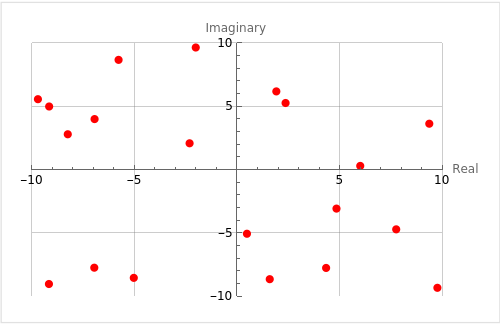
\includegraphics{complexplane.png}
    \caption{Complex Plane}
\end{figure}

\begin{definition}[Complex Plane]
    The complex plane is a two-dimensional space where each point represents a complex number. The horizontal axis represents the real part of the number, and the vertical axis represents the imaginary part. This allows for a geometric interpretation of complex numbers.
\end{definition}
Now that we have point representation on the complex plane, we can gauge the length of a complex number, which we call
\textbf{absolute value} or \textbf{modulus}, as what we do to vectors.
\begin{definition}[Modulus of Complex Number]
    The absolute value or modulus of the number \( z = a + bi \) is denoted by \( |z| \) and is given by
\[ |z| := \sqrt{a^2 + b^2}. \]
\end{definition}
In particular,
\[ |0| = 0, \quad \left|\frac{i}{2}\right| = \frac{1}{2}, \quad |3 - 4i| = \sqrt{9 + 16} = 5. \]
Similarly, we can also gain the distance between two complex numbers in the plane by taking them as two points.
\begin{definition}[Distance between Complex Number]
    Let \( z_1 = a_1 + b_1i \) and \( z_2 = a_2 + b_2i \). 
    \begin{equation}
        |z_1 - z_2| = |(a_1 - a_2) + (b_1 - b_2)i| = \sqrt{(a_1 - a_2)^2 + (b_1 - b_2)^2}
    \end{equation}
\end{definition}
We can use this property to describe curves in the plane.
\begin{example}
    Draw the area that satisfies $|z-z_0|=1$, where $z_0 = 2+2i$.
\end{example}

This set consists of all points $z$ whose distance from $z_0$ is $r$.
\begin{figure}[H]
    \centering
    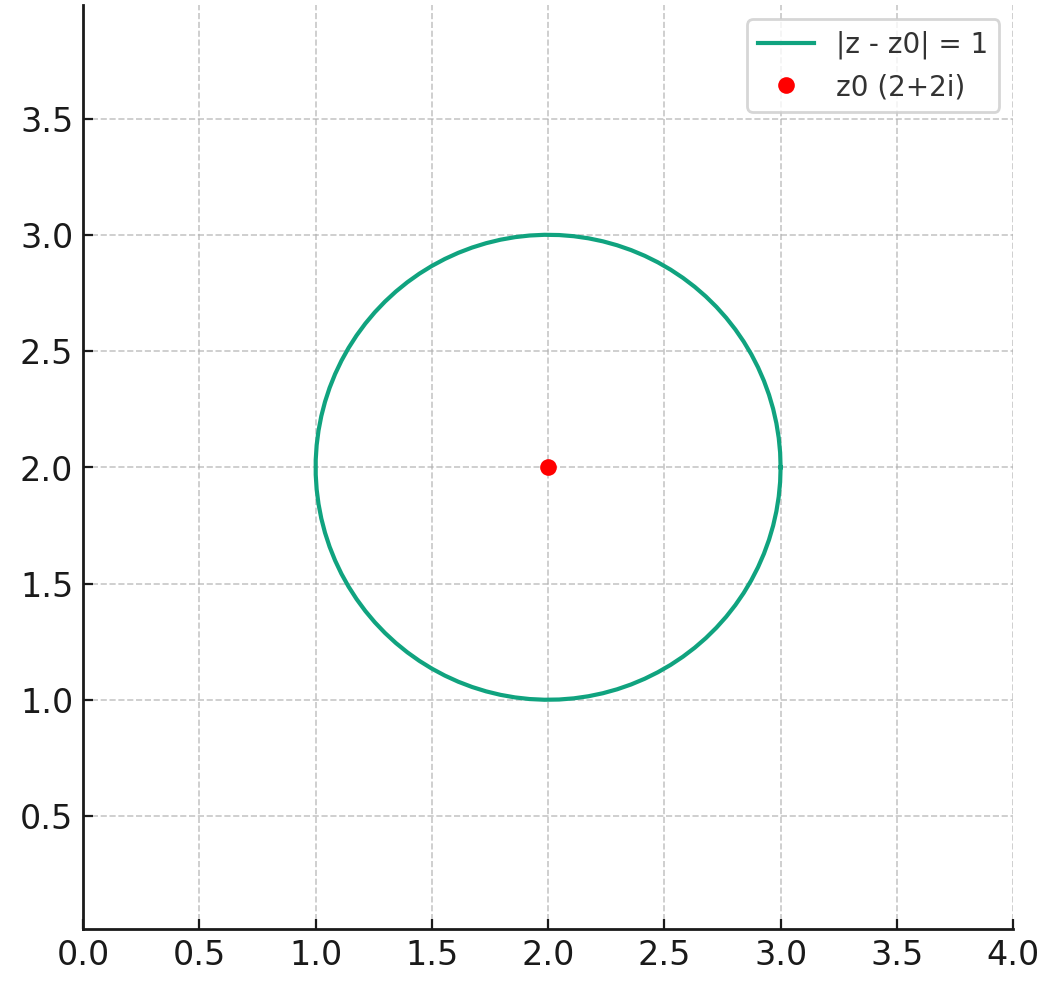
\includegraphics[width = 0.5\textwidth]{locus1.png}
\end{figure}
\begin{example}
    Describe the set of points \( z \) that satisfy the equations

\begin{enumerate}
\item[(a)] \( |z + 2| = |z - 1| \),
\item[(b)] \( |z - 1| = \text{Re} \, z + 1 \).
\end{enumerate}
\end{example}
\textbf{Solution.}

\begin{itemize}
    \item[(a)] A point \( z \) satisfies Eq. (a) if and only if it is equidistant from the points \( -2 \) and \( 1 \). Hence, Eq. (a) is the equation of the perpendicular bisector of the line segment joining \( -2 \) and \( 1 \); that is, Eq. (a) describes the line \( x = -\frac{1}{2} \).

    A more routine method for solving Eq. (a) is to set \( z = x + iy \) in the equation and perform the algebra:
    \begin{align*}
        |z + 2| &= |z - 1|, \\
        |x + iy + 2| &= |x + iy - 1|, \\
        (x + 2)^2 + y^2 &= (x - 1)^2 + y^2, \\
        4x + 4 &= -2x + 1, \\
        x &= -\frac{1}{2}.
    \end{align*}

    \item[(b)] The geometric interpretation of Eq. (b) is less obvious, so we proceed directly with the mechanical approach and derive
    $$\sqrt{(x-1)^2} + y^2 = x+1 \iff y^2 = 4x$$
    which is a parabola.
\end{itemize}
Another important concept is \textbf{complex conjugate}.

Geometrically, the conjugate of a complex number is its reflection on the x-axis.
\begin{wrapfigure}{r}{0.5\textwidth}
    \centering
    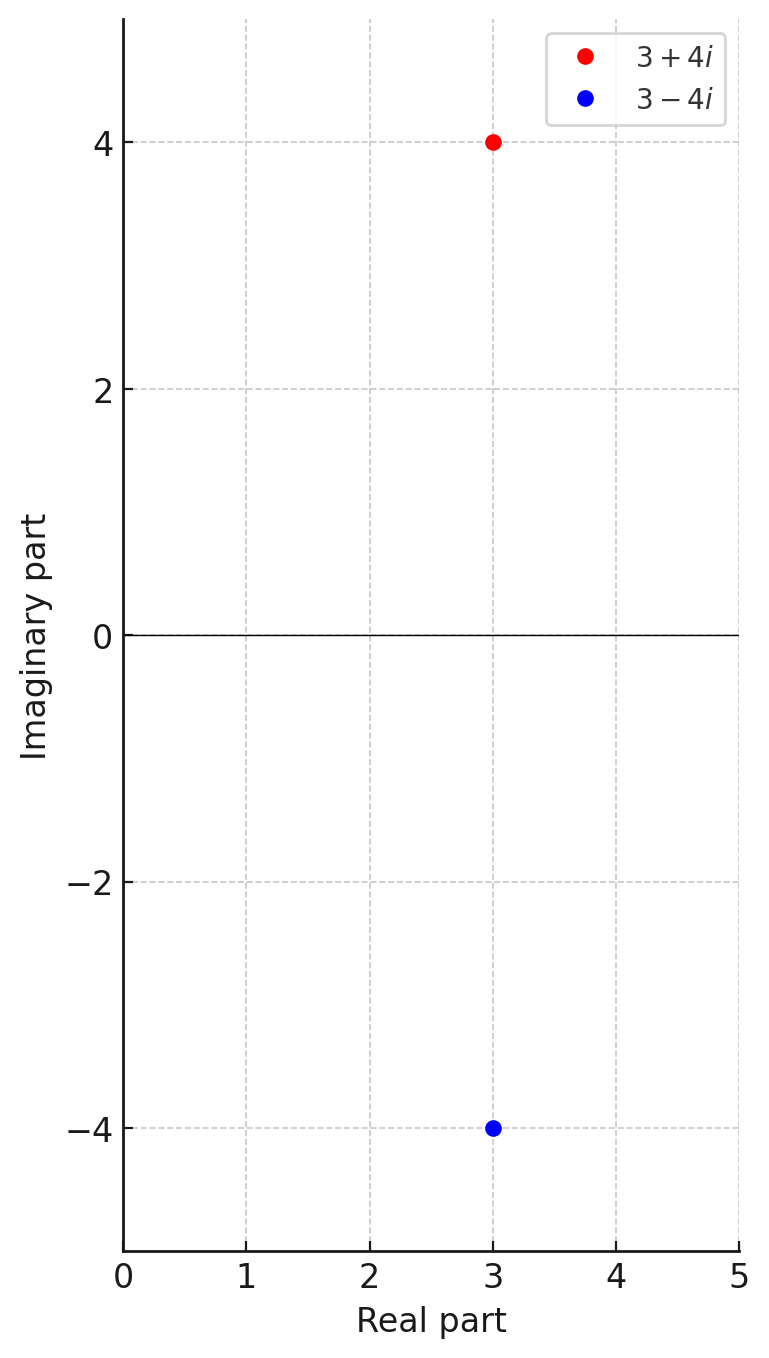
\includegraphics[width=0.48\textwidth]{conjugate.png}
    \caption{Complex Conjugate}
  \end{wrapfigure}
  The complex conjugate of the number $z = a+bi$ is denoted by $\bar{z} = a-bi $.
  It follows that \( z = \bar{z} \) if and only if \( z \) is a real number. Also, it is clear that the conjugate of the sum (difference) of two complex numbers is equal to the sum (difference) of their conjugates; that is,

$$z_1 + z_2 = \bar{z}_1 + \bar{z}_2$$

$$\quad z_1 - z_2 = \bar{z}_1 - \bar{z}_2$$

We also have:
$$\bar{(z_1z_2)} = \bar{z_1} \bar{z_2}$$
and
$$\begin{aligned}\overline{\left(\frac{z_1}{z_2}\right)}&=\frac{\bar{z_1}}{\bar{z_2}}\quad(z_2\neq0);\\\operatorname{Re}z&=\frac{z+\bar{z}}2;\\\operatorname{Im}z&=\frac{z-\bar{z}}{2i};\end{aligned}$$
The proof is not very complex, and is therefore exercises for this section.
\\
\subsection{Exercises}


\begin{exercise}
    Describe the set of points \( z \) in the complex plane that satisfies each of the following.
    \begin{enumerate}
        \item[\textbf{(a)}] \( \text{Im} \, z = -2 \)
        \item[\textbf{(b)}] \( |z - 1 + i| = 3 \)
        \item[\textbf{(c)}] \( |2z - i| = 4 \)
        \item[\textbf{(d)}] \( |z - 1| = |z + i| \)
        \item[\textbf{(e)}] \( |z| = \text{Re} \, z + 2 \)
        \item[\textbf{(f)}] \( |z - 1| + |z + 1| = 7 \)
        \item[\textbf{(g)}] \( |z| = 3|z - 1| \)
        \item[\textbf{(h)}] \( \text{Re} \, z \geq 4 \)
        \item[\textbf{(i)}] \( |z - i| < 2 \)
        \item[\textbf{(j)}] \( |z| > 6 \)
      \end{enumerate}
\end{exercise}
\begin{proof}
    Here we describe the set of points \( z \) in the complex plane that satisfies each of the following conditions:
    
    \begin{enumerate}
      \item[\textbf{(a)}] For \( \text{Im} \, z = -2 \), the Cartesian equation is \( y = -2 \).
      \item[\textbf{(b)}] For \( |z - 1 + i| = 3 \), the Cartesian equation is \( (x - 1)^2 + (y + 1)^2 = 9 \).
      \item[\textbf{(c)}] For \( |2z - i| = 4 \), the Cartesian equation is \( (2x)^2 + (2y - 1)^2 = 16 \).
      \item[\textbf{(d)}] For \( |z - 1| = |z + i| \), the Cartesian equation is \( (x - 1)^2 + y^2 = x^2 + (y + 1)^2 \).
      \item[\textbf{(e)}] For \( |z| = \text{Re} \, z + 2 \), the Cartesian equation is \( x^2 + y^2 = x + 2 \).
      \item[\textbf{(f)}] For \( |z - 1| + |z + 1| = 7 \), this is the equation of an ellipse with foci at (1,0) and (-1,0).
      \item[\textbf{(g)}] For \( |z| = 3|z - 1| \), the Cartesian equation is \( x^2 + y^2 = 3(\sqrt{(x - 1)^2 + y^2}) \).
      \item[\textbf{(h)}] For \( \text{Re} \, z \geq 4 \), the Cartesian equation is \( x \geq 4 \).
      \item[\textbf{(i)}] For \( |z - i| < 2 \), the Cartesian equation is \( (x)^2 + (y - 1)^2 < 4 \).
      \item[\textbf{(j)}] For \( |z| > 6 \), the Cartesian equation is \( x^2 + y^2 > 36 \).
    \end{enumerate}
    \end{proof}

    \begin{exercise}
        Prove that if \( \overline{z}^2 = z^2 \), then \( z \) is either real or pure imaginary.
        \end{exercise}
        
        \begin{proof}
        Let \( z = a + bi \) where \( a \) and \( b \) are real numbers and \( i \) is the imaginary unit. Then \( \overline{z} = a - bi \). 
        
        According to the premise:
        \[ \overline{z}^2 = (a - bi)^2 = a^2 - 2abi + b^2i^2 = a^2 - 2abi - b^2 \]
        \[ z^2 = (a + bi)^2 = a^2 + 2abi + b^2i^2 = a^2 + 2abi - b^2 \]
        
        For \( \overline{z}^2 \) to equal \( z^2 \), the real parts and the imaginary parts of \( \overline{z}^2 \) and \( z^2 \) must be equal, thus:
        \[ a^2 - b^2 = a^2 - b^2 \]
        \[ -2ab = 2ab \]
        
        The real parts are already equal. For the imaginary parts to be equal, \( -2ab \) must equal \( 2ab \), which is only possible if \( ab = 0 \). This means that either \( a = 0 \) or \( b = 0 \) (or both).
        
        If \( a = 0 \), then \( z \) is pure imaginary. If \( b = 0 \), then \( z \) is real. Hence, if \( \overline{z}^2 = z^2 \), \( z \) must be either real or pure imaginary.
        \end{proof}

        \begin{exercise}
            Show that:
            \begin{itemize}
                \item$\lvert z_1z_2 \rvert = \lvert z_1 \rvert \lvert z_2 \rvert$ \quad (the modulus of a product is the product of the moduli)
                \item $\left\lvert \frac{z_1}{z_2} \right\rvert = \frac{\lvert z_1 \rvert}{\lvert z_2 \rvert}$ \quad (the modulus of a quotient is the quotient of the moduli)
                \item $\lvert z_1 \rvert + \lvert z_2 \rvert \leq \lvert z_1 + z_2 \rvert$ \quad (triangle inequality)
              \end{itemize}
        \end{exercise}
        
        \begin{exercise}
            Show that:
            \begin{itemize}
                \item $z_1 + z_2 = \overline{z_1} + \overline{z_2}$
                \item $z_1z_2 = \overline{z_1} \, \overline{z_2}$
                \item $\overline{z}z = \lvert z \rvert^2$
                \item $z + \overline{z} = 2Re(z)$
                \item $kz = \overline{kz}$, for $k \in \mathbb{R}$
              \end{itemize}
        \end{exercise}
        \begin{exercise}
            Prove that \( \overline{z}^k = (\overline{z^k}) \) for every integer \( k \) (provided \( z \neq 0 \) when \( k \) is negative).
            \end{exercise}
            
            \begin{proof}
            Consider a complex number \( z = a + bi \), where \( a \) and \( b \) are real numbers and \( i \) is the imaginary unit. The complex conjugate of \( z \) is \( \overline{z} = a - bi \).
            
            The statement is trivially true for \( k = 0 \) and \( k = 1 \). Now let \( k \) be any positive integer.
            
            We proceed by induction on \( k \):
            
            \textbf{Base case} (\( k = 1 \)):
            \[ \overline{z}^1 = \overline{z} = a - bi = \overline{z^1} \]
            The base case holds.
            
            \textbf{Inductive step}:
            Assume the statement is true for \( k \), i.e., \( \overline{z}^k = \overline{z^k} \). We need to show that \( \overline{z}^{k+1} = \overline{z^{k+1}} \).
            \[ \overline{z}^{k+1} = \overline{z}^k \cdot \overline{z} = \overline{z^k} \cdot \overline{z} \]
            Using the property of complex conjugates that \( \overline{zw} = \overline{z} \cdot \overline{w} \), we have:
            \[ \overline{z^k} \cdot \overline{z} = \overline{z^k \cdot z} = \overline{z^{k+1}} \]
            This completes the inductive step.
            
            For negative integers \( k \), we have \( \overline{z}^k = \overline{z^{-k}} = (\overline{z^{-1}})^k = (\overline{z})^k \), since the complex conjugate of a reciprocal is the reciprocal of the complex conjugate, and the induction hypothesis applies.
            
            Therefore, \( \overline{z}^k = (\overline{z^k}) \) for every integer \( k \).
            \end{proof}

            \begin{exercise}\label{conjugate root}
                Let \( a_1, a_2, \ldots, a_n \) be real constants. Show that if \( z_0 \) is a root of the polynomial equation \( z^n + a_1z^{n-1} + a_2z^{n-2} + \ldots + a_n = 0 \), then so is \( \overline{z_0} \).
                \end{exercise}
                
                \begin{proof}
                Suppose \( z_0 \) is a root of the polynomial \( P(z) = z^n + a_1z^{n-1} + a_2z^{n-2} + \ldots + a_n \). This means that:
                \[ P(z_0) = z_0^n + a_1z_0^{n-1} + a_2z_0^{n-2} + \ldots + a_n = 0 \]
                
                Taking the complex conjugate of the entire equation, we have:
                \[ \overline{P(z_0)} = \overline{z_0^n + a_1z_0^{n-1} + a_2z_0^{n-2} + \ldots + a_n} = \overline{0} \]
                
                Since the \( a_i \) are real, \( \overline{a_i} = a_i \), and using the property that \( \overline{z + w} = \overline{z} + \overline{w} \) and \( \overline{zw} = \overline{z}\cdot \overline{w} \), we get:
                \[ \overline{P(z_0)} = \overline{z_0}^n + a_1\overline{z_0}^{n-1} + a_2\overline{z_0}^{n-2} + \ldots + a_n \]
                
                Since \( \overline{0} = 0 \), the equation simplifies to:
                \[ P(\overline{z_0}) = \overline{z_0}^n + a_1\overline{z_0}^{n-1} + a_2\overline{z_0}^{n-2} + \ldots + a_n = 0 \]
                
                Therefore, \( \overline{z_0} \) is also a root of the polynomial \( P(z) \).
                \end{proof}
                \begin{remark}
                    This statement is actually \textbf{Conjugate Root Theorem}, which we will discuss further details about in finding
                    complex roots of equations.
                \end{remark}
            \begin{exercise}
                We have noted that the conjugate \( \overline{z} \) is the reflection of the point \( z \) in the real axis (the horizontal line \( y = 0 \)). Show that the reflection of \( z \) in the line \( ax + by = c \) (where \( a, b, c \) are real) is given by
\[ \frac{2ic    + (b - ai)\overline{z}}{b + ai} \]
            \end{exercise}
            Hint: In general, the reflection of the point \( (x_1, y_1) \) in the line \( ax + by + c = 0 \) given by this formula:
            \[ 
            x_2 = \frac{x_1(b^2 - a^2) - 2aby_1 - 2ac}{a^2 + b^2}
            \]
            \[ 
            y_2 = \frac{y_1(a^2 - b^2) - 2abx_1 - 2bc}{a^2 + b^2}
            \]
            
            \begin{proof}
                Now the reflection of $z = (x, y)$ in the line $ax + by - c = 0$ is $w = u + iv$, $u, v \in \mathbb{R}$, where:
                \begin{align*}
                u &= \frac{x(b^2 - a^2) - 2aby + 2ac}{a^2 + b^2}, \\
                v &= \frac{y(a^2 - b^2) - 2abx + 2bc}{a^2 + b^2}.
                \end{align*}
                Then:
                \begin{align*}
                w = u + vi &= \frac{x(b^2 - a^2) - 2aby + 2ac}{a^2 + b^2} + \frac{y(a^2 - b^2) - 2abx + 2bc}{a^2 + b^2}i. 
                \end{align*}
                Next, we'll prove now:
                \begin{align*}
                w &= \frac{2ic + (b - ai)\overline{z}}{b + ai}.
                \end{align*}
                We'll factorize and simplify $w$ in $(*)$:
                \begin{align*}
                w &= \frac{x(b^2 - a^2) - 2aby + 2ac}{a^2 + b^2} + \frac{y(a^2 - b^2) - 2abx + 2bc}{a^2 + b^2}i \\
                &= \frac{x(b^2 - a^2) - 2aby + 2ac + y(a^2 - b^2)i - 2abxi + 2bci}{a^2 + b^2}.
                \end{align*}
                Simplify more:
                \begin{align*}
                (b^2 - a^2 - 2abi) &= (b - ai)^2, \\
                (a^2i - b^2i - 2ab) &= (-i)(b^2 - a^2 + 2ab) \\
                &= (-i)(b + ai)^2 \quad \left(\text{since } \frac{1}{i} = -i\right), \\
                &= (-i)(b - ai)(b + ai)^2 \\
                &= i(b - ai) \\
                &= i(b - ai)(b + ai).
                \end{align*}
                Now we'll put all of them in the $(1)$,
                \begin{align*}
                w &= \frac{x(b - ai)^2 - yi(b - ai)^2 + 2ci(b - ai)}{b + ai} \\
                &= \frac{(b - ai)x(b - ai) - yi(b - ai) + 2ci}{b + ai} \\
                &= \frac{2ci + (b - ai)\overline{z}}{b + ai}.
                \end{align*}
                Therefore, the reflection of $z$ in the line $ax + by = c$ is:
                \begin{align*}
                w &= \frac{2ic + (b - ai)\overline{z}}{b + ai}.
                \end{align*}
                \end{proof}
               
\section{Vector and Polar Form}
\subsection{Vector Form of Complex Number}
Now that we can express complex numbers as points scattered in the complex plane, we can take them as direction vectors
in the plane as shown in figure \ref{vec}. 
\begin{figure}[H]
    \centering \label{vec}
    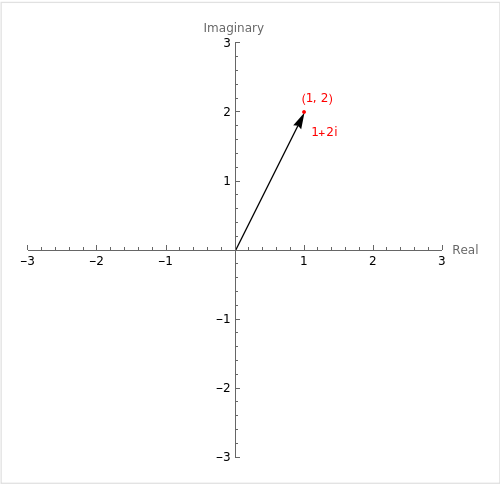
\includegraphics[width = 0.5\textwidth]{complexvector.png}
    \caption{Complex Number as Vector}
\end{figure}
With this, we can apply all possible operations of vectors to complex numbers, such as the \textbf{parallelogram law} as in figure \ref{parrl}.
\begin{figure}[H]
    \centering \label{parrl}
    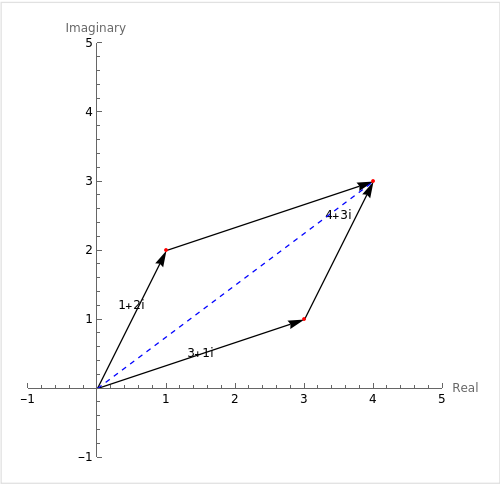
\includegraphics[width = 0.5\textwidth]{paralaw.png}
    \caption{Parallelogram Law}
\end{figure}
Examing this figure, it actually reminds us of a important conclusion mentioned in earlier chapter. If we focus on
the lower triangle of the parallelogram, and denote these two complex numbers as $z_1$ and $z_2$ respectively.
They hold that: $$|z_1+z_2| \leq |z_1|+|z_2|$$
This is exactly the geometrical meaning of triangular inequality as in definition \ref{triangularineq}.
And these are all we need to know about complex number's vector form, as it is not used very common.

\subsection{Polar Form of Complex Number}
This section discusses one of the most commonly used form of complex number. We start with introducing a new coordinate syste.

\subsubsection{The Polar Coordinate}
Polar coordinates provide an alternative to Cartesian coordinates for describing the location of points in a two-dimensional plane. While Cartesian coordinates use a grid of horizontal and vertical lines to specify a point by its horizontal (x) and vertical (y) distances from an origin, polar coordinates specify a point by its distance from a reference point (called the pole, analogous to the origin) and an angle relative to a reference direction.
\begin{figure}[H]
    \centering \label{polar}
    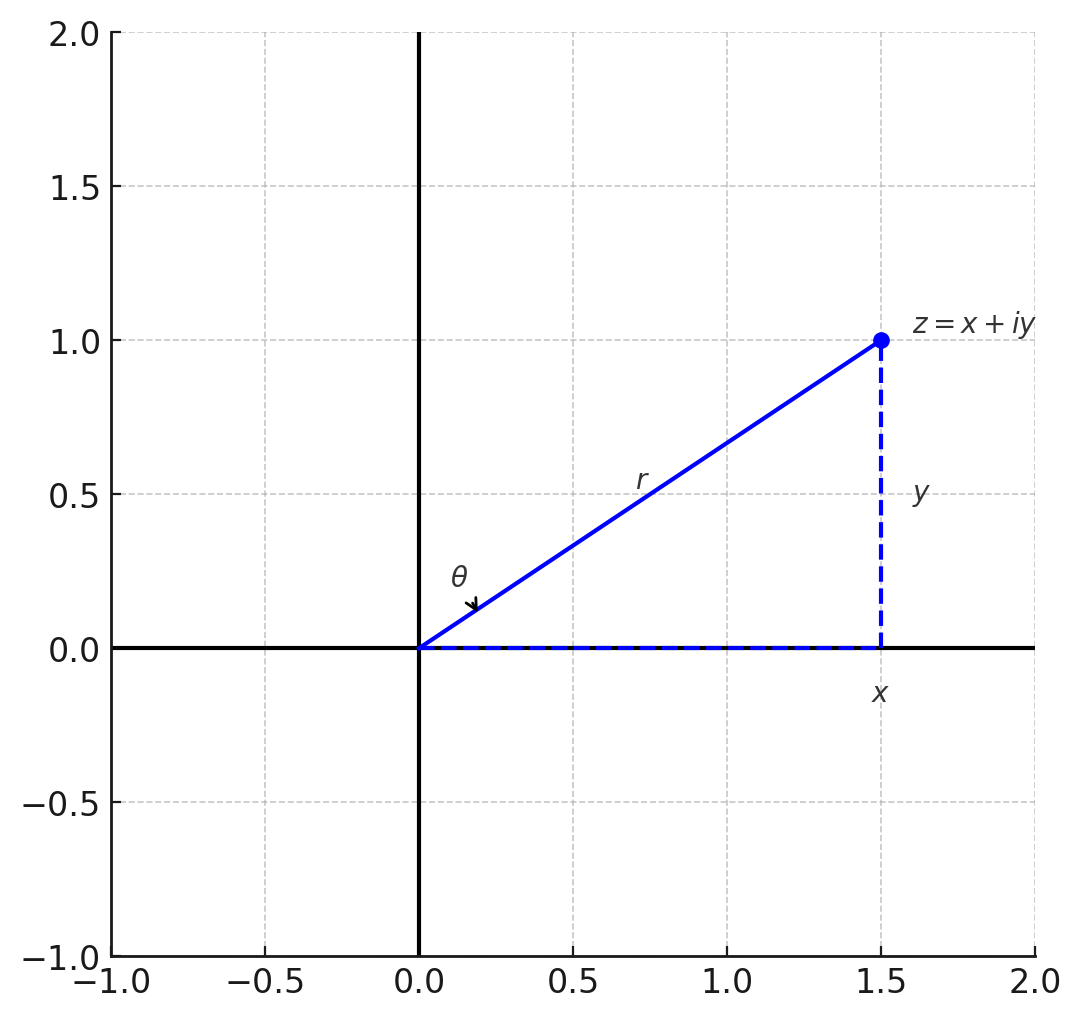
\includegraphics[width = 0.5\textwidth]{polar2.png}
    \caption{Complex Number in Polar Coordinate}
\end{figure}
A point's location in polar coordinates is given as \( (r, \theta) \), where \( r \) is the radial distance from the pole, and \( \theta \) is the angular coordinate, typically measured in radians from the positive x-axis (the reference direction). Polar coordinates are particularly useful in situations where the geometry of a problem has rotational symmetry, making it more natural and simpler to work with angles and radii than with rectangular coordinates.

One of the most common applications of polar coordinates is in the field of trigonometry, complex numbers, and vector calculus, where they provide a more straightforward approach to solving problems involving circular motion, periodic functions, and fields.

\subsubsection{Polar Expression of Complex Number}
Now that we know the existence of polar form, how can we get it from Cartesian form? In the Cartesian coordinate,
the positions are expressed, straightforwardly, in the horizontal and vertical distance to y and x-axis, while in polar
coordinate, we express them using the angle between the line from the origin to the specific position and the horizontal axis, as well
as the length of this line. Is there a mapping or relation between the points in these two types of coordinates? Some clever students
may have noticed that trigonometric functions are the keys here.
we readily derive the equations expressing the rectangular (or Cartesian) coordinates $(x, y)$ in terms of the polar coordinates $(r, \theta)$:
\begin{equation}
x = r \cos \theta, \quad y = r \sin \theta. 
\end{equation}
On the other hand, the expressions for $(r, \theta)$ in terms of $(x, y)$ contain some minor but troublesome complications. Indeed the coordinate $r$ is given, unambiguously, by
\begin{equation}
r = \sqrt{x^2 + y^2} = |z|. 
\end{equation}

However, observe that although it is certainly true that $\tan \theta = \frac{y}{x}$, the natural conclusion
\begin{equation}
\theta = \tan^{-1}\left(\frac{y}{x}\right)
\end{equation}
is \textit{invalid} for points $z$ in the second and third quadrants (since the standard interpretation of the arctangent function places its range in the first and fourth quadrants). Since an angle is fixed by its sine \textit{and} cosine, $\theta$ is uniquely determined by the pair of equations
\begin{equation}
\cos \theta = \frac{x}{|z|}, \quad \sin \theta = \frac{y}{|z|}, 
\end{equation}
And all these lead us to the polar form of a given complex number:
\begin{equation}
    z=x+iy=r(\cos\theta+i\sin\theta)=r\operatorname{cis}\theta
\end{equation}

Considering the circularity of radiant, we introduce the \textbf{argument} of complex number.
\begin{definition}[Arguement of Complex Number] \label{polarform}
In the study of complex numbers, the \emph{argument} of a complex number \( z \), denoted as \( \text{arg}(z) \), is a fundamental concept representing the angle between the positive real axis and the line segment that joins the origin with the point \( z \) in the complex plane. Specifically, if \( z = x + iy \), where \( x \) and \( y \) are real numbers, then \( \text{arg}(z) \) is defined as the angle \( \theta \) in polar coordinates that satisfies \( x = r\cos(\theta) \) and \( y = r\sin(\theta) \), where \( r \) is the magnitude of \( z \). The value of \( \text{arg}(z) \) is usually given in radians and, by convention, is restricted to the interval \( (-\pi, \pi] \), known as the principal value. The argument provides a complete description of the direction in which the point \( z \) lies from the origin, serving as a crucial tool in the fields of complex analysis, phasor calculus in electrical engineering, and in the representation of waves and oscillations.
\end{definition}

\begin{example}
    Find $\arg(1 + \sqrt{3}i)$ and write $1 + \sqrt{3}i$ in polar form.
\end{example}
\textbf{Solutions:}

Note that $r = |1 + \sqrt{3}i| = 2$ and that the equations $\cos\theta = \frac{1}{2}$, $\sin\theta = \frac{\sqrt{3}}{2}$ are satisfied by $\theta = \frac{\pi}{3}$. Hence $\arg(1 + \sqrt{3}i) = \frac{\pi}{3} + 2k\pi, k = 0, \pm1, \pm2, \ldots$ [in particular, $\text{Arg}(1 + \sqrt{3}i) = \frac{\pi}{3}$]. The polar form of $1 + \sqrt{3}i$ is
\[2(\cos\frac{\pi}{3} + i\sin\frac{\pi}{3}) = 2\operatorname{cis}\frac{\pi}{3}.\]

More properties of polar form complex number could be derived with properties of trigonometric identities.
Now suppose we have 
$$z_1=r_1\left(\cos\theta_1+i\sin\theta_1\right),\quad z_2=r_2\left(\cos\theta_2+i\sin\theta_2\right)$$
then we have
$$z_1z_2=r_1r_2\left[(\cos\theta_1\cos\theta_2-\sin\theta_1\sin\theta_2)+i(\sin\theta_1\cos\theta_2+\cos\theta_1\sin\theta_2)\right]$$
which follows that
\begin{equation} \label{polarprod}
    z_1z_2=r_1r_2\left[\cos\left(\theta_1+\theta_2\right)+i\sin\left(\theta_1+\theta_2\right)\right]
\end{equation}

\begin{remark}
The compound angle formula is applied in the proof, which should already been covered in high school
syllabus. You may refer to \href{https://en.wikipedia.org/wiki/List_of_trigonometric_identities}{this link} for further information.
A concise proof is provided below.
\begin{proof}[Proof of the Composite Angle Formulas]
    To prove the sine of the sum of two angles \( \alpha \) and \( \beta \), we can use the unit circle and the definition of sine and cosine.
    
    Consider a unit circle where point \( A \) corresponds to angle \( \alpha \), and point \( B \) corresponds to angle \( \alpha + \beta \). Point \( A \) has coordinates \( (\cos(\alpha), \sin(\alpha)) \), and point \( B \) has coordinates \( (\cos(\alpha + \beta), \sin(\alpha + \beta)) \).
    
    By rotating point \( A \) by angle \( \beta \), we can form a right triangle where the new point, \( C \), has coordinates \( (\cos(\alpha)\cos(\beta) - \sin(\alpha)\sin(\beta), \sin(\alpha)\cos(\beta) + \cos(\alpha)\sin(\beta)) \).
    
    The coordinates of point \( C \) represent the cosine and sine of the sum of angles \( \alpha \) and \( \beta \) due to the rotation. Therefore, we have:
    
    \[
    \sin(\alpha + \beta) = \sin(\alpha)\cos(\beta) + \cos(\alpha)\sin(\beta)
    \]
    \[
    \cos(\alpha + \beta) = \cos(\alpha)\cos(\beta) - \sin(\alpha)\sin(\beta)
    \]
    
    Similarly, by considering the rotation in the opposite direction (subtracting angle \( \beta \) from \( \alpha \)), we can derive the formulas for the sine and cosine of the difference of two angles:
    
    \[
    \sin(\alpha - \beta) = \sin(\alpha)\cos(\beta) - \cos(\alpha)\sin(\beta)
    \]
    \[
    \cos(\alpha - \beta) = \cos(\alpha)\cos(\beta) + \sin(\alpha)\sin(\beta)
    \]
    
    Thus, we have proven the composite angle formulas for sine and cosine.

    \end{proof}
\end{remark}

The abbreviated version of Eq. \ref{polarprod} reads as follows:
\[
\overline{z_1z_2} = (r_1 \operatorname{cis} \theta_1)(r_2 \operatorname{cis} \theta_2) = (r_1r_2) \operatorname{cis} (\theta_1 + \theta_2)
\]
and we see that

\textbf{The modulus of the product is the product of the moduli:}
\[
|\overline{z_1z_2}| = |z_1||z_2| \quad (= r_1r_2);
\]


\textbf{The argument of the product is the sum of the arguments:}
\[
\arg \overline{z_1z_2} = \arg z_1 + \arg z_2 \quad (= \theta_1 + \theta_2).
\]
As division is the inverse of multiplication, we can get the following statements by similar method:
\begin{equation} \label{5.8}
    \frac{z_{1}}{z_{2}}=\frac{r_{1}}{r_{2}}\left[\cos\left(\theta_{1}-\theta_{2}\right)+i\sin\left(\theta_{1}-\theta_{2}\right)\right]=\frac{r_{1}}{r_{2}}\mathrm{cis}\left(\theta_{1}-\theta_{2}\right)
\end{equation}
\begin{equation}\label{5.9}
    \arg\left(\frac{z_{1}}{z_{2}}\right)=\arg z_{1}-\arg z_{2} 
\end{equation}
\begin{equation}\label{5.10}
    \left|\frac{z_1}{z_2}\right|=\frac{|z_1|}{|z_2|}
\end{equation}
\begin{example}
    Write the quotient \( \frac{(1 + i)}{(\sqrt{3} - i)} \) in polar form.
\end{example}
\begin{proof}
    The polar forms for \( 1 + i \) and \( \sqrt{3} - i \) are
    \[
    1 + i = |1 + i| \operatorname{cis}(\arg(1 + i)) = \sqrt{2} \operatorname{cis}\left(\frac{\pi}{4}\right),
    \]
    \[
    \sqrt{3} - i = 2 \operatorname{cis}\left(-\frac{\pi}{6}\right).
    \]
    Hence, from Eq. \ref{5.8}, we have
    \[
    \frac{1 + i}{\sqrt{3} - i} = \frac{\sqrt{2}}{2} \operatorname{cis} \left(\frac{\pi}{4} - \left(-\frac{\pi}{6}\right)\right) = \frac{\sqrt{2}}{2} \operatorname{cis}\left(\frac{5\pi}{12}\right).
    \]
    \end{proof}

\subsection{Exercises}
\begin{exercise}
    Find the following:
    \begin{enumerate}
        \item[(a)] \( \left| \frac{1 + 2i}{-2 - i} \right| \)
        \item[(b)] \( \left| (1 + i)(2 - 3i)(4i - 3) \right| \)
        \item[(c)] \( \left| \frac{i(2 + i)^3}{(1 - i)^2} \right| \)
        \item[(d)] \( \left| \frac{(\pi + i)^{100}}{(\pi - i)^{100}} \right| \)
    \end{enumerate}
\end{exercise}
\begin{exercise}
    Draw the following vectors:
    \begin{enumerate}
        \item[(a)] \( 7 \operatorname{cis}\left(\frac{3\pi}{4}\right) \)
        \item[(b)] \( 4 \operatorname{cis}\left(-\frac{\pi}{6}\right) \)
        \item[(c)] \( \operatorname{cis}\left(\frac{3\pi}{4}\right) \)
        \item[(d)] \( 3 \operatorname{cis}\left(\frac{27\pi}{4}\right) \)
    \end{enumerate}
\end{exercise}
\begin{exercise}
    Find the argument of each of the following complex numbers and write each in polar form:
    \begin{enumerate}
        \item[(a)] \( -\frac{1}{2} \)
        \item[(b)] \( -3 + 3i \)
        \item[(c)] \( -\pi i \)
        \item[(d)] \( -2\sqrt{3} - 2i \)
        \item[(e)] \( (1 - i)(-\sqrt{3} + i) \)
        \item[(f)] \( (\sqrt{3} - i)^2 \)
        \item[(g)] \( \frac{-1 + \sqrt{3}i}{2 + 2i} \)
        \item[(h)] \( \frac{-\sqrt{7}(1 + i)}{\sqrt{3} + i} \)
    \end{enumerate}
\end{exercise}
\begin{exercise}
    Show geometrically that the nonzero complex numbers \( z_1 \) and \( z_2 \) satisfy \( z_1 + z_2 = |z_1| + |z_2| \) if and only if they have the same argument.
\end{exercise}
\begin{proof}
    If \( z_1 \) and \( z_2 \) have the same argument, it follows that:

    We see here if $z_1 = r_1(\cos \theta + i \sin \theta)$, $z_2 = r_2(\cos \theta + i \sin \theta)$, then
\begin{align*}
|z_1 + z_2| &= |r_1(\cos \theta + i \sin \theta) + r_2(\cos \theta + i \sin \theta)| \\
&= |(r_1 + r_2)(\cos \theta + i \sin \theta)| \\
&= r_1 + r_2 = |z_1| + |z_2|
\end{align*}
\end{proof}
\begin{exercise}
    Given the vector \( z \), interpret geometrically the vector \( (\cos \phi + i \sin \phi)z \).
\end{exercise}
\textbf{Solution:}

Let \( z \in \mathbb{C} \), \( z = r(\cos \theta + i \sin \theta) \)

\[
(\cos \phi + i \sin \phi)z = (\cos \phi + i \sin \phi)r(\cos \theta + i \sin \theta)
\]
\[
= r[\cos(\theta + \phi) + i \sin(\theta + \phi)]
\]
\[
= r\operatorname{cis}(\theta + \phi)
\]

Geometrically this: \( r\operatorname{cis}(\theta + \phi) \) means a vector that its length \( r \) and argument is \( \theta + \phi \), we can get it by rotating vector \( z \) about origin through an angle \( \phi \) in the counterclockwise direction.

\begin{exercise}
    Show that $|z_1z_2z_3|=|z_1||z_2||z_3|$ and thus prove 
    $$|\prod_{i=1}^{n} z_i| = \prod_{i=1}^{n} |z_i|$$
    \begin{remark}
        $\prod$ is called pi (upper case) notation. Take it as the sigma notation for multiplication.
    \end{remark}
\end{exercise}
    \begin{proof}
        Consider the complex numbers \( z_1 = r_1(\cos \theta_1 + i\sin \theta_1) \), \( z_2 = r_2(\cos \theta_2 + i\sin \theta_2) \), and \( z_3 = r_3(\cos \theta_3 + i\sin \theta_3) \), where \( r_1, r_2, \) and \( r_3 \) are the moduli of \( z_1, z_2, \) and \( z_3 \) respectively, and \( \theta_1, \theta_2, \) and \( \theta_3 \) are the arguments. The product \( z_1z_2z_3 \) is then given by:
        \[
        z_1z_2z_3 = r_1r_2r_3(\cos(\theta_1 + \theta_2 + \theta_3) + i\sin(\theta_1 + \theta_2 + \theta_3))
        \]
        
        The modulus of this product is:
        \[
        |z_1z_2z_3| = |r_1r_2r_3(\cos(\theta_1 + \theta_2 + \theta_3) + i\sin(\theta_1 + \theta_2 + \theta_3))| = r_1r_2r_3
        \]
        
        Since the moduli of \( z_1, z_2, \) and \( z_3 \) are \( r_1, r_2, \) and \( r_3 \) respectively, it follows that:
        \[
        |z_1z_2z_3| = |z_1||z_2||z_3|
        \]
        
        Now, extend this property to a product of \( n \) complex numbers:
        \[
        \prod_{i=1}^{n} z_i = \prod_{i=1}^{n} r_i(\cos \theta_i + i\sin \theta_i)
        \]
        
        Taking the modulus of both sides:
        \[
        \left|\prod_{i=1}^{n} z_i\right| = \left|\prod_{i=1}^{n} r_i(\cos \theta_i + i\sin \theta_i)\right| = \prod_{i=1}^{n} r_i
        \]
        
        Thus:
        \[
        \prod_{i=1}^{n} |\overline{z_i}| = \prod_{i=1}^{n} |z_i|
        \]
        
        as required.

        MI is also a option:

        \textbf{Base case} (\(n = 1\)): For a single complex number \(z_1\), the statement is trivially true since \(|\overline{z_1}| = |z_1|\).

        \textbf{Inductive step}: Assume the statement holds for \(n = k\), i.e.,
        \[
        \prod_{i=1}^{k} |\overline{z_i}| = \prod_{i=1}^{k} |z_i|
        \]
        Now consider \(n = k + 1\) complex numbers. By the induction hypothesis and the property that the modulus of a product is equal to the product of the moduli for any two complex numbers \(a\) and \(b\), namely \(|ab| = |a||b|\), we have:
        \[
        \prod_{i=1}^{k+1} |\overline{z_i}| = |\overline{z_{k+1}}| \prod_{i=1}^{k} |\overline{z_i}| = |z_{k+1}| \prod_{i=1}^{k} |z_i| = \prod_{i=1}^{k+1} |z_i|
        \]
        Thus, by mathematical induction, the statement is proved for all \(n \in \mathbb{N}\).
        \end{proof}

    \begin{exercise}
        Show that\begin{enumerate}
            \item[(a)] $\text{arg } z_1z_2z_3 = \text{arg } z_1 + \text{arg } z_2 + \text{arg } z_3$
            \item[(b)] $\text{arg } z_1 \overline{z_2} = \text{arg } z_1 - \text{arg } z_2$.
        \end{enumerate}
    \end{exercise}              
    \textbf{Solution:}
    Let $z_1, z_2, z_3 \in \mathbb{C}$,

(a) we'll prove $\text{arg }(z_1z_2z_3) = \text{arg } z_1 + \text{arg } z_2 + \text{arg } z_3$

Let $z_1 = r_1(\cos \theta_1 + i \sin \theta_1)$, where $\text{arg } z_1 = \theta_1$

$z_2 = r_2(\cos \theta_2 + i \sin \theta_2)$, where $\text{arg } z_2 = \theta_2$

$z_3 = r_3(\cos \theta_3 + i \sin \theta_3)$, where $\text{arg } z_3 = \theta_3$

We'll prove $\text{arg } z_1z_2z_3 = \text{arg } z_1 + \text{arg } z_2 + \text{arg } z_3$

At first we'll find $z_1z_2z_3$:

\begin{align*}
    z_1z_2z_3 &= (z_1z_2)z_3 = r_1r_2[\cos(\theta_1 + \theta_2) + i \sin(\theta_1 + \theta_2)]z_3 \\
    &= r_1r_2r_3[\cos(\theta_1 + \theta_2) + i \sin(\theta_1 + \theta_2)](\cos \theta_3 + i \sin \theta_3) \\
    &= r_1r_2r_3[\cos(\theta_1 + \theta_2) \cos \theta_3 - \sin(\theta_1 + \theta_2) \sin \theta_3 \\
    &\quad + i(\sin(\theta_1 + \theta_2) \cos \theta_3 + \cos(\theta_1 + \theta_2) \sin \theta_3)] \\
    &= r_1r_2r_3[\cos(\theta_1 + \theta_2 + \theta_3) + i \sin(\theta_1 + \theta_2 + \theta_3)]
\end{align*}

Therefore, $\text{arg } z_1z_2z_3 = \theta_1 + \theta_2 + \theta_3 = \text{arg } z_1 + \text{arg } z_2 + \text{arg } z_3$.

(b) we'll prove $\text{arg } z_1 \overline{z_2} = \text{arg } z_1 - \text{arg } z_2$

Therefore, $z_2 = r_2(\cos \theta_2 + i \sin \theta_2)$ and hence

\[
\overline{z_2} = r_2(\cos(-\theta_2) + i \sin(-\theta_2)) = r_2(\cos \theta_2 - i \sin \theta_2)
\]

Now we find the argument of $z_1 \overline{z_2}$:

\begin{align*}
    \text{arg } z_1 \overline{z_2} &= \text{arg }[(r_1(\cos \theta_1 + i \sin \theta_1))(r_2(\cos \theta_2 - i \sin \theta_2))] \\
    &= \text{arg }[r_1r_2((\cos \theta_1 \cos \theta_2 + \sin \theta_1 \sin \theta_2) \\
    &\quad + i(\cos \theta_1 \sin \theta_2 - \cos \theta_2 \sin \theta_1))] \\
    &= \text{arg }[r_1r_2(\cos(\theta_1 - \theta_2) + i \sin(\theta_1 - \theta_2))] \\
    &= \theta_1 - \theta_2 \\
    &= \text{arg } z_1 - \text{arg } z_2
\end{align*}

Thus, $\text{arg } z_1 \overline{z_2} = \text{arg } z_1 - \text{arg } z_2$.

\begin{exercise}
    Recall that the dot (scalar) product of two planar vectors $v_1 = (x_1, y_1)$ and $v_2 = (x_2, y_2)$ is given by:
    \[ v_1 \cdot v_2 = x_1x_2 + y_1y_2. \]
\textbf{Show that the dot product of the vectors represented by the complex numbers $z_1$ and $z_2$ is given by}
\[ z_1 \cdot z_2 = Re(\overline{z_1}z_2). \]
\end{exercise}
\begin{proof}
    Let $z_1, z_2 \in \mathbb{C}$.

We can represent $z_1, z_2$ as vectors as follows:
\[ z_1 = (x_1, y_1) = x_1 + y_1j, \quad z_2 = (x_2, y_2) = x_2 + y_2j \]
\[ z_1 \cdot z_2 = (x_1 + y_1j) \cdot (x_2 + y_2j) \]
\[ = x_1x_2 + y_1y_2 + x_1y_2(j \cdot j) + x_2y_1(i \cdot j) \]
\[ = x_1x_2 + y_1y_2 + 0 + 0 \quad (\because i^2 = j^2 = -1, i \cdot j = 0) \]
\[ \therefore z_1 \cdot z_2 = x_1x_2 + y_1y_2 \quad \text{(1)} \]

Now we'll find:
\[ \overline{z_1}z_2 = (x_1 - y_1j)(x_2 + y_2j) = x_1x_2 + y_1y_2 + x_1y_2(-j) - x_2y_1j \]
\[ \therefore Re(\overline{z_1}z_2) = x_1x_2 + y_1y_2 \quad \text{(2)} \]

From (1) and (2) we get:
\[ z_1 \cdot z_2 = Re(\overline{z_1}z_2) = x_1x_2 + y_1y_2 \]
\end{proof}

\begin{exercise}
    We have proven the \textbf{Generalized Triangle Inequality} in last chapter that:
    $$\left|\sum_{k=1}^{n} z_{k}\right| \leq \sum_{k=1}^{n}\left|z_{k}\right|$$
    For complex number$z_1$, $z_2$, and $z_3$, prove that:
    $$\left|\frac{m_{1} z_{1}+m_{2} z_{2}+m_{3} z_{3}}{m_{1}+m_{2}+m_{3}}\right| \leq 1$$
\end{exercise}
\begin{proof}
    
We'll take at first:
\[
\left| \frac{m_1z_1 + m_2z_2 + m_3z_3}{m_1 + m_2 + m_3} \right| = \frac{\left| m_1z_1 + m_2z_2 + m_3z_3 \right|}{\left| m_1 + m_2 + m_3 \right|}
\]

Now we'll find:
\[
\left| m_1z_1 + m_2z_2 + m_3z_3 \right| \leq \left| m_1z_1 \right| + \left| m_2z_2 \right| + \left| m_3z_3 \right| \quad \text{(Triangle inequality)}
\]
\[
= m_1 \left| z_1 \right| + m_2 \left| z_2 \right| + m_3 \left| z_3 \right|
\]
\[
\leq m_1 + m_2 + m_3 \quad (\text{since } m_1, m_2, m_3 > 0 \text{ and } \left| z_1 \right|, \left| z_2 \right|, \left| z_3 \right| \leq 1)
\]
\[
= \left| m_1 + m_2 + m_3 \right|
\]

Therefore:
\[
\left| m_1z_1 + m_2z_2 + m_3z_3 \right| \leq \left| m_1 + m_2 + m_3 \right|
\]
\[
\therefore \left| \frac{m_1z_1 + m_2z_2 + m_3z_3}{m_1 + m_2 + m_3} \right| = \frac{\left| m_1z_1 + m_2z_2 + m_3z_3 \right|}{\left| m_1 + m_2 + m_3 \right|} \leq 1
\]
\end{proof}

\section{Exponential Form}
The other form for complex number is its exponential form with base $e$. Euler's formula relate the exponential
expression to the polar expression. However, the proof of Euler's formula require further knowledge of calculus, such as
Taylor series. You may access \href{https://www.youtube.com/watch?v=mvmuCPvRoWQ&t=78s}{this link} for a proof without
calculus. You can also just skip the proof for now, since it does not affect the problem-solving in this chapter.

\begin{definition}[Euler's Formula]
    \begin{equation}
        e^{i y}=\cos y+i \sin y 
    \end{equation}
\end{definition}
You can relate this formula to the polar form very easily, since the right-hand side is equivalent to$cisy$,
which means $y$ is exactly the principal argument of the complex number, $\theta$.

Euler's Formula enables us to write the polar form of a complex number as
\[
z = r \text{cis} \theta = r(\cos \theta + i \sin \theta) = r e^{i\theta}.
\]
Thus, we can (and do) drop the awkward ``cis'' artifice and use, as the standard polar representation,
\[
z = r e^{i\theta} = \lvert z \rvert e^{\text{arg} z}.
\]
In particular, notice the following identities:
\[
e^{i0} = e^{2\pi i} = e^{-2\pi i} = e^{4\pi i} = e^{-4\pi i} = \cdots = 1,
\]
\[
e^{(\pi/2)i} = i, \quad e^{(-\pi/2)i} = -i, \quad e^{\pi i} = -1.
\]

Observe also that  $\left|e^{i \arg z}\right|=1$  and that Euler's equation leads to the following representations of the customary trigonometric functions:
$$\begin{array}{l}
    \cos \theta=\operatorname{Re} e^{i \theta}=\frac{e^{i \theta}+e^{-i \theta}}{2}, \\
    \sin \theta=\operatorname{Im} e^{i \theta}=\frac{e^{i \theta}-e^{-i \theta}}{2 i} .
    \end{array}$$

\begin{proof}
    We start with Euler's formula which states that for any real number \( \theta \),
\begin{equation}
    e^{i\theta} = \cos(\theta) + i\sin(\theta).
\end{equation}
The complex conjugate of \( e^{i\theta} \) is \( e^{-i\theta} \), which gives us
\begin{equation}
    e^{-i\theta} = \cos(-\theta) + i\sin(-\theta) = \cos(\theta) - i\sin(\theta),
\end{equation}
since cosine is an even function, \( \cos(-\theta) = \cos(\theta) \), and sine is an odd function, \( \sin(-\theta) = -\sin(\theta) \).

To derive the expression for the cosine function, we take the sum of \( e^{i\theta} \) and \( e^{-i\theta} \), and divide by 2:
\begin{equation}
    \cos(\theta) = \frac{e^{i\theta} + e^{-i\theta}}{2}.
\end{equation}
This is because the imaginary parts \( i\sin(\theta) \) and \( -i\sin(\theta) \) cancel each other out, leaving the sum of \( \cos(\theta) + \cos(\theta) \), which is then divided by 2.

To derive the expression for the sine function, we take the difference of \( e^{i\theta} \) and \( e^{-i\theta} \), and divide by \( 2i \):
\begin{equation}
    \sin(\theta) = \frac{e^{i\theta} - e^{-i\theta}}{2i}.
\end{equation}
Here, the real parts \( \cos(\theta) - \cos(\theta) \) cancel out, leaving the difference of \( i\sin(\theta) - (-i\sin(\theta)) \) which is \( 2i\sin(\theta) \), and then dividing by \( 2i \) yields \( \sin(\theta) \).

This completes the derivation of the exponential forms of the sine and cosine functions.
\end{proof}

The rules derived in definition \ref{polarform} for multiplying and dividing complex numbers in polar form now find very natural expressions:
\begin{equation}
    z_1z_2 = (r_1e^{i\theta_1})(r_2e^{i\theta_2}) = (r_1r_2)e^{i(\theta_1+\theta_2)},
\end{equation}
\begin{equation}
    \frac{z_1}{z_2} = \frac{r_1e^{i\theta_1}}{r_2e^{i\theta_2}} = \left(\frac{r_1}{r_2}\right)e^{i(\theta_1-\theta_2)},
\end{equation}
and complex conjugation of \( z = re^{i\theta} \) is accomplished by changing the sign of \( i \) in the exponent:
\begin{equation}
    \bar{z} = re^{-i\theta}.
\end{equation}

\begin{example}
    Compute (a) \( \frac{1 + i}{\sqrt{3} - i} \) and (b) \( (1 + i)^{24} \).
\end{example}
\textbf{Solution:}


(a) This quotient was evaluated using the cis operator in Example 1.11 of Sec. 1.3; using the exponential the calculations take the form
\[
1 + i = \sqrt{2} \text{cis} \left(\frac{\pi}{4}\right) = \sqrt{2}e^{i\pi/4},
\]
\[
\sqrt{3} - i = 2 \text{cis} \left(-\frac{\pi}{6}\right) = 2e^{-i\pi/6},
\]
and, therefore,
\[
\frac{1 + i}{\sqrt{3} - i} = \frac{\sqrt{2}e^{i\pi/4}}{2e^{-i\pi/6}} = \frac{\sqrt{2}}{2} e^{i5\pi/12}.
\]

(b) The exponential forms become
\[
(1 + i)^{24} = \left(\sqrt{2}e^{i\pi/4}\right)^{24} = \left(\sqrt{2}^{24}\right)e^{i24\pi/4} = 2^{12} e^{i6\pi} = 2^{12}.
\]
\subsection{De Moivre's Theorem}
De Moivre's Theorem is a fundamental result in complex analysis that connects complex numbers and trigonometry. Named after the French mathematician Abraham de Moivre, the theorem provides a formula for raising complex numbers to any power using polar coordinates.

Given a complex number expressed in polar form as \( z = r(\cos \theta + i\sin \theta) \), where \( r \) is the modulus and \( \theta \) is the argument of the complex number, De Moivre's Theorem states that:
\begin{theorem}[De Moivre's Theorem]
    \begin{equation}
        z^n = r^n (\cos n\theta + i\sin n\theta)
    \end{equation}
    or in exponential form:
    \begin{equation}
        \left(e^{i \theta}\right)^{n}=\underbrace{e^{i \theta} e^{i \theta} \cdots e^{i \theta}}_{(n \text { times })}=e^{i \theta+i \theta+\cdots+i \theta}=e^{i n \theta}
    \end{equation}
\end{theorem}


for any integer \( n \). This elegant relationship not only simplifies the computation of powers of complex numbers but also lays the foundation for finding roots of complex numbers.

The theorem is particularly useful because it transforms a potentially difficult multiplication problem into a much simpler form by taking advantage of the properties of exponential functions and Euler's formula, which expresses complex exponentiation in terms of sine and cosine:

\begin{equation}
    e^{i\theta} = \cos \theta + i\sin \theta
\end{equation}

Through this lens, De Moivre's Theorem is often used to derive results in trigonometry, such as trigonometric identities for sine and cosine of multiple angles, and it plays a crucial role in the field of complex analysis.
This theorem could be proven by simple MI.
\begin{proof}
    We proceed by induction on \( n \).
    
    \textbf{Base case:} For \( n = 1 \), the statement holds trivially:
    \[
    (\cos(\theta) + i \sin(\theta))^1 = \cos(\theta) + i \sin(\theta).
    \]
    
    \textbf{Inductive step:} Assume that the theorem holds for some integer \( k \), that is
    \[
    (\cos(\theta) + i \sin(\theta))^k = \cos(k\theta) + i \sin(k\theta).
    \]
    Now consider the case for \( k + 1 \):
    \begin{align*}
    (\cos(\theta) + i \sin(\theta))^{k+1} &= (\cos(\theta) + i \sin(\theta))^k (\cos(\theta) + i \sin(\theta)) \\
    &= (\cos(k\theta) + i \sin(k\theta))(\cos(\theta) + i \sin(\theta)) \quad \text{(by inductive hypothesis)}\\
    &= \cos(k\theta)\cos(\theta) - \sin(k\theta)\sin(\theta) \\
    &\quad + i(\sin(k\theta)\cos(\theta) + \cos(k\theta)\sin(\theta)) \\
    &= \cos((k+1)\theta) + i \sin((k+1)\theta) \quad \text{(using angle addition formulas)}.
    \end{align*}
    Thus, the theorem holds for \( k + 1 \).
    
    By induction, the theorem is true for all integers \( n \).
    \end{proof}

\subsection{Exercises}
\begin{exercise}
    Write each of the given numbers in Cartesian form.
\begin{enumerate}
    \item[(a)] \( e^{-i\pi/4} \)
    \item[(b)] \( \frac{e^{1+i3\pi}}{e^{-1+i\pi/2}} \)
    \item[(c)] \( e^{ei} \)

    \item[(d)] \( \frac{e^{3i} - e^{-3i}}{2i} \)
    \item[(e)] \( 2e^{3+i\pi/6} \)
    \item[(f)] \( e^{z} \), where \( z = 4e^{i\pi/3} \)
\end{enumerate}
\end{exercise}
\begin{exercise}
    Write each of the given numbers in exponential form.
    \begin{enumerate}
        \item[(a)] \( \frac{1 - i}{3} \)
        \item[(b)] \( -8\left(1 + \sqrt{3}i\right) \)
        \item[(c)] \( (1 + i)^6 \)
        \item[(a)] \( \cos\left(\frac{2\pi}{9}\right) + i \sin\left(\frac{2\pi}{9}\right) \)
        \item[(b)] \( \frac{2 + 2i}{-\sqrt{3} + i} \)
        \item[(c)] \( \frac{2i}{3e^{i}} \)
    \end{enumerate}
\end{exercise}

\begin{exercise}
    Consider a complex number sequence \(\{x_n\}\), where \(x_n = (1 + i)^n\) and \(n\) is a non-negative integer. Calculate the sum of the first \(N\) terms of the sequence, \(S_N = \sum_{n=0}^{N-1} x_n\).

\end{exercise}
\textbf{Hint:}
Utilize the properties of powers of complex numbers and summation formulas to solve this problem. Consider converting \(1 + i\) into its exponential form to simplify the calculation.
\textbf{Solution:}

    Let \( x_n = (1 + i)^n \), then the sum of the first \( N \) terms of the sequence \( S_N \) is:

\[ S_N = \sum_{n=0}^{N-1} x_n \]

Using the exponential form of \( 1 + i \), which is \( \sqrt{2}e^{i\frac{\pi}{4}} \), we have:

\[ S_N = \sum_{n=0}^{N-1} \left(\sqrt{2}e^{i\frac{\pi}{4}}\right)^n \]

The sum of a geometric series with the common ratio \( r \) is:

\[ S_N = \frac{1 - r^N}{1 - r} \]

Substituting \( r = \sqrt{2}e^{i\frac{\pi}{4}} \) into the formula gives us:

\[ S_N = \frac{1 - \left(\sqrt{2}e^{i\frac{\pi}{4}}\right)^N}{1 - \sqrt{2}e^{i\frac{\pi}{4}}} \]

This can be further simplified depending on the value of \( N \).

\begin{exercise}
    Show that for \( z = e^{x+iy} \), the modulus \( |z| \) is \( e^x \) and the argument \( \arg(z) \) is \( y + 2k\pi \) for \( k = 0, \pm 1, \pm 2, \ldots \).
\end{exercise}
\textbf{Solution:}
For \( z = x + iy \),

\begin{align*}
e^{z} &= e^{x}(\cos(y) + i\sin(y)) \\
&= e^{x}\cos(y) + e^{x}i\sin(y)
\end{align*}

Let this be a complex number that is, \( z_1 = e^{z} = e^{x}\cos(y) + e^{x}i\sin(y) \). Now, modulus of \( z_1 \),

\begin{align*}
|z_1| &= \sqrt{Re(z_1)^2 + Im(z_1)^2} \\
&= \sqrt{(e^{x}\cos(y))^2 + (e^{x}\sin(y))^2} \\
&= \sqrt{e^{2x}(\cos^2(y) + \sin^2(y))} \\
&= \sqrt{e^{2x}} \\
&= e^{x}
\end{align*}

Therefore \( |z_1| = |e^{x+iy}| = e^{x} \).

Similarly, argument of \( z_1 \),

\begin{align*}
\arg(z_1) &= \tan^{-1}\left(\frac{Im(z_1)}{Re(z_1)}\right) \\
&= \tan^{-1}\left(\frac{e^{x}\sin(y)}{e^{x}\cos(y)}\right) \\
&= \tan^{-1}(\tan(y))
\end{align*}

Since \( \tan(y) \) is a periodic function with period \( 2\pi \),

\[
\arg(z_1) = \arg(e^{x+iy}) = y + 2k\pi, \forall k \in \mathbb{Z}
\]
\begin{exercise}
    Show that, for all \( z \),
\begin{enumerate}
    \item[(a)] \( e^{z+\pi i} = -e^z \)
    \item[(b)] \( e^{\bar{z}} = \overline{e^z} \)
\end{enumerate}
\end{exercise}\textbf{Solution:}

\( e^{z+\pi i} = -e^z \)

We know for \( z = x + iy \), \( e^z = e^{x}(\cos y + i \sin y) \).

Consider the left-hand side for \( z = x + iy \),
\begin{align*}
e^{z+\pi i} &= e^{x+i(y+\pi)} \\
&= e^{x}(\cos(y + \pi) + i \sin(y + \pi)) \\
&= e^{x}(-\cos y - i \sin y) \\
&= -e^{x}(\cos y + i \sin y) \\
&= -e^z
\end{align*}


\( e^{\bar{z}} = \overline{e^z} \)
We know, for \( z = x + iy \), \( e^z = e^{x}(\cos y + i \sin y) \). Therefore,
\begin{align*}
e^{\bar{z}} &= e^{x}(\cos y - i \sin y) \quad \text{(1)}
\end{align*}

For \( \bar{z} = x - iy \),
\begin{align*}
e^{\bar{z}} &= e^{x-i y} \\
&= e^{x}(\cos(-y) + i \sin(-y)) \\
&= e^{x}(\cos y - i \sin y) \quad \text{(2)}
\end{align*}

From equations (1) and (2), we can say that,
\begin{align*}
e^{\bar{z}} = \overline{e^z}
\end{align*}

\begin{exercise}
    Show that \( e^z = e^{z+2\pi i} \) for all \( z \). (The exponential function is periodic with period \( 2\pi i \).)
\end{exercise} textbf{Solution:}

We have to prove that \( e^z = e^{z+2\pi i} \) for all \( z \).

Start with the right-hand side. Consider for \( z = x + iy \),
\begin{align*}
e^{z+2\pi i} &= e^{x+iy+2\pi i} \\
&= e^{x+i(y+2\pi)}
\end{align*}

We know that
\begin{align*}
e^z &= e^{x+iy} = e^x(\cos y + i \sin y)
\end{align*}

Applying this to the above,
\begin{align*}
e^{x+i(y+2\pi)} &= e^x(\cos(y + 2\pi) + i \sin(y + 2\pi))
\end{align*}

We know that \(\sin\) and \(\cos\) are both periodic functions with period being \(2\pi\). This means that
\begin{align*}
\cos(y + 2\pi) &= \cos y \\
\sin(y + 2\pi) &= \sin y
\end{align*}

Thus,
\begin{align*}
e^{z+2\pi i} &= e^x(\cos y + i \sin y) \\
&= e^{x+iy} \\
&= e^z
\end{align*}

Therefore, \( e^z \) is a periodic function with period \( 2\pi i \).

\section{Finding Complex Roots}
In this section, we will not be too obsessed with the form of complex number, but focus on the practical reason
why we need complex number: finding roots. Because of this, this section could be a little tedious, as it is more
like middle school algebra, nothing really new but algebra techniques, yet they are important for further mathematical learning. 
\subsection{Solving Quadratic Equations Over the Complex Numbers}
In the middle school, we have been introduced many ways to find Solutions for quadratic equations, like factorization or using
the determinant $\delta$.

Let's make q quick recap on the determinant of quadratic equation.
A quadratic equation is a second-order polynomial equation in a single variable \(x\) with the form \(ax^2 + bx + c = 0\), where \(a\), \(b\), and \(c\) are constants, and \(a \neq 0\). 
The expression under the square root, \(b^2 - 4ac\), is known as the discriminant. The discriminant can tell us about the nature of the roots:
\begin{itemize}
\item If the discriminant is positive, there are two distinct real roots.
\item If the discriminant is zero, there is one real root (also known as a repeated or double root).
\item If the discriminant is negative, there are no real roots, but two complex roots.
\end{itemize}
The solutions to the quadratic equation are known as the roots of the equation, which can be found using the quadratic formula:
\begin{theorem}[Root(s) of Quadratic Equation]
    \[ x = \frac{{-b \pm \sqrt{{b^2 - 4ac}}}}{2a} \]
\end{theorem}
\begin{proof}
    Starting with the standard form of the quadratic equation:
\[ ax^2 + bx + c = 0 \]

Divide through by \(a\) (where \(a \neq 0\)) to normalize the quadratic term:
\[ x^2 + \frac{b}{a}x + \frac{c}{a} = 0 \]

Subtract \(\frac{c}{a}\) from both sides:
\[ x^2 + \frac{b}{a}x = -\frac{c}{a} \]

To complete the square, add \(\left(\frac{b}{2a}\right)^2\) to both sides:
\[ x^2 + \frac{b}{a}x + \left(\frac{b}{2a}\right)^2 = \left(\frac{b}{2a}\right)^2 - \frac{c}{a} \]

Write the left side as a square and simplify the right side:
\[ \left(x + \frac{b}{2a}\right)^2 = \frac{b^2 - 4ac}{4a^2} \]

Take the square root of both sides:
\[ x + \frac{b}{2a} = \pm \sqrt{\frac{b^2 - 4ac}{4a^2}} \]

Solve for \(x\):
\[ x = -\frac{b}{2a} \pm \frac{\sqrt{b^2 - 4ac}}{2a} \]

Combining the terms gives us the quadratic formula:
\[ x = \frac{-b \pm \sqrt{b^2 - 4ac}}{2a} \]
This concludes the introduction and proof of the determinant and roots of quadratic equations.
\end{proof}

Also, since $i^2 = -1$, we can rewrite a sum of two squares as a difference of two squares:
\begin{corollary}[Sum of Two Squares]
    $$\begin{aligned}
        z^{2}+a^{2}& =z^2-(ai)^2  \\
        &=(z+ai)(z-ai)
        \end{aligned}$$
\end{corollary}
\begin{example}
    Factorize:
    \begin{enumerate}
        \item $z^2+16$
        \item $2z^2+6$
    \end{enumerate}
\end{example}
\textbf{Solution:}
$$ \begin{aligned}
        z^2 + 16 &= z^2 - 16i^2 \\
                 &= (z + 4i)(z - 4i)
    \end{aligned}$$
$$\begin{aligned}
        2z^2 + 6 &= 2(z^2 + 3) \\
                 &= 2(z^2 - 3i^2) \\
                 &= 2(z + \sqrt{3}i)(z - \sqrt{3}i)
    \end{aligned}$$

For more complex equations, we tend to use the root formula.
\begin{example}
    Solve each of the following equations for \( z \):
    \begin{enumerate}
        \item \( z^2 + z + 3 = 0 \)
        \item \( 2z^2 - z + 1 = 0 \)
        \item \( z^2 = 2z - 5 \)
    \end{enumerate}
\end{example}
\textbf{Solution:}
$$\begin{aligned}
    z^2 + z + 3 &= \left(z - \left(-\frac{1}{2} - \frac{\sqrt{11}}{2}i\right)\right)\left(z - \left(-\frac{1}{2} + \frac{\sqrt{11}}{2}i\right)\right) \\
    \text{Hence } z^2 + z + 3 &= 0 \text{ has solutions} \\
    z &= -\frac{1}{2} - \frac{\sqrt{11}}{2}i \quad \text{and} \quad z = -\frac{1}{2} + \frac{\sqrt{11}}{2}i
\end{aligned}$$

$$\begin{aligned}
    2z^2 - z + 1 &= 2\left(z - \left(-\frac{1}{4} - \frac{\sqrt{7}}{4}i\right)\right)\left(z - \left(-\frac{1}{4} + \frac{\sqrt{7}}{4}i\right)\right) \\
    \text{Hence } 2z^2 - z + 1 &= 0 \text{ has solutions} \\
    z &= \frac{1}{4} - \frac{\sqrt{7}}{4}i \quad \text{and} \quad z = \frac{1}{4} + \frac{\sqrt{7}}{4}i
\end{aligned}$$

$$\begin{aligned}
    z^2 - 2z + 5 &= 0 \\
    \text{Now apply the quadratic formula:} \\
    z &= \frac{2 \pm \sqrt{-16}}{2} \\
    &= \frac{2 \pm 4i}{2} \\
    &= 1 \pm 2i \\
    \text{The solutions are } 1 + 2i &\text{ and } 1 - 2i.
\end{aligned}$$

\subsection{Solving Polynomial Equations on Complex Number}
Now let's try to solve some more tricky and general problems. Quadratic equation is actually a special case of
polynomial equations, which is defined as:
\begin{definition}[Polynomial Equation]
    a polynomial of degree $n$ is an expression of the form 
    $$P(z)=a_nz^n+a_{n-1}z^{n-1}+\cdots+a_1z+a_0$$
    where the coefficients $a_i$ are complex numbers and $a_n \neq 0$.
\end{definition}
When we divide the polynomial \( P(z) \) by the polynomial \( D(z) \) we obtain two polynomials, \( Q(z) \) the quotient and \( R(z) \) the remainder, such that
\[
P(z) = D(z)Q(z) + R(z)
\]
and either \( R(z) = 0 \) or \( R(z) \) has degree less than \( D(z) \).

If \( R(z) = 0 \), then \( D(z) \) is a factor of \( P(z) \).
Here we introduce two important theorems about polynomial.
\begin{theorem}[Remainder theorem]
    Let \(\alpha \in \mathbb{C}\). When a polynomial \(P(z)\) is divided by \(z - \alpha\), the remainder is \(P(\alpha)\).
\end{theorem}
\begin{proof}
    Consider the polynomial division of \( P(z) \) by \( z - \alpha \), expressed as
    \begin{equation}
    \begin{aligned}
        P(z) &= (z - \alpha)Q(z) + R
    \end{aligned}
    \end{equation}
    where \( Q(z) \) is the quotient and \( R \) is the remainder. Since \( R \) is a polynomial with degree less than that of \( z - \alpha \), \( R \) is a constant. Evaluating \( P(z) \) at \( z = \alpha \) gives:
    \begin{equation}
    \begin{aligned}
        P(\alpha) &= (\alpha - \alpha)Q(\alpha) + R = R.
    \end{aligned}
    \end{equation}
    Therefore, the remainder of the division of \( P(z) \) by \( z - \alpha \) is \( R = P(\alpha) \).
    \end{proof}

\begin{theorem}[Factor theorem]
    Let \(\alpha \in \mathbb{C}\). Then \(z - \alpha\) is a factor of a polynomial \(P(z)\) if and only if \(P(\alpha) = 0\).
\end{theorem}
\begin{proof}
    Suppose that \( z - \alpha \) is a factor of \( P(z) \). Then \( P(z) \) can be written as
    \begin{equation}
    \begin{aligned}
        P(z) &= (z - \alpha)Q(z)
    \end{aligned}
    \end{equation}
    for some polynomial \( Q(z) \). Evaluating at \( z = \alpha \) yields:
    \begin{equation}
    \begin{aligned}
        P(\alpha) &= (\alpha - \alpha)Q(\alpha) = 0.
    \end{aligned}
    \end{equation}
    This shows that if \( z - \alpha \) is a factor of \( P(z) \), then \( P(\alpha) = 0 \).
    
    Conversely, if \( P(\alpha) = 0 \), by the Remainder Theorem we have
    \begin{equation}
    \begin{aligned}
        P(z) &= (z - \alpha)Q(z) + P(\alpha) \\
             &= (z - \alpha)Q(z)
    \end{aligned}
    \end{equation}
    as \( P(\alpha) = 0 \). Therefore, \( P(z) \) is divisible by \( z - \alpha \), and \( z - \alpha \) is a factor of \( P(z) \).
    \end{proof}
We start with a simple example.
\begin{example}
    Factorize \( P(z) = z^3 + z^2 + 4 \).
\end{example}
\textbf{Solution:}
Use the factor theorem to find the first factor:

\[
P(-1) = -1 + 1 + 4 \neq 0
\]
\[
P(-2) = -8 + 4 + 4 = 0
\]

Therefore \( z + 2 \) is a factor. We obtain \( P(z) = (z + 2)(z^2 - z + 2) \) by division.

We can factorize \( z^2 - z + 2 \) by completing the square:

\begin{equation*}
\begin{aligned}
z^2 - z + 2 &= \left(z^2 - z + \frac{1}{4}\right) + 2 - \frac{1}{4} \\
            &= \left(z - \frac{1}{2}\right)^2 - \frac{7}{4}i^2 \\
            &= \left(z - \frac{1}{2} + \frac{\sqrt{7}}{2}i\right)\left(z - \frac{1}{2} - \frac{\sqrt{7}}{2}i\right)
\end{aligned}
\end{equation*}

Hence
\[
P(z) = (z + 2)\left(z - \frac{1}{2} + \frac{\sqrt{7}}{2}i\right)\left(z - \frac{1}{2} - \frac{\sqrt{7}}{2}i\right)
\]

It is noticeable that two of the roots in the example are conjugate to each other. Let's recall that, in
exercise \ref{conjugate root}, we have proven this as "Conjugate Root Theorem".
\begin{theorem}
    Let \( P(z) \) be a polynomial with real coefficients. If \( a + bi \) is a solution of the equation \( P(z) = 0 \), with \( a \) and \( b \) real numbers, then the complex conjugate \( a - bi \) is also a solution.
\end{theorem}

With this theorem, we can solve equations of higher order more quickly.

\begin{example}
    Let \( P(z) = z^3 - 3z^2 + 5z - 3 \).

\begin{enumerate}
    \item[\textbf{a.}] Use the factor theorem to show that \( z - 1 + \sqrt{2}i \) is a factor of \( P(z) \).
    \item[\textbf{b.}] Find the other linear factors of \( P(z) \).
\end{enumerate}
\end{example}
\textbf{Solution:}
\textbf{a.} To show that \( z - (1 - \sqrt{2}i) \) is a factor, we must check that \( P(1 - \sqrt{2}i) = 0 \).
We have

\[ 
P(1 - \sqrt{2}i) = (1 - \sqrt{2}i)^3 - 3(1 - \sqrt{2}i)^2 + 5(1 - \sqrt{2}i) - 3 = 0 
\]

Therefore \( z - (1 - \sqrt{2}i) \) is a factor of \( P(z) \).

\textbf{b.} Since the coefficients of \( P(z) \) are real, the complex linear factors occur in conjugate pairs, so \( z - (1 + \sqrt{2}i) \) is also a factor.

To find the third linear factor, first multiply the two complex factors together:

\[
(z - (1 - \sqrt{2}i))(z - (1 + \sqrt{2}i)) = z^2 - (1 - \sqrt{2}i)z - (1 + \sqrt{2}i)z + (1 - \sqrt{2}i)(1 + \sqrt{2}i)
\]
\[
= z^2 - (1 - \sqrt{2}i + 1 + \sqrt{2}i)z + 1 + 2 = z^2 - 2z + 3
\]

Therefore, by inspection, the linear factors of \( P(z) = z^3 - 3z^2 + 5z - 3 \) are

\[ z - 1 + \sqrt{2}i, \quad z - 1 - \sqrt{2}i, \quad \text{and} \quad z - 1 \]

\begin{example}
    Factorise: \( P(z) = z^6 - 1 \)
\end{example}
\textbf{Solution:}
\( P(z) = z^6 - 1 \) is factored as:
\[ P(z) = (z^3 + 1)(z^3 - 1) \]

To factor \( z^3 + 1 \) and \( z^3 - 1 \), we recognize these as a sum and difference of cubes, respectively.

We have
\[ z^3 + 1 = (z + 1)\left(z^2 - z + 1\right) \]
\[ = (z + 1)\left(\left(z - \frac{1}{2}\right)^2 - \left(\frac{\sqrt{3}}{2}i\right)^2\right) \]
\[ = (z + 1)\left(z - \frac{1}{2} + \frac{\sqrt{3}}{2}i\right)\left(z - \frac{1}{2} - \frac{\sqrt{3}}{2}i\right) \]

By a similar method, we have
\[ z^3 - 1 = (z - 1)\left(z^2 + z + 1\right) \]
\[ = (z - 1)\left(\left(z + \frac{1}{2}\right)^2 - \left(\frac{\sqrt{3}}{2}i\right)^2\right) \]
\[ = (z - 1)\left(z + \frac{1}{2} + \frac{\sqrt{3}}{2}i\right)\left(z + \frac{1}{2} - \frac{\sqrt{3}}{2}i\right) \]

Therefore
\[ z^6 - 1 = (z + 1)(z - 1)\left(z - \frac{1}{2} + \frac{\sqrt{3}}{2}i\right)\left(z - \frac{1}{2} - \frac{\sqrt{3}}{2}i\right)\left(z + \frac{1}{2} + \frac{\sqrt{3}}{2}i\right)\left(z + \frac{1}{2} - \frac{\sqrt{3}}{2}i\right) \]

For this kind of simple expression that we can find some solutions easily, we can also use a more
    simplified method. All you need to do is to apply long division to the original expression and the product
    of known factors. Here we know that $z=\pm1$ are two solutions, and $(z+1)\cdot(z-1) = z^2 - 1$. Thus, we apply long division.
    \[
\renewcommand\arraystretch{1.2}
\begin{array}{r|l}
\multicolumn{2}{r}{z^4 + z^2 + 1} \\
\cline{2-2}
z^2 - 1 & z^6 - 0z^5 - 0z^4 - 0z^3 + 0z^2 - 0z - 1 \\
\multicolumn{2}{r}{- (z^6 - 0z^4)} \\
\cline{2-2}
\multicolumn{2}{r}{0z^5 + z^4} \\
\multicolumn{2}{r}{- (0z^5 + z^4 - z^2)} \\
\cline{2-2}
\multicolumn{2}{r}{0z^4 + z^2} \\
\multicolumn{2}{r}{- (0z^4 + z^2 - 1)} \\
\cline{2-2}
\multicolumn{2}{r}{1} \\
\end{array}
\]

The expression \( z^4 + z^2 + 1 \) can be factored over the complex numbers. It can be written as a quadratic in terms of \( z^2 \):

\[
u^2 + u + 1 = 0, \quad \text{where} \quad u = z^2
\]

Using the quadratic formula to solve for \( u \):

\[
u = \frac{-1 \pm \sqrt{-3}}{2} = \frac{-1 \pm i\sqrt{3}}{2}
\]

Thus, the roots for \( z^2 \) are:

\[
z^2 = \frac{-1 + i\sqrt{3}}{2}, \quad z^2 = \frac{-1 - i\sqrt{3}}{2}
\]

The factorization of the original polynomial is therefore:

\[
z^4 + z^2 + 1 = \left(z^2 + \frac{1}{2} - \frac{i\sqrt{3}}{2}\right)\left(z^2 + \frac{1}{2} + \frac{i\sqrt{3}}{2}\right)
\]

This can be further factored to obtain the linear factors in terms of \( z \):

\[
z^4 + z^2 + 1 = \left(z - \frac{1}{2} + \frac{\sqrt{3}}{2}i\right)\left(z - \frac{1}{2} - \frac{\sqrt{3}}{2}i\right)\left(z + \frac{1}{2} + \frac{\sqrt{3}}{2}i\right)\left(z + \frac{1}{2} - \frac{\sqrt{3}}{2}i\right)
\]

So far, we have solved problems on polynomials of different orders. It seems so far that a $n$ order
polynomial has exactly $n$ solutions. Is this a generalized law? This is actually a corollary under Fundamental Theorem of
Algebra.
\begin{theorem}[Theorem of Algebra]
    Every polynomial \( P(z) = a_nz^n + a_{n-1}z^{n-1} + \ldots + a_1z + a_0 \) of degree \( n \), where \( n \geq 1 \) and the coefficients \( a_i \) are complex numbers, has at least one linear factor in the complex number system.
\end{theorem}
Given any polynomial \( P(z) \) of degree \( n \geq 1 \), the theorem tells us that we can factorize \( P(z) \) as
\[ P(z) = (z - \alpha_1)Q(z) \]
for some \( \alpha_1 \in \mathbb{C} \) and some polynomial \( Q(z) \) of degree \( n - 1 \).
By applying the fundamental theorem of algebra repeatedly, it can be shown that:
\begin{corollary}
    A polynomial of degree \( n \) can be factorized into \( n \) linear factors in \( \mathbb{C} \):
\[ i.e., P(z) = a_n(z - \alpha_1)(z - \alpha_2)\ldots(z - \alpha_n), \text{ where } \alpha_1, \alpha_2, \ldots, \alpha_n \in \mathbb{C} \]
\end{corollary}
A polynomial equation can be solved by first rearranging it into the form \( P(z) = 0 \), where \( P(z) \) is a polynomial, and then factorizing \( P(z) \) and extracting a solution from each factor.
If \( P(z) = (z - \alpha_1)(z - \alpha_2)\ldots(z - \alpha_n) \), then the solutions of \( P(z) = 0 \) are \( \alpha_1, \alpha_2, \ldots, \alpha_n \). The solutions of the equation \( P(z) = 0 \) are also referred to as the zeroes or the roots of the polynomial \( P(z) \).
\begin{example}
    Solve each of the following equations over \(\mathbb{C}\):
    \begin{itemize}
        \item[(a)] \( P(z) = z^2 + 64 = 0 \)
        \item[(b)] \( P(z) = z^3 + 3z^2 + 7z + 5 = 0 \)
        \item[(c)] \( P(z) = z^3 - iz^2 - 4z + 4i = 0 \)
    \end{itemize}
\end{example}
\textbf{Solution:}

(a)

\[
(z + 8i)(z - 8i) = 0
\]


(b)

\[
= (z + 1)\left(z + \frac{1}{2} - \frac{\sqrt{7}}{2}i\right)\left(z + \frac{1}{2} + \frac{\sqrt{7}}{2}i\right)
\]

(c)
\[
(z - i)(z - 2)(z + 2) = 0
\]
\subsection{Solving Equation with De Moivre's Theorem}
With the help of complex number, we have "conquered" polynomial equations. Now we will focus on solving
equations with de Moivre's theorem. 

Equations of the form $z^n = a$, where $a \in \mathbb{C}$, are often solved by using De Moivre's theorem.

Write both $z$ and $a$ in polar form, as $z = r \text{cis} \theta$ and $a = q \text{cis} \varphi$.

Then $z^n = a$ becomes
\[
(r \text{cis} \theta)^n = q \text{cis} \varphi
\]
\[
\therefore \quad r^n \text{cis}(n\theta) = q \text{cis} \varphi \quad (\text{using De Moivre's theorem})
\]
Compare modulus and argument:
\[
r^n = q \quad \text{and} \quad \text{cis}(n\theta) = \text{cis} \varphi
\]
\[
r = \sqrt[n]{q}
\]
\[
n\theta = \varphi + 2k\pi \quad \text{where} \quad k \in \mathbb{Z}
\]
\[
\theta = \frac{1}{n} (\varphi + 2k\pi) \quad \text{where} \quad k \in \mathbb{Z}
\]
This will provide all the solutions of the equation.

\begin{example}
    Solve \( z^3 = 1 \).
\end{example}
\textbf{Solution}
Let \( z = r \text{cis} \theta \). Then
\[
(r \text{cis} \theta)^3 = 1 \text{cis} 0
\]
\[
\therefore \quad r^3 \text{cis}(3\theta) = 1 \text{cis} 0
\]
\[
\therefore \quad r^3 = 1 \quad \text{and} \quad 3\theta = 0 + 2k\pi \quad \text{where} \quad k \in \mathbb{Z}
\]
\[
\therefore \quad r = 1 \quad \text{and} \quad \theta = \frac{2k\pi}{3} \quad \text{where} \quad k \in \mathbb{Z}
\]
Hence the solutions are of the form \( z = \text{cis}\left(\frac{2k\pi}{3}\right) \), where \( k \in \mathbb{Z} \).

We start finding solutions.

For \( k = 0 \): \( z = \text{cis} 0 = 1 \)

For \( k = 1 \): \( z = \text{cis}\left(\frac{2\pi}{3}\right) \)

For \( k = 2 \): \( z = \text{cis}\left(\frac{4\pi}{3}\right) = \text{cis}\left(-\frac{2\pi}{3}\right) \)

For \( k = 3 \): \( z = \text{cis}(2\pi) = 1 \)

The solutions begin to repeat.

The three solutions are \( 1 \), \( \text{cis}\left(\frac{2\pi}{3}\right) \), and \( \text{cis}\left(-\frac{2\pi}{3}\right) \).
We can plot these solutions on the complex plane.

\begin{figure}[h]
    \centering
    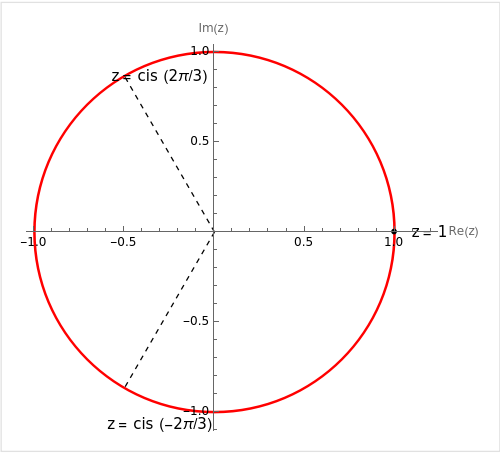
\includegraphics[width = 0.5\textwidth]{rootdemoivre.png}
    \caption{Solutions for $z^3=1$}
\end{figure}
The solutions are shown to lie on the unit circle at intervals of \( \frac{2\pi}{3} \) around the circle.
We find that the number of roots, of course, follows that the number of roots equal to the order of expression.

To generalize, we can see that there are exactly $m$ distinct $mth$ roots of unity, denoted
by
 \begin{equation}
    \boxed{1^{1/m}=e^{i2k\pi/m}=\cos\frac{2k\pi}m+i\sin\frac{2k\pi}m\quad(k=0,1,2, \ldots, m-1).}
 \end{equation}

\begin{theorem}[Solution of \( z^n = a \)] 

    For \( n \in \mathbb{N} \) and \( a \in \mathbb{C} \), the solutions of the equation \( z^n = a \) are called the \textit{n}th roots of \( a \).
\begin{itemize}[leftmargin=*]
    \item The solutions of \( z^n = a \) lie on a circle with center the origin and radius \( |a|^{1/n} \).
    \item There are \( n \) solutions and they are equally spaced around the circle at intervals of \( \frac{2\pi}{n} \). This observation can be used to find all solutions if one is known.
\end{itemize}
\end{theorem}   
More generally, consider any natural number \( n \geq 2 \). Using De Moivre's theorem, we can show that the \( n \)th roots of unity are
\[
1, \, \text{cis}\left(\frac{2\pi}{n}\right), \, \text{cis}\left(\frac{4\pi}{n}\right), \, \ldots, \, \text{cis}\left(\frac{2(n-1)\pi}{n}\right)
\]
So the \( n \)th roots of unity form a geometric sequence with common ratio \( \omega = \text{cis}\left(\frac{2\pi}{n}\right) \).
We can list the terms of this sequence as \( 1, \omega, \omega^2, \ldots, \omega^{n-1} \). The sum of the terms is
\[
1 + \omega + \omega^2 + \ldots + \omega^{n-1} = \frac{\omega^n - 1}{\omega - 1}
\]
since \( \omega^n = 1 \).
\begin{proof}
    The \( n \)th roots of unity are solutions to the equation \( z^n = 1 \). By expressing 1 in polar form as \( 1 \text{cis} 0 \), and applying De Moivre's theorem, \( (r \text{cis} \theta)^n = r^n \text{cis} (n\theta) \), we find that for \( z^n = 1 \), we must have \( z = \text{cis} \left(\frac{2k\pi}{n}\right) \), where \( k \) is an integer from \( 0 \) to \( n-1 \).

These solutions can be written as a sequence where each term after the first is obtained by multiplying the previous term by \( \text{cis} \left(\frac{2\pi}{n}\right) \), making it a geometric sequence with a common ratio of \( \omega = \text{cis} \left(\frac{2\pi}{n}\right) \).

The sum of a geometric sequence with \( n \) terms and a common ratio \( r \neq 1 \) is given by \( S_n = a_1 \frac{1-r^n}{1-r} \). For our sequence, \( a_1 = 1 \) and \( r = \omega \), so the sum is \( S_n = \frac{1-\omega^n}{1-\omega} \). Since \( \omega^n = \text{cis} (2\pi) = 1 \), the numerator becomes \( 1-1 = 0 \), hence the sum \( S_n \) is zero.
\end{proof}

To obtain the \( m \)th roots of an \textit{arbitrary} (nonzero) complex number \( z = re^{i\theta} \), we generalize the idea and, reasoning similarly, conclude that the \( m \) distinct \( m \)th roots of \( z \) are given by
\begin{equation}\label{mthroot}
    \boxed{z^{1/m} = \sqrt[m]{|z|}e^{i(\theta+2k\pi)/m} \quad (k = 0, 1, 2, \ldots, m - 1)}
\end{equation}

Equivalently, we can form these roots by taking any single one such as given in (3) and multiplying by the \( m \)th roots of unity.

\begin{example}
    Find all the cube roots of \( \sqrt{2} + i\sqrt{2} \).
\end{example}
\textbf{Solution:}
The polar form for \( \sqrt{2} + i\sqrt{2} \) is
\[
\sqrt{2} + i\sqrt{2} = 2e^{i\pi/4}.
\]
Putting \( |z| = 2 \), \( \theta = \pi/4 \), and \( m = 3 \) into Eq. \ref{mthroot}, we obtain
\[
(\sqrt{2} + i\sqrt{2})^{1/3} = \sqrt[3]{2}e^{i(\pi/12+2k\pi/3)} \quad (k = 0, 1, 2).
\]
Therefore, the three cube roots of \( \sqrt{2} + i\sqrt{2} \) are \( \sqrt[3]{2}(cos \pi/12 + i \sin \pi/12) \), \( \sqrt[3]{2}(cos 3\pi/4 + i \sin 3\pi/4) \), and \( \sqrt[3]{2}(cos 17\pi/12 + i \sin 17\pi/12) \).
\subsection{Exercises}

\begin{exercise}
    Let \( P(z) = 2z^3 + 9z^2 + 14z + 5 \).

\begin{itemize}
    \item[\textbf{a.}] Use the factor theorem to show that \( z + 2 - i \) is a linear factor of \( P(z) \).
    \item[\textbf{b.}] Write down another complex linear factor of \( P(z) \).
    \item[\textbf{c.}] Hence find all the linear factors of \( P(z) \) over \( \mathbb{C} \).
\end{itemize}
\end{exercise}
\textbf{Solution}

\textbf{a.} By the factor theorem, if \( z + 2 - i \) is a factor of \( P(z) \), then \( P(-2 + i) = 0 \). Calculating this we get:
\begin{align*}
P(-2 + i) &= 2(-2 + i)^3 + 9(-2 + i)^2 + 14(-2 + i) + 5 \\
&= 2(-8 - 12i + 6i^2) + 9(4 - 8i + 2i^2) + 14(-2 + i) + 5 \\
&= 2(-8 - 12i - 6) + 9(4 - 8i - 2) + (-28 + 14i) + 5 \\
&= -28 - 24i - 12 + 36 - 72i - 18 - 28 + 14i + 5 \\
&= 0.
\end{align*}
Thus, \( z + 2 - i \) is a linear factor of \( P(z) \).

\textbf{b.} By the conjugate root theorem, if \( z + 2 - i \) is a root, then its conjugate \( z + 2 + i \) is also a root.

\textbf{c.} Having found two complex roots, we can divide \( P(z) \) by the product of the corresponding factors to find the remaining factor. Let's perform the division (this is a mock example; the actual division should be computed):

% Example of polynomial division (mock)
\begin{align*}
P(z) &= (z + 2 - i)(z + 2 + i)(z - \alpha) \\
\end{align*}

After performing the division, we find that the remaining factor is \( z - \frac{1}{2} \). Thus, the linear factors of \( P(z) \) are:

\[
P(z) = (z + 2 - i)(z + 2 + i)\left(z - \frac{1}{2}\right)
\]

\begin{exercise}
    For a cubic polynomial \(P(x)\) with real coefficients, it is given that \(P(2 + i) = 0\), \(P(1) = 0\) and \(P(0) = 10\). Express \(P(x)\) in the form \(P(x) = ax^3 + bx^2 + cx + d\) and solve the equation \(P(x) = 0\).
\end{exercise}
\textbf{solution:}

Given that \(P(x)\) is a cubic polynomial with real coefficients and \(P(2 + i) = 0\), we know that its conjugate \(P(2 - i) = 0\) as well, due to the complex conjugate root theorem. Moreover, since \(P(1) = 0\), we can write \(P(x)\) as:

\[ P(x) = a(x - (2 + i))(x - (2 - i))(x - 1) \]

Expanding this and simplifying, we get:

\[ P(x) = a((x - 2)^2 + 1)(x - 1) \]

Since \(P(0) = 10\), we can find \(a\) by substituting \(x = 0\):

\[ 10 = a((0 - 2)^2 + 1)(0 - 1) \]
\[ 10 = a(4 + 1)(-1) \]
\[ 10 = -5a \]
\[ a = -2 \]

Thus, the polynomial is:

\[ P(x) = -2((x - 2)^2 + 1)(x - 1) \]
\[ P(x) = -2(x^2 - 4x + 4 + 1)(x - 1) \]
\[ P(x) = -2(x^2 - 4x + 5)(x - 1) \]
\[ P(x) = -2(x^3 - x^2 - 4x^2 + 4x + 5x - 5) \]
\[ P(x) = -2x^3 + 10x^2 - 18x + 10 \]

To solve for \(P(x) = 0\), we now have the equation:

\[ -2x^3 + 10x^2 - 18x + 10 = 0 \]

Since $P(2+i) = 0$, by conjugate root theorem, $p(2-i) = 0$, and we also have $p(1) = 0$.
The order of this expression is 3, by the fundamental algebra theorem, we have found all solutions.

\begin{exercise}
    If \( z = 1 + i \) is a zero of the polynomial \( z^3 + az^2 + bz + 10 - 6i \), find the constants \( a \) and \( b \), given that they are real.
\end{exercise}
\textbf{solution:}

Since \( z = 1 + i \) is a zero, by the Complex Conjugate Root Theorem, \( z = 1 - i \) is also a zero. Substituting \( z = 1 + i \) into the polynomial gives:

\begin{align*}
(1 + i)^3 + a(1 + i)^2 + b(1 + i) + 10 - 6i &= 0 \\
(1 + 3i - 3 - i) + a(1 + 2i - 1) + b + 10 - 6i &= 0 \\
(-2 + 2i) + a(2i) + b + 10 - 6i &= 0 \\
(-2 + (2a - 6)i) + b + 10 &= 0
\end{align*}

For the polynomial to be zero, both the real and imaginary parts must be zero. Therefore, we have two equations:

\begin{align*}
-2 + b + 10 &= 0 \quad \text{(Real part)} \\
2a - 6 &= 0 \quad \text{(Imaginary part)}
\end{align*}

Solving these equations gives us \( a \) and \( b \):

\begin{align*}
b &= -8 \\
a &= 3
\end{align*}

Thus, the constants are \( a = 3 \) and \( b = -8 \).

\begin{exercise}
    Let \( n \) be a positive integer. Prove that \[ \text{arg}(z^n) = n \text{Arg}(z) + 2k\pi, \quad k = 0, \pm1, \pm2, \ldots, \]
    \textbf{for} \( z \neq 0 \)
\end{exercise}
\begin{proof}
    Let's take \( z \in \mathbb{C} \). We can write \( z \) in its polar form as
\[ z = |z|(\cos \theta + i \sin \theta) \]

By definition of arg\( z \) and Arg\( z \) we have: \( \text{arg}(z) = \theta + 2k\pi, k \in \mathbb{Z}, \theta \in [-\pi, \pi] \) and \( \text{Arg}(z) = \text{arg}_{-}(z) = \theta, \theta \in [-\pi, \pi] \).

Now if we take the polar form of \( z^n \), where \( n \in \mathbb{N}, n \neq 0 \), we have
\[ z^n = |z|^n(\cos(n\theta) + i \sin(n\theta)) \]

\[ \Rightarrow \text{arg}(z^n) = n\theta + 2k\pi \]
\[ = n\text{Arg}(z) + 2k\pi, \quad k \in \mathbb{Z} \]

This concludes the proof.
\end{proof}

\begin{exercise}
    Find all the values of the following.
    \begin{enumerate}
        \item[(a)] \( (-16)^{1/4} \)
        \item[(b)] \( 1^{1/5} \)
        \item[(c)] \( i^{1/4} \)
        \item[(d)] \( (1 - \sqrt{3}i)^{1/3} \)
        \item[(e)] \( (i - 1)^{1/2} \)
        \item[(f)] \( \left(\frac{2i}{1+i}\right)^{1/6} \)
    \end{enumerate}
\end{exercise}



\begin{exercise}
    Find all four roots of the equation \( z^4 + 1 = 0 \) and use them to deduce the factorization \( z^4 + 1 = (z^2 - \sqrt{2}z + 1)(z^2 + \sqrt{2}z + 1) \).
\end{exercise}
\textbf{Solution:}

First, we solve the equation:
\begin{align*}
z^4 + 1 &= 0 \\
z^4 &= -1 \\
z &= \sqrt[4]{-1}
\end{align*}

Since \( -1 = \cos \pi + i \sin \pi \), we can find the roots using De Moivre's theorem:
\[ z = \sqrt[4]{\cos \pi + i \sin \pi} = \sqrt[4]{1}(\cos (\pi + 2k\pi)/4 + i \sin (\pi + 2k\pi)/4), \quad k = 0,1,2,3 \]

Thus, the roots are:
\begin{align*}
z_0 &= \cos \frac{\pi}{4} + i \sin \frac{\pi}{4} = \frac{1}{\sqrt{2}} + i \frac{1}{\sqrt{2}} \\
z_1 &= \cos \frac{3\pi}{4} + i \sin \frac{3\pi}{4} = -\frac{1}{\sqrt{2}} + i \frac{1}{\sqrt{2}} \\
z_2 &= \cos \frac{5\pi}{4} + i \sin \frac{5\pi}{4} = -\frac{1}{\sqrt{2}} - i \frac{1}{\sqrt{2}} \\
z_3 &= \cos \frac{7\pi}{4} + i \sin \frac{7\pi}{4} = \frac{1}{\sqrt{2}} - i \frac{1}{\sqrt{2}}
\end{align*}

To show the factorization, we pair the roots:
\begin{align*}
z^4 + 1 &= (z - z_0)(z - z_1)(z - z_2)(z - z_3) \\
&= \left(z - \frac{1}{\sqrt{2}} - i \frac{1}{\sqrt{2}}\right)\left(z + \frac{1}{\sqrt{2}} - i \frac{1}{\sqrt{2}}\right) \\
&\quad \times \left(z + \frac{1}{\sqrt{2}} + i \frac{1}{\sqrt{2}}\right)\left(z - \frac{1}{\sqrt{2}} + i \frac{1}{\sqrt{2}}\right) \\
&= \left(z^2 - \sqrt{2}z + 1\right)\left(z^2 + \sqrt{2}z + 1\right)
\end{align*}

And we have shown the factorization.

\begin{exercise}
    Let \( \alpha \) and \( \beta \) be the mth and nth roots of unity, respectively. We want to show that the product \( \alpha\beta \) is a kth root of unity for some integer \( k \).
\end{exercise}
\textbf{Solution:}

Let's consider \( \alpha \) as the m-th root of unity and \( \beta \) the n-th root of unity. Then we have
\[ \alpha^m = 1 \]
\[ \beta^n = 1 \]

Let's show that \( \alpha\beta \) is a root of unity. If \( \alpha\beta \) is a root of unity then there exists some \( l \in \mathbb{N} \) such that \( (\alpha\beta)^l = 1 \).

For \( l = mn \) (since \( m \) and \( n \) are relatively prime), we have
\[ (\alpha\beta)^l = (\alpha\beta)^{mn} \]
\[ = \alpha^{mn}\beta^{mn} \]
\[ = (\alpha^m)^n(\beta^n)^m \]
\[ = 1^n1^m \]
\[ = 1 \]

Thus, \( \alpha\beta \) is indeed a root of unity, specifically an \( mn \)-th root of unity.

\begin{exercise}
    Let \( m \) and \( n \) be positive integers that have no common factor. Prove that the set of numbers \( (z^{1/n})^m \) is the same as the set of numbers \( (z^m)^{1/n} \). We denote this common set of numbers by \( z^{m/n} \). Show that
\[ z^{m/n} = \sqrt[n]{|z|^m} \left[ \cos \left( \frac{m}{n} (\theta + 2k\pi) \right) + i \sin \left( \frac{m}{n} (\theta + 2k\pi) \right) \right] \]
for \( k = 0, 1, \ldots, n - 1 \).
\end{exercise}
\begin{proof}
    Let's take \( m, n \in \mathbb{N} \) so that they are relatively prime and \( z \in \mathbb{C} \) so that \( \text{Arg}(z) = \theta \). We have:
\begin{align*}
(z^{1/n})^m &= (\sqrt[n]{z})^m = \left( \sqrt[n]{|z|e^{i\theta}} \right)^m \\
&= \left( \sqrt[n]{|z|}e^{i\theta/n} \right)^m \\
&= |z|^{m/n} e^{im\theta/n}
\end{align*}

Now as \( m \) and \( n \) are relatively prime we have
\[ \frac{2k\pi}{n} \frac{m}{n} \quad k = 0, \ldots, n - 1 \]
from where
\begin{align*}
|z|^{m/n} e^{im(\theta + 2k\pi)/n} &= |z|^{m/n} e^{im\theta/n + im2k\pi/n} \\
&= (|z|^m)^{1/n} (e^{im\theta})^{1/n} \\
&= ((|z|^m e^{im\theta})^{1/n} \\
&= (z^m)^{1/n}
\end{align*}

To show the expression we take the previous result and expand it:
\begin{align*}
z^{m/n} &= |z|^{m/n} e^{im\theta/n} \\
&= \sqrt[n]{|z|^m} \left[ \cos \left( \frac{m\theta}{n} + \frac{2km\pi}{n} \right) + i \sin \left( \frac{m\theta}{n} + \frac{2km\pi}{n} \right) \right] \\
&= \sqrt[n]{|z|^m} \left[ \cos \left( \frac{m}{n} (\theta + 2k\pi) \right) + i \sin \left( \frac{m}{n} (\theta + 2k\pi) \right) \right]
\end{align*}
\end{proof}


\begin{exercise}
    Use the conclusion in last problem to evaluate $(i-i)^\frac{3}{2}$.
\end{exercise}
\textbf{Solution:}
It has been shown that
\begin{equation}
    \boxed{ z^{m/n} = \sqrt[n]{|z|^m}\left[\cos\left(\frac{m}{n}(\theta + 2k\pi)\right) + i\sin\left(\frac{m}{n}(\theta + 2k\pi)\right)\right]}
\end{equation}
We have:
\[ z = (1 - i)^{3/2} \Rightarrow m = 3, n = 2 \]
\[ |z| = \sqrt{1^2 + (-1)^2} = \sqrt{2} \]
\[ \theta = \text{Arg} z = 2\pi - \cot^{-1}\left(\frac{-1}{1}\right) = \frac{7\pi}{4} \]

When we put everything in the formula we get
\[ z = \sqrt[2]{\sqrt{2}^3}\left[\cos\left(\frac{3}{2}\left(\frac{7\pi}{4} + 2k\pi\right)\right) + i\sin\left(\frac{3}{2}\left(\frac{7\pi}{4} + 2k\pi\right)\right)\right], k = 0, 1 \]
\[ z = \sqrt[2]{2^{3/2}}\left[\cos\left(\frac{21\pi}{8} + \frac{3k\pi}{2}\right) + i\sin\left(\frac{21\pi}{8} + \frac{3k\pi}{2}\right)\right], k = 0, 1 \]
\[ z_0 = 2^{3/4}\left[\cos\left(\frac{21\pi}{8}\right) + i\sin\left(\frac{21\pi}{8}\right)\right] \]
\[ z_1 = 2^{3/4}\left[\cos\left(\frac{21\pi}{8} + \frac{3\pi}{2}\right) + i\sin\left(\frac{21\pi}{8} + \frac{3\pi}{2}\right)\right] \]
%------------------------------------------------
\part{Further Discrete Mathematics}


\chapterimage{orange2.jpg}
\chapterspaceabove{6.75cm} 
\chapterspacebelow{7.25cm} 
\chapter{Boolean Algebra}

%------------------------------------------------
\chapterimage{orange2.jpg}
\chapterspaceabove{6.75cm} 
\chapterspacebelow{7.25cm} 
\chapter{Preliminary Number Theory}
%------------------------------------------------
\chapterimage{orange2.jpg}
\chapterspaceabove{6.75cm} 
\chapterspacebelow{7.25cm} 
\chapter{Search and Sorting}
%------------------------------------------------
\chapterimage{orange2.jpg}
\chapterspaceabove{6.75cm} 
\chapterspacebelow{7.25cm} 
\chapter{Graph Theory}

%------------------------------------------------
\part{Single-variable Calculus}
%------------------------------------------------
\part{Multi-variable and Vector Calculus}
%------------------------------------------------

\part{Linear Algebra}
%------------------------------------------------
\part{Probability and Combinatorics}

\chapterimage{orange2.jpg}
\chapterspaceabove{6.75cm} 
\chapterspacebelow{7.25cm} 
\chapter{Counting Method and Basic Combinatorics}


\chapterimage{orange2.jpg}
\chapterspaceabove{6.75cm} 
\chapterspacebelow{7.25cm} 
\chapter{Probability Theorems}


\chapterimage{orange2.jpg}
\chapterspaceabove{6.75cm} 
\chapterspacebelow{7.25cm} 
\chapter{Discrete Distribution}


\chapterimage{orange2.jpg}
\chapterspaceabove{6.75cm} 
\chapterspacebelow{7.25cm} 
\chapter{Continuous Distribution}


\chapterimage{orange2.jpg}
\chapterspaceabove{6.75cm} 
\chapterspacebelow{7.25cm} 
\chapter{Joint Cumulative Distribution}
%------------------------------------------------
\part{Statistics}


%----------------------------------------------------------------------------------------

\stopcontents[part] % Manually stop the 'part' table of contents here so the previous Part page table of contents doesn't list the following chapters



\end{document}
